% ============================================================================
%  Capítulo 5 - Aspectos prácticos de implementación
% ============================================================================
\chapter{Aspectos prácticos de implementación}
\label{cap:implementacion}
En este capítulo se tratan algunos aspectos prácticos de implementación que se deben
considerar a la hora de utilizar el ADRC ya en la puesta en marcha, para tener el mejor
funcionamiento posible: el manejo de la saturación, el acondicionamiento de la referencia,
el manejo del ruido y la discretización, para poder usarlo en equipos digitales. Al
finalizar el capítulo se resume toda una metodología de implementación para llegar a
utilizar el ADRC desde la teoría hasta la puesta en marcha.

%--------------------------------------------------------------------
\section{Manejo de la saturación}
\label{sec:impl_saturacion}

%--------------------------------------------------------------------
\subsection{Saturación ADRC basado en observador}
\label{subsec:sat_adrc}

El soplador solo puede entregar entre $0$ y $100~\%$, así que la orden que
llega a la planta no es $u(t)$, sino su versión limitada
\cite[sec.~9.1.1]{herbst2024adrc},
\begin{equation}
u_{\mathrm{sat}}(t) = \operatorname{sat}\bigl(u(t)\bigr) =
\begin{cases}
0~\%, & u(t) < 0~\%, \\
u(t), & 0~\% \le u(t) \le 100~\%, \\
100~\%, & u(t) > 100~\%,
\end{cases}
\qquad u(t) = \frac{u_0(t)}{b_0}.
\label{eq:saturacion}
\end{equation}
Si el observador siguiera recibiendo $u_0(t)$, estimaría el efecto de una orden
que la planta no recibió: la diferencia entre $u$ y $u_{\mathrm{sat}}$
aparecería como perturbación en $\hat{\xi}$ y la ley de control la seguiría
acumulando, que es el \emph{windup} del ADRC. Para evitarlo, al observador se le
realimenta la orden aplicada, multiplicada por $b_0$ para que vuelva a las
unidades de $u_0$ (Figura~\ref{fig:adrc_saturacion}; en la Figura~\ref{fig:simulink_eso} se
muestra el mismo esquema con bloques de Simulink):
\begin{equation}
\dot{\widehat{\mathbf{X}}}(t) =
\bigl(\mathbf{A} - \mathbf{L}\,\mathbf{C}\bigr)\,\widehat{\mathbf{X}}(t)
+ \mathbf{B}\,b_0\,u_{\mathrm{sat}}(t) + \mathbf{L}\,e_y(t).
\label{eq:observador_saturacion}
\end{equation}
Así, el ADRC con observador de estado extendido trae su propio
\emph{anti-windup}: según Herbst y Madoński, realimentar la señal limitada en
lugar de $u$ es la única medida necesaria, y no añade parámetros que sintonizar
\cite[sec.~9.1.1]{herbst2024adrc}, lo que resulta en una forma muy fácil y eficiente de
manejar la saturación.


\begin{figure}[H]
  \centering
  \resizebox{\textwidth}{!}{%
  \begin{tikzpicture}[every path/.style={thick}]

    % --- Nodos principales ---
    \node[sum] (s1) at (1.4,0) {};

    \node[block, minimum width=4.4cm, minimum height=1.9cm] (obs) at (5.9,-0.4)
      {$\mathbf{A}_o\widehat{\mathbf{X}}(t) + \mathbf{B}_o \mathbf{u}_t(t)$ \\[10pt] $\mathbf{C}_o\widehat{\mathbf{X}}(t) + \mathbf{D}_o \mathbf{u}_t(t)$};
    \node[above=1pt of obs] {Observador};

    \node[block, minimum size=9mm] (K) at (9.6,0) {$-\mathbf{K}$};
    \coordinate (u0) at (10.7,0);
    \node[block, minimum size=9mm] (ib) at (11.7,0) {$1/b_0$};

    % saturacion (icono clasico de Simulink)
    \node[block, minimum size=11mm] (sat) at (13.9,0) {};
    \draw[thin, gray] ($(sat.center)+(-0.38,0)$) -- ($(sat.center)+(0.38,0)$);
    \draw[thin, gray] ($(sat.center)+(0,-0.38)$) -- ($(sat.center)+(0,0.38)$);
    \draw[line width=1.1pt] ($(sat.center)+(-0.38,-0.22)$) -- ($(sat.center)+(-0.18,-0.22)$)
                         -- ($(sat.center)+(0.18,0.22)$) -- ($(sat.center)+(0.38,0.22)$);
    \node[above=1pt of sat, font=\small] {0--100~\%};

    \coordinate (us) at (15.3,0);
    \node[sum] (s2) at (16.7,0) {};

    \node[block, minimum width=3.6cm, minimum height=1.9cm] (plant) at (20.0,0)
      {$\mathbf{A}_g \mathbf{x}_g(t) + \mathbf{B}_g \bar{u}(t)$ \\[10pt] $\mathbf{C}_g \mathbf{x}_g(t) + \mathbf{D}_g \bar{u}(t)$};

    \coordinate (yb) at (22.4,0);

    % ganancia b0 en la realimentacion hacia el observador
    \node[block, minimum size=9mm] (gb) at (9.6,-1.9) {$b_0$};

    % --- Recuadro ADRC ---
    \draw[red, dashed, thick] (3.0,1.6) rectangle (12.4,-2.6);
    \node[below left] at (12.4,1.6) {ADRC};

    % --- Señales ---
    \draw[->] (0,0) node[above right] {$r(t)$} -- (s1.west);
    \node[sgn] at ($(s1.west)+(-0.15,0.25)$) {$-$};

    \draw[->] (s1.east) -- node[above, pos=0.45] {$e_y(t)$} (obs.west |- s1);
    \draw[->] (obs.east |- K) -- node[above] {$\widehat{\mathbf{X}}(t)$} (K.west);

    \draw (K.east) -- (u0) node[above] {$u_0(t)$};
    \draw[->] (u0) -- (ib.west);
    \draw[->] (ib.east) -- node[above, pos=0.6] {$u(t)$} (sat.west);
    \draw (sat.east) -- (us) node[above] {$u_{\mathrm{sat}}(t)$};
    \fill (us) circle (1.5pt);
    \draw[->] (us) -- (s2.west);
    \node[sgn] at ($(s2.west)+(-0.2,0.25)$) {$+$};

    % u_sat -> b0 -> observador
    \draw[->] (us) -- (us |- 0,-1.9) -- (gb.east);
    \draw[->] (gb.west) -- (3.35,-1.9) node[below right] {$b_0\,u_{\mathrm{sat}}(t)$}
              -- (3.35,-0.85) -- (obs.west |- 0,-0.85);

    \draw[->] (s2 |- 0,1.6) node[above] {$\varepsilon(t)$} -- (s2.north);
    \node[sgn] at ($(s2.north)+(-0.25,0.2)$) {$+$};

    \draw[->] (s2.east) -- node[above] {$\bar{u}(t)$} (plant.west);

    \draw (plant.east) -- (yb);
    \draw[->] (yb) -- (23.5,0) node[above left] {$y(t)$};
    \fill (yb) circle (1.5pt);

    \draw[->] (yb) -- (22.4,-3.2) -- (1.4,-3.2) -- (s1.south);
    \node[sgn] at ($(s1.south)+(-0.25,-0.15)$) {$+$};
    \node[right] at ($(s1.south)+(0,-0.45)$) {$y(t)$};

  \end{tikzpicture}%
  }
  \caption[ADRC con saturación del actuador]{ADRC con saturación del actuador.
    La orden $u = u_0/b_0$ se limita entre $0$ y $100~\%$, y al observador se le
    realimenta la orden aplicada, $b_0\,u_{\mathrm{sat}}$, que está en las
    unidades de $u_0$.}
  \label{fig:adrc_saturacion}
\end{figure}

\begin{figure}[H]
  \centering
  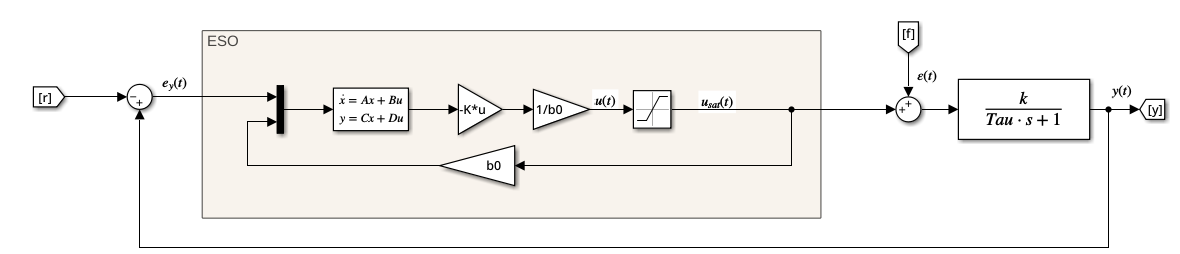
\includegraphics[width=\textwidth]{simulink_eso_saturacion.png}
  \caption[Implementación en Simulink del ADRC con saturación]{Implementación
    en Simulink del ADRC con observador, saturación del actuador y realimentación
    de la orden aplicada al observador.}
  \label{fig:simulink_eso}
\end{figure}

La Figura~\ref{fig:adrc_lazo_cerrado_saturacion} repite la simulación de la
Figura~\ref{fig:adrc_lazo_cerrado} con el soplador limitado y el observador
realimentado con $b_0\,u_{\mathrm{sat}}$. Al arrancar, el soplador se queda en
$100~\%$ unos $5{,}4$~min y el oxígeno sube más despacio (alcanza el $63~\%$ del
primer escalón en $5{,}9$~min, frente a $1{,}6$~min sin saturación), pero sin
sobreimpulso ni \emph{windup}: en cuanto la salida se acerca a la consigna, $u$
deja el límite y vuelve la dinámica diseñada. En el panel (c) se ve la perturbación exógena
aplicada y la perturbación total estimada: al entrar un cambio de referencia, el observador lo
estima como parte de la perturbación total, por lo que se ve un pico enorme que luego vuelve al
estado estacionario.


En el cambio de la referencia de $2{,}0$ a $2{,}2$~mg/L se ve el mismo comportamiento
que en el caso sin el manejo de saturación: cerca del
punto de operación de $2$~mg/L, el controlador regula y sigue cambios pequeños
de consigna sin llegar a los límites. Esta es la ventaja del esquema: sigue y
rechaza distintos tipos de señales con solo incluirlas en el modelo interno.
Su desventaja es que, con escalones grandes o una sintonía agresiva, puede
saturar el actuador. Para seguir consignas tipo escalón sin saturar, la
referencia se suaviza antes de entrar al controlador, ya sea, como se presenta en este
documento, con una curva de Bézier o con un prefiltro de la señal de consigna, de modo que la salida llegue a la consigna de forma gradual sin que la señal
de control se sature (Sección~\ref{sec:impl_referencia}).


\begin{figure}[H]
  \centering
  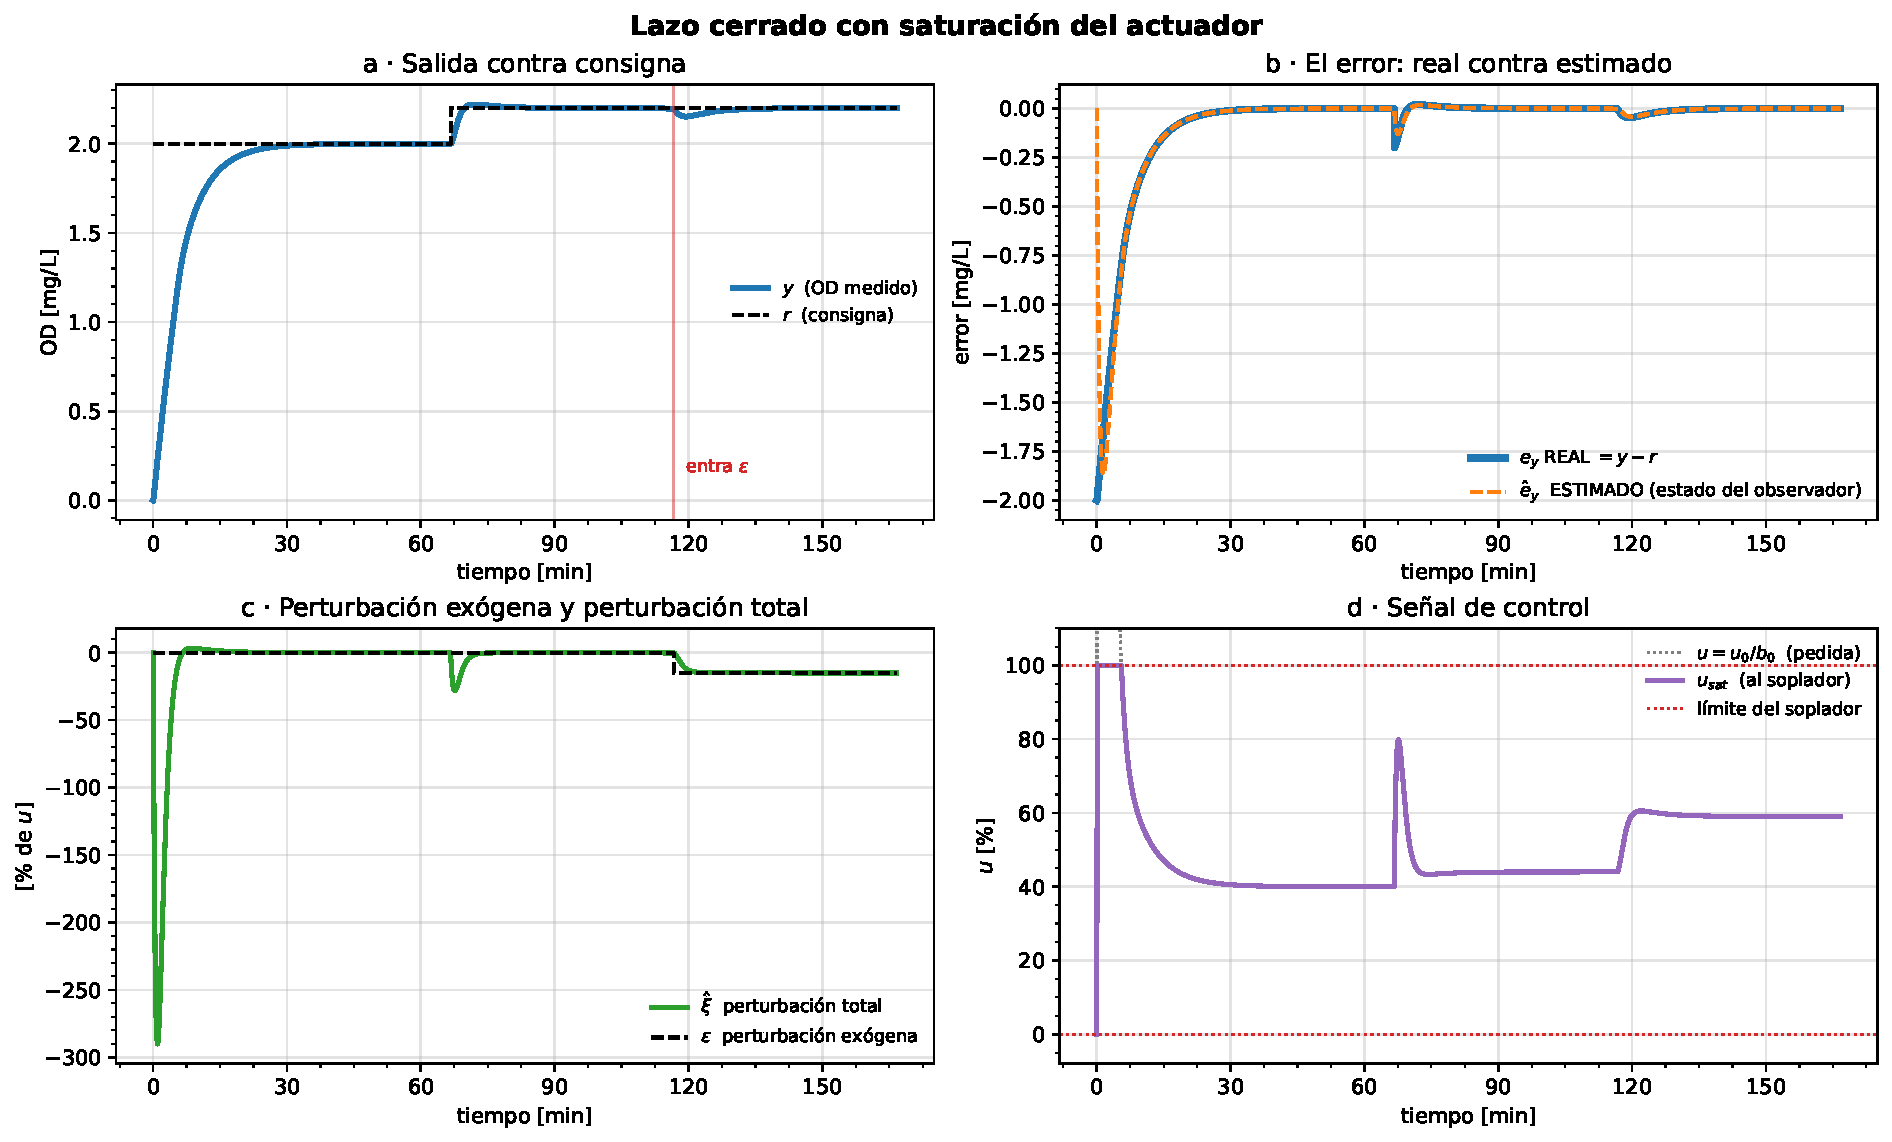
\includegraphics[width=\textwidth]{adrc_lazo_cerrado_saturacion.pdf}
  \caption[Lazo cerrado del ADRC con saturación del actuador]{Lazo cerrado del
    ADRC con la planta y el soplador limitado entre $0$ y $100~\%$.
    (a) Salida contra consigna. (b) Error de seguimiento real y estimado.
    (c) Perturbación exógena y perturbación total, en \% de $u$. (d) Orden
    pedida por el controlador y orden aplicada.}
  \label{fig:adrc_lazo_cerrado_saturacion}
\end{figure}

%--------------------------------------------------------------------
\subsection{Saturación del GPI robusto}
\label{subsec:sat_gpi}
\begin{figure}[H]
  \centering
  \resizebox{\textwidth}{!}{%
  \begin{tikzpicture}[every path/.style={thick}]
    \node[sum] (s1) at (1.2,0) {};
    \node[block, minimum width=2.0cm, minimum height=1.3cm] (pe) at (3.9,0)
      {$\dfrac{P(s)}{E_1(s)}$};
    \node[sum] (s2) at (6.2,0) {};

    % saturacion (icono clasico de Simulink)
    \node[block, minimum size=11mm] (sat) at (8.0,0) {};
    \draw[thin, gray] ($(sat.center)+(-0.38,0)$) -- ($(sat.center)+(0.38,0)$);
    \draw[thin, gray] ($(sat.center)+(0,-0.38)$) -- ($(sat.center)+(0,0.38)$);
    \draw[line width=1.1pt] ($(sat.center)+(-0.38,-0.22)$) -- ($(sat.center)+(-0.18,-0.22)$)
                         -- ($(sat.center)+(0.18,0.22)$) -- ($(sat.center)+(0.38,0.22)$);
    \node[above=1pt of sat, font=\small] {0--100~\%};

    \coordinate (us) at (9.6,0);
    \node[block, minimum width=2.4cm, minimum height=1.3cm] (fb) at (7.9,-1.9)
      {$\dfrac{L(s) - E_1(s)}{E_1(s)}$};
    \node[sum] (s3) at (11.4,0) {};
    \node[block, minimum width=2.4cm, minimum height=1.3cm] (plant) at (13.9,0)
      {$G(s)$};
    \coordinate (yb) at (16.1,0);

    % --- recuadro del controlador ---
    \draw[red, dashed, thick] (2.5,1.85) rectangle (10.1,-2.85);
    \node[below left] at (10.1,1.85) {GPI con \emph{anti-windup}};

    % --- señales ---
    \draw[->] (-0.3,0) node[above right] {$r(t)$} -- (s1.west);
    \node[sgn] at ($(s1.west)+(-0.15,0.25)$) {$+$};
    \draw[->] (s1.east) -- node[above, pos=0.35] {$-e_y(t)$} (pe.west);
    \draw[->] (pe.east) -- (s2.west);
    \node[sgn] at ($(s2.west)+(-0.2,0.25)$) {$+$};
    \draw[->] (s2.east) -- node[above] {$v(t)$} (sat.west);
    \draw (sat.east) -- (us);
    \fill (us) circle (1.5pt);
    \draw[->] (us) -- node[above, pos=0.62] {$u_{\mathrm{sat}}(t)$} (s3.west);
    \node[sgn] at ($(s3.west)+(-0.2,-0.25)$) {$+$};
    \draw[->] (s3 |- 0,1.6) node[above] {$\xi(t)$} -- (s3.north);
    \node[sgn] at ($(s3.north)+(0.25,0.2)$) {$+$};
    \draw[->] (s3.east) -- node[above] {$\bar{u}(t)$} (plant.west);
    \draw[->] (us) -- (us |- fb) -- (fb.east);
    \draw[->] (fb.west) -- (s2 |- fb) -- (s2.south);
    \node[sgn] at ($(s2.south)+(-0.25,-0.2)$) {$-$};
    \draw (plant.east) -- (yb);
    \draw[->] (yb) -- (17.2,0) node[above left] {$y(t)$};
    \fill (yb) circle (1.5pt);
    \draw[->] (yb) -- (16.1,-3.3) -- (1.2,-3.3) -- (s1.south);
    \node[sgn] at ($(s1.south)+(-0.25,-0.15)$) {$-$};
  \end{tikzpicture}%
  }
  \caption[GPI con realimentación de la saturación]{Implementación del GPI con
    realimentación de la saturación \cite[sec.~19.1.3]{levine2011handbook}. A
    $E_1(s)$ llega la señal aplicada $u_{\mathrm{sat}}$, no la pedida $v$.}
  \label{fig:gpi_antiwindup}
\end{figure}

\paragraph{Implementación con realimentación de la saturación.} Se utiliza el esquema de saturación del Handbook; para ello, primero 
es necesario saber que todo
controlador lineal puede escribirse como un cociente de polinomios, con $L(s)$
mónico de grado $n$, el mismo punto de partida que usan
Cortés-Romero y colaboradores para el \emph{anti-windup} de un GPI robusto
\cite{vargas2026microgrids}, 
\begin{equation}
u(s) = C(s)\,\bigl(-e_y(s)\bigr) = \frac{P(s)}{L(s)}\,\bigl(-e_y(s)\bigr),
\qquad L(s) = s^{n} + l_{n-1}s^{n-1} + \cdots + l_0 .
\end{equation}
y se puede reescribir realimentando la señal saturada, con un polinomio mónico y estable
$E_1(s)$ del mismo grado $n$ (Figura~\ref{fig:gpi_antiwindup}), esquema obtenido de
\cite[sec.~19.1.3]{levine2011handbook}:
\begin{equation}
v(s) = \frac{P(s)}{E_1(s)}\,\bigl(-e_y(s)\bigr) - \frac{L(s) - E_1(s)}{E_1(s)}\,u_{\mathrm{sat}}(s),
\qquad u_{\mathrm{sat}}(t) = \operatorname{sat}\bigl(v(t)\bigr) .
\label{eq:aw_handbook}
\end{equation}
Cuando el actuador no se satura, $v = u_{\mathrm{sat}} = u$, y se recupera el
controlador original:
\begin{align}
u(s) &= \frac{P(s)}{E_1(s)}\,\bigl(-e_y(s)\bigr) - \frac{L(s) - E_1(s)}{E_1(s)}\,u(s) \nonumber\\[4pt]
u(s)\left[1 + \frac{L(s) - E_1(s)}{E_1(s)}\right] &= \frac{P(s)}{E_1(s)}\,\bigl(-e_y(s)\bigr) \nonumber\\[4pt]
u(s)\left[\frac{L(s)}{E_1(s)}\right] &= \frac{P(s)}{E_1(s)}\,\bigl(-e_y(s)\bigr) \nonumber\\[4pt]
u(s) &= \frac{P(s)}{L(s)}\,\bigl(-e_y(s)\bigr) .
\end{align}



\paragraph{Anti-windup escrito con las ganancias del GPI.} Para el GPI
\eqref{eq:gpi_ley}, con la planta de diseño $b_0/s$, la orden se calcula en
unidades de $u_0$ y $b_0$ solo convierte a la salida, $u = u_0/b_0$, como en el
ADRC. En unidades de $u_0$ el controlador es
\begin{equation}
C_0(s) = b_0\,C(s) = \frac{k_1 s + k_0}{s\,(s + k_2)} = \frac{P(s)}{L(s)},
\qquad
P(s) = k_1 s + k_0,
\qquad
L(s) = s^2 + k_2 s \quad (n = 2) ,
\end{equation}
y el polinomio característico del lazo es
\begin{equation}
1 + C(s)\,\frac{b_0}{s}
= 1 + \frac{1}{b_0}\,\frac{k_1 s + k_0}{s\,(s + k_2)}\cdot\frac{b_0}{s} = 0
\quad\Longrightarrow\quad
\Delta(s) = s^3 + k_2 s^2 + k_1 s + k_0 .
\end{equation}
El Handbook menciona que $E_1$ puede ser cualquier polinomio mónico y estable del mismo grado
que el denominador del controlador, $L(s)$, y recomienda que esté construido con los polos más
rápidos del lazo cerrado \cite[ec.~19.3]{levine2011handbook}. Para este primer caso, $E_1$ se eligió de forma práctica a partir de las
ganancias, sin calcular los polos, para facilitar la implementación posterior: se toma como $E_1$
el polinomio $\Delta$ sin su término independiente, dividido por $s$, es decir, un polinomio
mónico de grado $2$ construido solo con las ganancias, sin factorizar,
\begin{equation}
E_1(s) = s^2 + k_2 s + k_1 .
\label{eq:aw_E1_ganancias}
\end{equation}
Con $C = C_0/b_0$, el anti-windup \eqref{eq:aw_handbook} deja $1/b_0$ justo
después del bloque de $P/E_1$, y a la rama de realimentación llega la orden
aplicada $u_{\mathrm{sat}}$:
\begin{align}
v_1(s) &= \frac{k_1 s + k_0}{s^2 + k_2 s + k_1}\,\bigl(-e_y(s)\bigr), \nonumber\\[4pt]
v_2(s) &= \frac{\bigl[s^2 + k_2 s\bigr] - \bigl[s^2 + k_2 s + k_1\bigr]}{s^2 + k_2 s + k_1}\,u_{\mathrm{sat}}(s)
= \frac{-k_1}{s^2 + k_2 s + k_1}\,u_{\mathrm{sat}}(s), \nonumber\\[4pt]
v(s) &= \frac{v_1(s)}{b_0} - v_2(s), \qquad u_{\mathrm{sat}}(t) = \operatorname{sat}\bigl(v(t)\bigr) .
\label{eq:aw_gpi}
\end{align}
Ahora bien, $E_1$ es estable siempre que $k_2, k_1 > 0$, y
la ganancia estática de la realimentación interna es exactamente $-k_1/k_1 = -1$,
así que la acción integral se recupera sin restar números casi iguales. Si el
actuador no se satura, $u_{\mathrm{sat}} = v$ y el lazo vuelve a
$u(s) = \frac{1}{b_0}\bigl(P(s)/L(s)\bigr)\bigl(-e_y(s)\bigr) = C(s)\bigl(-e_y(s)\bigr)$.

\begin{figure}[H]
  \centering
  \resizebox{\textwidth}{!}{%
  \begin{tikzpicture}[every path/.style={thick}]
    \node[sum] (s1) at (1.2,0) {};
    \node[block, minimum width=3.0cm, minimum height=1.3cm] (pe) at (4.7,0)
      {$\dfrac{k_1 s + k_0}{s^2 + k_2 s + k_1}$};
    \node[block, minimum size=9mm] (ib) at (7.8,0) {$1/b_0$};
    \node[sum] (s2) at (9.3,0) {};

    % saturacion (icono clasico de Simulink)
    \node[block, minimum size=11mm] (sat) at (11.0,0) {};
    \draw[thin, gray] ($(sat.center)+(-0.38,0)$) -- ($(sat.center)+(0.38,0)$);
    \draw[thin, gray] ($(sat.center)+(0,-0.38)$) -- ($(sat.center)+(0,0.38)$);
    \draw[line width=1.1pt] ($(sat.center)+(-0.38,-0.22)$) -- ($(sat.center)+(-0.18,-0.22)$)
                         -- ($(sat.center)+(0.18,0.22)$) -- ($(sat.center)+(0.38,0.22)$);
    \node[above=1pt of sat, font=\small] {0--100~\%};

    \coordinate (us) at (12.8,0);
    \node[block, minimum width=2.6cm, minimum height=1.3cm] (fb) at (11.0,-1.9)
      {$\dfrac{-k_1}{s^2 + k_2 s + k_1}$};
    \node[sum] (s3) at (14.2,0) {};
    \node[block, minimum width=2.4cm, minimum height=1.3cm] (plant) at (16.7,0)
      {$\dfrac{k_{dc}}{\tau s + 1}$};
    \node[above=1pt of plant] {$G(s)$};
    \coordinate (yb) at (18.8,0);

    % --- recuadro del controlador ---
    \draw[red, dashed, thick] (2.7,1.7) rectangle (13.1,-2.9);
    \node[below left] at (13.1,1.7) {GPI};

    % --- señales ---
    \draw[->] (-0.3,0) node[above right] {$r(t)$} -- (s1.west);
    \node[sgn] at ($(s1.west)+(-0.15,0.25)$) {$+$};
    \draw[->] (s1.east) -- node[above, pos=0.4] {$-e_y(t)$} (pe.west);
    \draw[->] (pe.east) -- node[above] {$v_1(t)$} (ib.west);
    \draw[->] (ib.east) -- (s2.west);
    \node[sgn] at ($(s2.west)+(-0.2,0.25)$) {$+$};
    \draw[->] (s2.east) -- node[above] {$v(t)$} (sat.west);
    \draw (sat.east) -- node[above] {$u_{\mathrm{sat}}(t)$} (us);
    \fill (us) circle (1.5pt);
    \draw[->] (us) -- (s3.west);
    \node[sgn] at ($(s3.west)+(-0.2,-0.25)$) {$+$};
    \draw[->] (s3 |- 0,1.6) node[above] {$\varepsilon(t)$} -- (s3.north);
    \node[sgn] at ($(s3.north)+(-0.25,0.2)$) {$+$};
    \draw[->] (s3.east) -- node[above] {$\bar{u}(t)$} (plant.west);
    \draw[->] (us) -- (us |- fb) -- (fb.east);
    \draw[->] (fb.west) -- (s2 |- fb) -- node[left, pos=0.5] {$v_2(t)$} (s2.south);
    \node[sgn] at ($(s2.south)+(0.25,-0.2)$) {$-$};
    \draw (plant.east) -- (yb);
    \draw[->] (yb) -- (19.9,0) node[above left] {$y(t)$};
    \fill (yb) circle (1.5pt);
    \draw[->] (yb) -- (18.8,-3.4) -- (1.2,-3.4) -- (s1.south);
    \node[sgn] at ($(s1.south)+(-0.25,-0.15)$) {$-$};
  \end{tikzpicture}%
  }
  \caption[GPI con realimentación de la saturación escrito con sus
    ganancias]{GPI con realimentación de la saturación escrito con sus
    ganancias, según \eqref{eq:aw_gpi}: $v = v_1/b_0 - v_2$, con
    $E_1(s) = s^2 + k_2 s + k_1$ en los dos bloques. $1/b_0$ va después del
    bloque $P/E_1$ ($u = u_0/b_0$) y a la rama de realimentación llega la señal
    aplicada $u_{\mathrm{sat}}$.}
  \label{fig:gpi_antiwindup_ganancias}
\end{figure}

\paragraph{Anti-windup escrito con el polinomio del observador.} Como $E_1$ es de libre
elección, también se puede tomar del polinomio característico factorizado. Con las ganancias en
función de los anchos de banda (Tabla~\ref{tab:gpi_eso}),
\begin{equation}
k_2 = \omega_c + 2\omega_o, \qquad k_1 = \omega_o\,(\omega_o + 2\omega_c), \qquad k_0 = \omega_c\,\omega_o^2,
\end{equation}
el polinomio característico se separa en la parte del controlador y la del observador,
\begin{equation}
\Delta(s) = s^3 + k_2 s^2 + k_1 s + k_0 = (s + \omega_c)\,(s + \omega_o)^2 ,
\end{equation}
y se toma como $E_1$ la parte del observador,
\begin{equation}
E_1(s) = (s + \omega_o)^2 = s^2 + 2\omega_o\,s + \omega_o^2 = s^2 + l_1 s + l_2 .
\end{equation}
Con $P(s) = k_1 s + k_0$ y $L(s) = s^2 + k_2 s$, el anti-windup \eqref{eq:aw_handbook} queda
\begin{align}
v_1(s) &= \frac{\omega_o\bigl[(\omega_o + 2\omega_c)\,s + \omega_c\,\omega_o\bigr]}{(s + \omega_o)^2}\,\bigl(-e_y(s)\bigr), \nonumber\\[4pt]
v_2(s) &= \frac{\bigl[s^2 + (\omega_c + 2\omega_o)\,s\bigr] - \bigl[s^2 + 2\omega_o\,s + \omega_o^2\bigr]}{(s + \omega_o)^2}\,u_{\mathrm{sat}}(s)
= \frac{\omega_c\,s - \omega_o^2}{(s + \omega_o)^2}\,u_{\mathrm{sat}}(s), \nonumber\\[4pt]
v(s) &= \frac{v_1(s)}{b_0} - v_2(s), \qquad u_{\mathrm{sat}}(t) = \operatorname{sat}\bigl(v(t)\bigr)
\label{eq:aw_gpi_wo}
\end{align}
(Figura~\ref{fig:gpi_antiwindup_wo}). Este $E_1$ es estable siempre, con el polo
doble en $-\omega_o$, y la ganancia estática de la realimentación interna también
es $-\omega_o^2/\omega_o^2 = -1$. Con él, el GPI con anti-windup es exactamente el
ADRC con observador realimentado con $b_0\,u_{\mathrm{sat}}$
(Sección~\ref{subsec:sat_adrc}), y en el arranque de la
Figura~\ref{fig:sat_arranque} las dos respuestas coinciden exactamente.

Si en cambio se usa el $E_1$ escrito con las ganancias \eqref{eq:aw_E1_ganancias},
la diferencia solo aparece cuando el sistema se satura: la saturación se maneja con
una dinámica un poco distinta. Cualquier $E_1$ es válido siempre que sea estable y
del mismo orden que el denominador del controlador; la versión exacta, la que
coincide con el ADRC, es la escrita con las ganancias del observador. Además, la
Figura~\ref{fig:sat_arranque} muestra el GPI sin anti-windup: al saturarse, la
dinámica se afecta por completo y aparecen sobrepicos enormes. 


\begin{figure}[H]
  \centering
  \resizebox{\textwidth}{!}{%
  \begin{tikzpicture}[every path/.style={thick}]
    \node[sum] (s1) at (1.0,0) {};
    \node[block, minimum width=3.6cm, minimum height=1.3cm] (pe) at (5.0,0)
      {$\dfrac{\omega_o\bigl[(\omega_o + 2\omega_c)\,s + \omega_c\omega_o\bigr]}{(s + \omega_o)^2}$};
    \node[above=1pt of pe] {$H_1(s)$};
    \node[block, minimum size=9mm] (ib) at (8.9,0) {$1/b_0$};
    \node[sum] (s2) at (10.4,0) {};

    % saturacion (icono clasico de Simulink)
    \node[block, minimum size=11mm] (sat) at (12.1,0) {};
    \draw[thin, gray] ($(sat.center)+(-0.38,0)$) -- ($(sat.center)+(0.38,0)$);
    \draw[thin, gray] ($(sat.center)+(0,-0.38)$) -- ($(sat.center)+(0,0.38)$);
    \draw[line width=1.1pt] ($(sat.center)+(-0.38,-0.22)$) -- ($(sat.center)+(-0.18,-0.22)$)
                         -- ($(sat.center)+(0.18,0.22)$) -- ($(sat.center)+(0.38,0.22)$);
    \node[above=1pt of sat, font=\small] {0--100~\%};

    \coordinate (us) at (14.0,0);
    \node[block, minimum width=2.6cm, minimum height=1.3cm] (fb) at (12.1,-1.9)
      {$\dfrac{\omega_c\,s - \omega_o^2}{(s + \omega_o)^2}$};
    \node[below=1pt of fb] {$H_2(s)$};
    \node[sum] (s3) at (15.5,0) {};
    \node[block, minimum width=2.4cm, minimum height=1.3cm] (plant) at (18.0,0)
      {$\dfrac{k_{dc}}{\tau s + 1}$};
    \node[above=1pt of plant] {$G(s)$};
    \coordinate (yb) at (20.1,0);

    % --- recuadro del controlador ---
    \draw[red, dashed, thick] (2.2,1.75) rectangle (14.4,-3.2);
    \node[below left] at (14.4,1.75) {GPI};

    % --- señales ---
    \draw[->] (-0.5,0) node[above right] {$r(t)$} -- (s1.west);
    \node[sgn] at ($(s1.west)+(-0.15,0.25)$) {$+$};
    \draw[->] (s1.east) -- node[above, pos=0.35] {$-e_y(t)$} (pe.west);
    \draw[->] (pe.east) -- node[above] {$v_1(t)$} (ib.west);
    \draw[->] (ib.east) -- (s2.west);
    \node[sgn] at ($(s2.west)+(-0.2,0.25)$) {$+$};
    \draw[->] (s2.east) -- node[above] {$v(t)$} (sat.west);
    \draw (sat.east) -- node[above] {$u_{\mathrm{sat}}(t)$} (us);
    \fill (us) circle (1.5pt);
    \draw[->] (us) -- (s3.west);
    \node[sgn] at ($(s3.west)+(-0.2,-0.25)$) {$+$};
    \draw[->] (s3 |- 0,1.6) node[above] {$\varepsilon(t)$} -- (s3.north);
    \node[sgn] at ($(s3.north)+(-0.25,0.2)$) {$+$};
    \draw[->] (s3.east) -- node[above] {$\bar{u}(t)$} (plant.west);
    \draw[->] (us) -- (us |- fb) -- (fb.east);
    \draw[->] (fb.west) -- (s2 |- fb) -- node[left, pos=0.5] {$v_2(t)$} (s2.south);
    \node[sgn] at ($(s2.south)+(0.25,-0.2)$) {$-$};
    \draw (plant.east) -- (yb);
    \draw[->] (yb) -- (21.2,0) node[above left] {$y(t)$};
    \fill (yb) circle (1.5pt);
    \draw[->] (yb) -- (20.1,-3.7) -- (1.0,-3.7) -- (s1.south);
    \node[sgn] at ($(s1.south)+(-0.25,-0.15)$) {$-$};
  \end{tikzpicture}%
  }
  \caption[GPI con realimentación de la saturación escrito con el observador]{GPI con
    realimentación de la saturación escrito con el polinomio del observador, según
    \eqref{eq:aw_gpi_wo}: $v = v_1/b_0 - v_2$, con $E_1(s) = (s + \omega_o)^2$ en los dos
    bloques.}
  \label{fig:gpi_antiwindup_wo}
\end{figure}
Seguidamente, la Figura~\ref{fig:simulink_gpi} presenta el mismo esquema, pero
realizado en Simulink, con el objetivo de validar cada una de las funciones de
transferencia en continuo y simplificar un poco el esfuerzo de ver las señales al
momento de variar los controladores.

\begin{figure}[H]
  \centering
  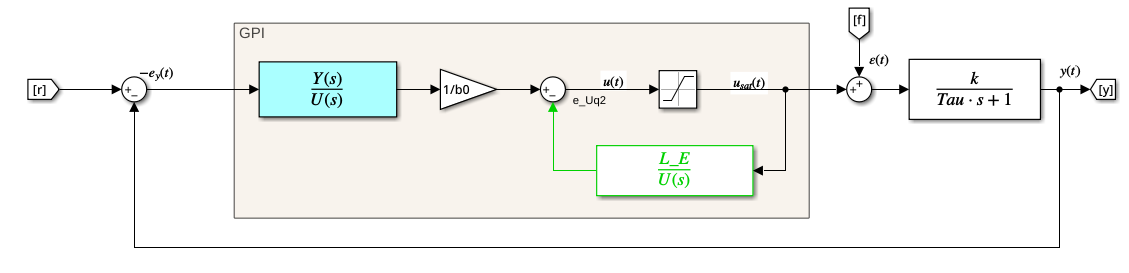
\includegraphics[width=\textwidth]{simulink_gpi_antiwindup.png}
  \caption[Implementación en Simulink del GPI con anti-windup]{Implementación en
    Simulink del GPI con realimentación de la saturación.}
  \label{fig:simulink_gpi}
\end{figure}

La Figura~\ref{fig:sat_arranque} compara el arranque desde $0$~mg/L con el soplador limitado. Sin
\emph{anti-windup}, el GPI se queda unos $16$~min en $100~\%$ y el oxígeno sube hasta $2{,}79$~mg/L;
con él, llega a la consigna sin pasarse, y con el polinomio del observador,
$E_1 = s^2 + l_1 s + l_2$, su respuesta se superpone a la del ADRC.

\begin{figure}[H]
  \centering
  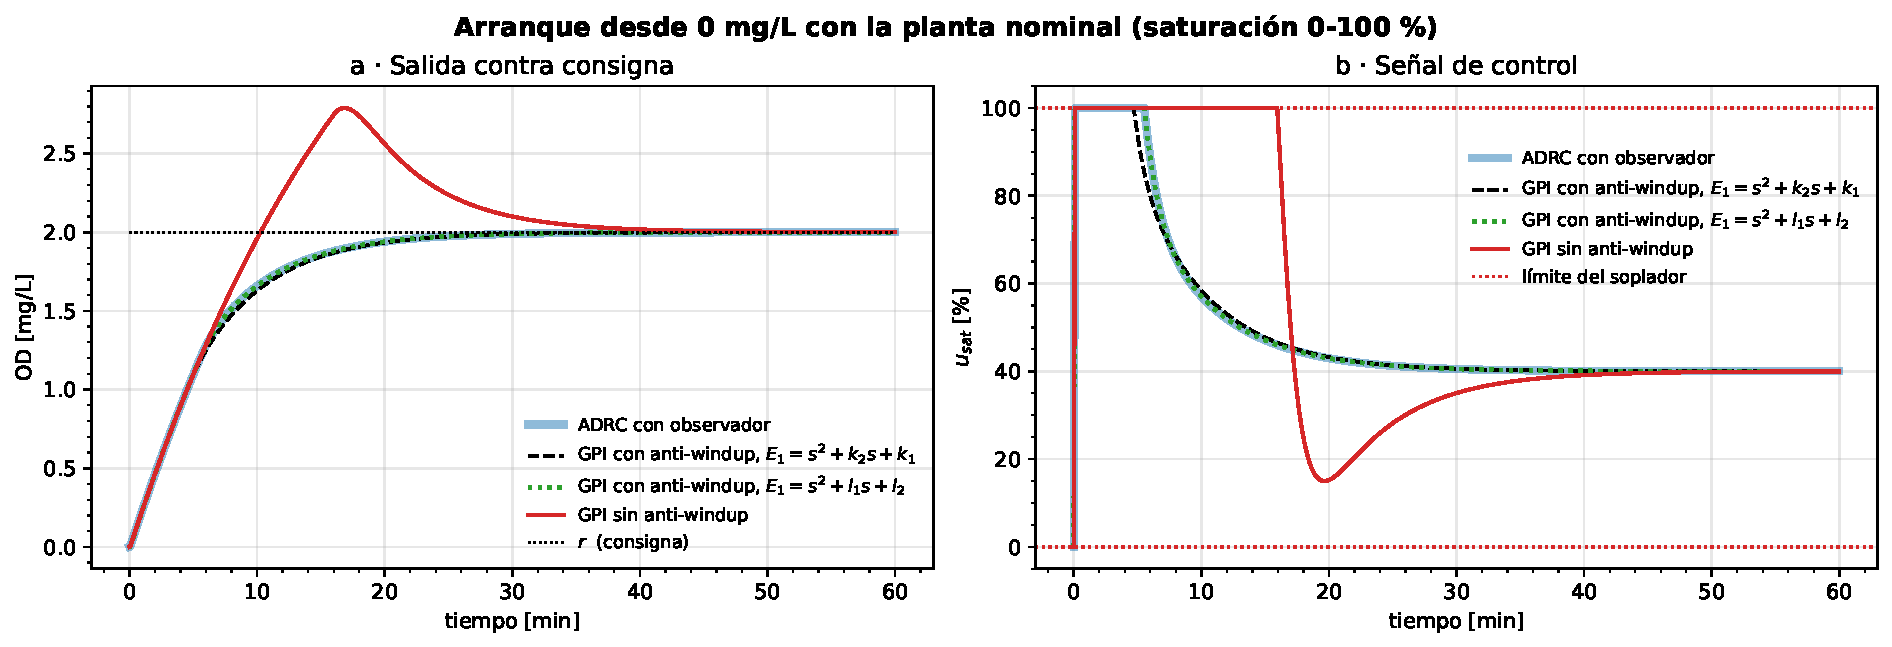
\includegraphics[width=\textwidth]{saturacion_arranque.pdf}
  \caption[Arranque desde cero con saturación]{Arranque desde $0$~mg/L con la
    planta nominal y el soplador limitado entre $0$ y $100~\%$: ADRC con
    observador, GPI con \emph{anti-windup} con $E_1 = s^2 + k_2 s + k_1$ y con
    el polinomio del observador, $E_1 = s^2 + l_1 s + l_2$, y GPI sin
    \emph{anti-windup}. (a) Salida contra consigna. (b) Señal de control.}
  \label{fig:sat_arranque}
\end{figure}

%--------------------------------------------------------------------
\subsection{Variación de los parámetros de la planta con saturación}
\label{subsec:sat_variacion}

Se repiten las variaciones de la Sección~\ref{subsec:caso_variacion} con el
soplador limitado entre $0$ y $100~\%$, para el GPI con realimentación de la
saturación \eqref{eq:aw_gpi} y las ganancias nominales
(Figura~\ref{fig:sat_adrc_gpi_variacion}). El ADRC con observador
(Sección~\ref{subsec:sat_adrc}) da prácticamente las mismas respuestas, así que
solo se muestra el GPI. Al retardo se le añade un caso
extremo, $\theta = 100$~s, el doble del de diseño y cerca del margen de retardo
de $110$~s (Sección~\ref{subsec:caso_margenes}): el oxígeno sube hasta
$2{,}42$~mg/L y el soplador llega a $100~\%$ y a $0~\%$, pero con la
realimentación de la saturación el controlador no se desestabiliza,
y la oscilación se amortigua lentamente. En caso de que la ganancia de la planta sea muy pequeña
(un cuarto de la nominal en la Figura~\ref{fig:sat_adrc_gpi_variacion}(a)), el controlador se
mantiene saturado, es decir, el sistema no llega a la referencia: con el soplador al $100~\%$ el
OD cae hasta $1{,}25$~mg/L; y cuando el controlador vuelva a
responder, la salida se irá acercando lentamente a la referencia a medida que el sistema se
recupere, sin sobrepicos agresivos ni enormes, gracias al \emph{anti-windup}.


\begin{figure}[H]
  \centering
  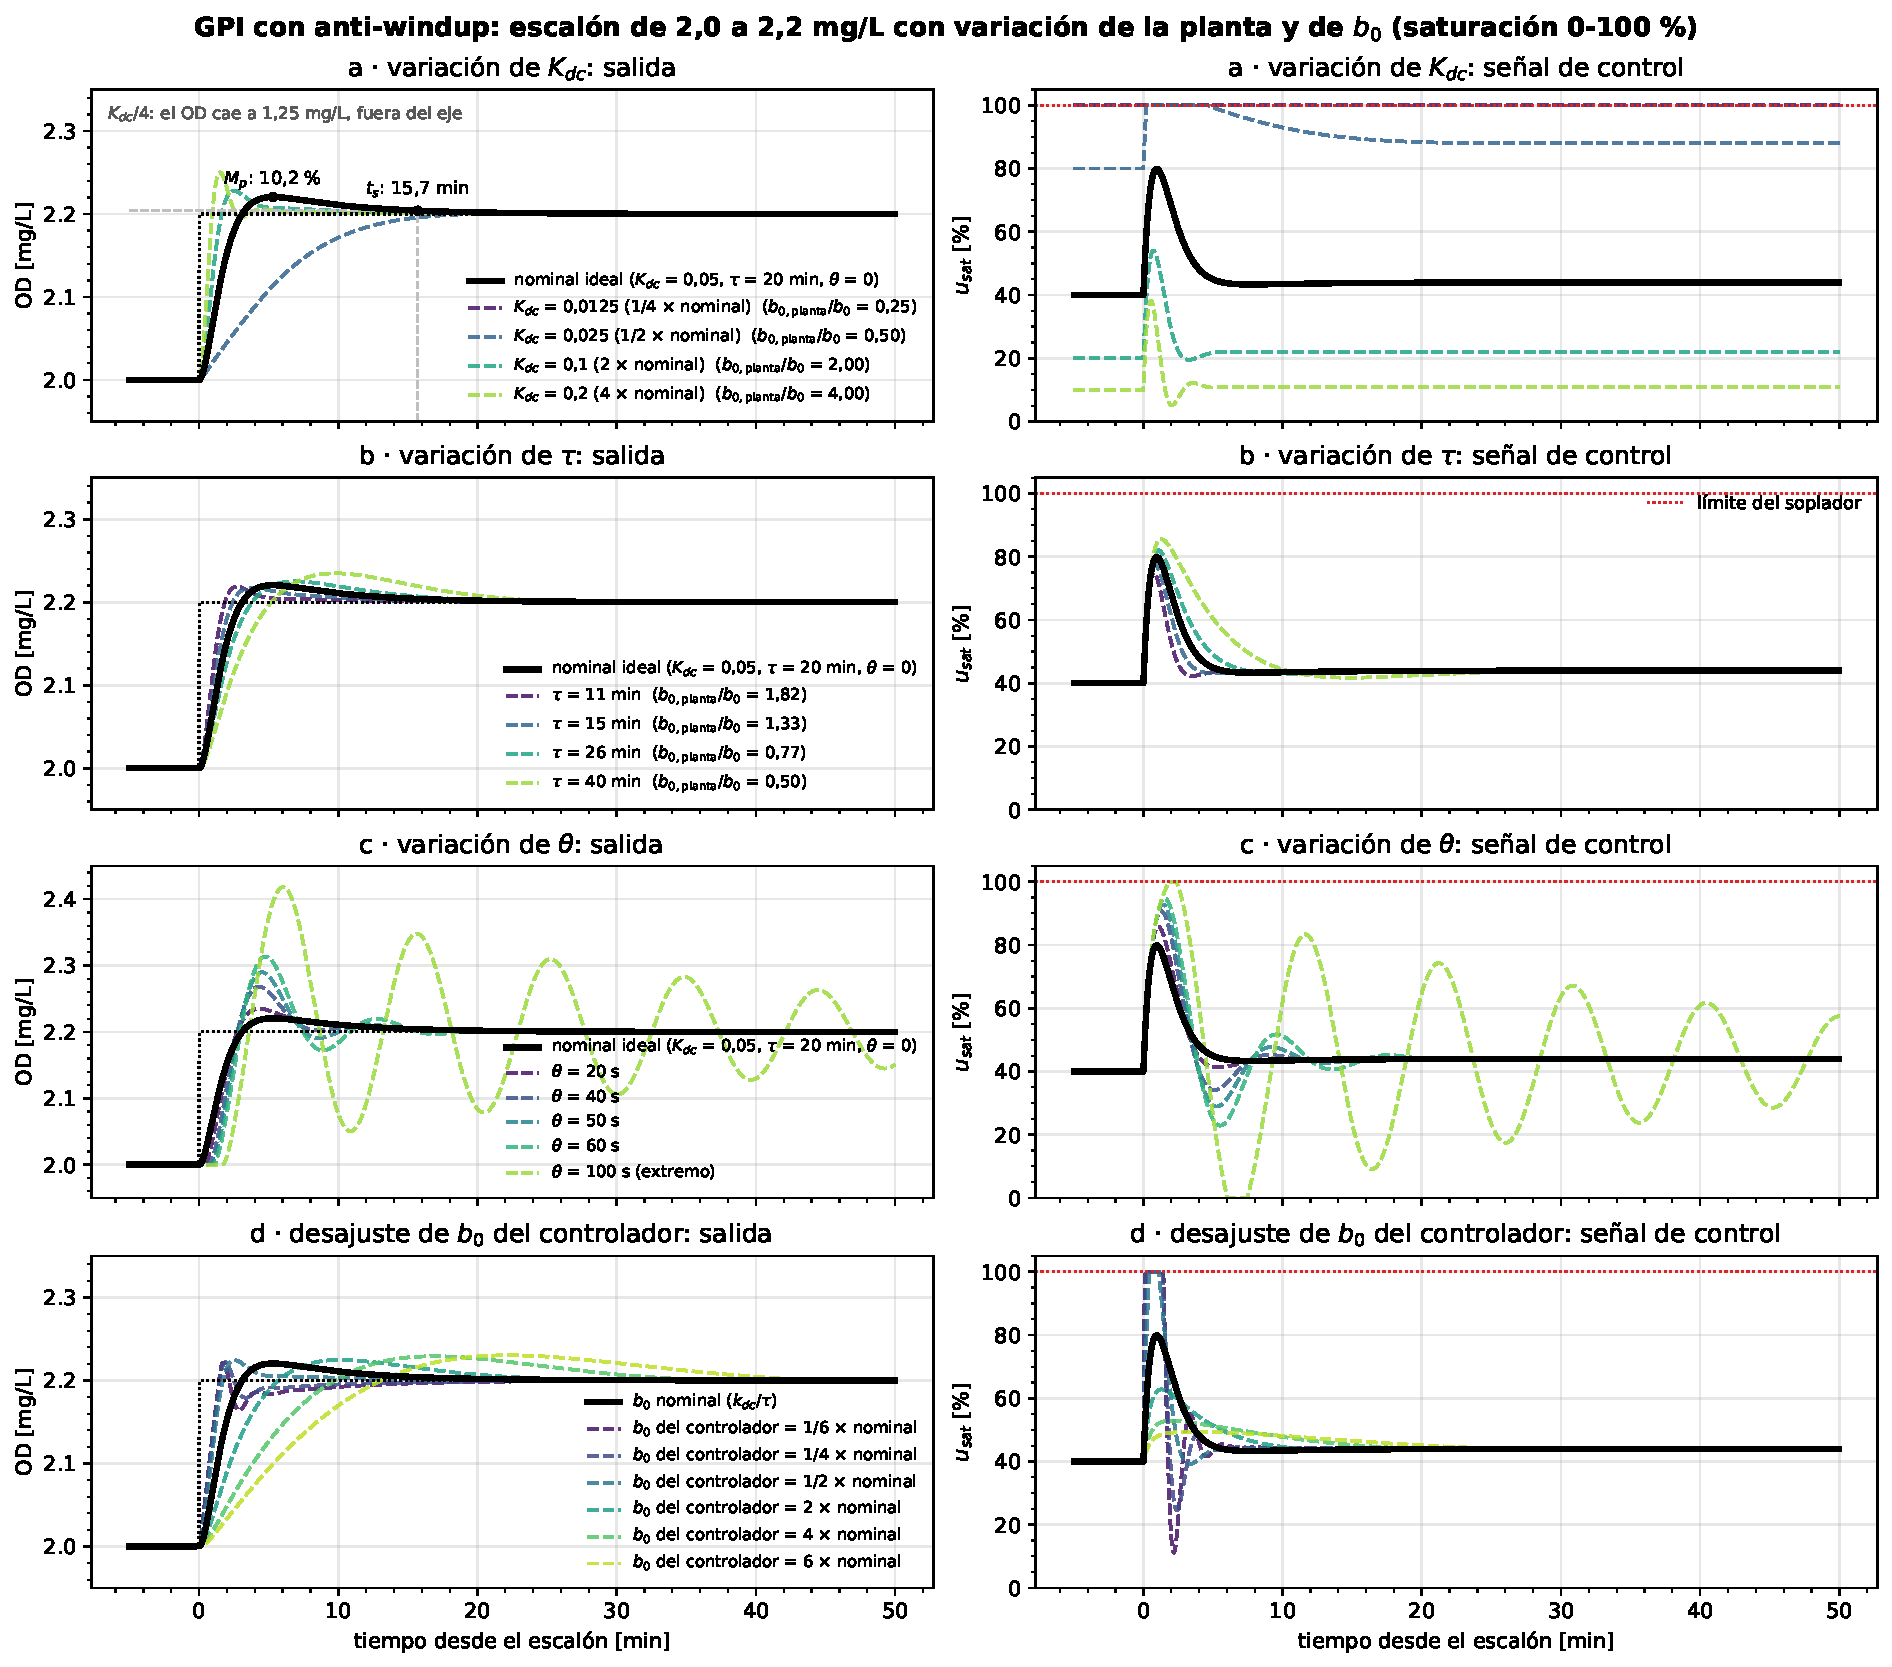
\includegraphics[width=\textwidth]{saturacion_adrc_gpi_variacion.pdf}
  \caption[GPI con saturación ante variaciones de la planta]{Escalón de
    consigna de $2{,}0$ a $2{,}2$~mg/L con el soplador limitado entre $0$ y
    $100~\%$ y el GPI con \emph{anti-windup} \eqref{eq:aw_gpi}, variando
    (a) $K_{dc}$, (b) $\tau$, (c) $\theta$, con un caso extremo de
    $\theta = 100$~s que satura el soplador, y (d) el $b_0$ del controlador. En
    negro, la planta nominal ideal, con $M_p$ y $t_s$ como en la Tabla~\ref{tab:metricas}.}
  \label{fig:sat_adrc_gpi_variacion}
\end{figure}



%--------------------------------------------------------------------
\section{Acondicionamiento de la referencia}
\label{sec:impl_referencia}

Ante un cambio de consigna, el ADRC basado en el error se pasa de la consigna aunque todos sus
polos sean reales (Sección~\ref{subsec:caso_variacion}). En el modelo de diseño (la cadena de
integradores), la respuesta a la consigna es
\begin{equation}
\frac{y}{r} = \frac{k_1 s + k_0}{s^3 + k_2 s^2 + k_1 s + k_0}
= \frac{k_1 s + k_0}{(s + \omega_c)\,(s + \omega_o)^2} .
\label{eq:pref_yr}
\end{equation}
Tiene tres polos, $-\omega_c$ (el del controlador) y $-\omega_o$ doble (el del observador), y un
cero en
\begin{equation}
s = -\frac{k_0}{k_1} = -\frac{\omega_c\,\omega_o}{\omega_o + 2\omega_c} = -\frac{5}{7}\,\omega_c ,
\end{equation}
más lento que el polo $-\omega_c$: ese cero es el que produce el sobrepico. Además, como se vio en
la Sección~\ref{subsec:caso_simulacion}, un escalón en la consigna pide un pico muy grande en la
señal de control, porque el controlador debe compensar $u^* = \dot{y}^*$, que es un impulso.

Las dos cosas se reducen acondicionando la referencia antes de que entre al lazo, de dos formas:
suavizándola con un polinomio de Bézier (Sección~\ref{subsec:impl_bezier}) o pasándola por un
prefiltro de primer orden (Sección~\ref{sec:impl_esfuerzo}). En ambos casos el controlador no cambia
y el rechazo de la perturbación sigue siendo el mismo.

%--------------------------------------------------------------------
\subsection{Polinomio de Bézier}
\label{subsec:impl_bezier}
Se presenta el esquema de la Figura~\ref{fig:lazo_bezier}, donde se muestra un
acondicionamiento previo de la señal de referencia: la entrada es suavizada por un
polinomio de Bézier \cite{sira2017adrc,abadi2024robust}, que se busca que inicie lento, es decir, con derivadas en cero,
y que termine lento, también con derivadas en cero.

\begin{figure}[H]
  \centering
  \begin{tikzpicture}[>=Stealth, thick, font=\small,
      blk/.style={draw, thick, minimum width=1.5cm, minimum height=0.9cm},
      suma/.style={draw, thick, circle, minimum size=0.45cm, inner sep=0pt}]
    % bloque de Bezier con la curva en S
    \node[blk, minimum width=1.7cm, minimum height=1.2cm] (bz) at (2.1,0) {};
    \draw[thin, gray, ->] ($(bz.center)+(-0.65,-0.42)$) -- ($(bz.center)+(0.68,-0.42)$);
    \draw[thin, gray, ->] ($(bz.center)+(-0.65,-0.42)$) -- ($(bz.center)+(-0.65,0.48)$);
    \draw[line width=1.1pt, domain=0:1, samples=40, variable=\x]
      plot ({-0.55+1.1*\x+2.1}, {-0.32+0.65*\x*\x*(3-2*\x)});
    \node[above=1pt of bz, font=\footnotesize] {Bézier};
    \node[suma] (sa) at (5.3,0) {};
    \node[blk] (Ca) at (8.0,0) {$C(s)$};
    \node[suma] (sb) at (10.1,0) {};
    \node[blk] (Ga) at (12.2,0) {$G(s)$};
    \draw[->] (0,0) node[above right] {$r(t)$} -- (bz.west);
    \draw[->] (bz.east) -- node[above, pos=0.4] {$y^*(t)$} (sa.west);
    \draw[->] (sa.east) -- node[above] {$-e_y(t)$} (Ca.west);
    \draw[->] (Ca.east) -- node[above] {$u(t)$} (sb.west);
    \draw[->] (sb |- 0,1.2) node[above] {$\varepsilon(t)$} -- (sb.north);
    \draw[->] (sb.east) -- (Ga.west);
    \node at ($(sb.west)+(-0.2,-0.25)$) {$+$};
    \node at ($(sb.north)+(0.25,0.2)$) {$+$};
    \draw[->] (Ga.east) -- (15.2,0) node[above left] {$y(t)$};
    \fill (14.5,0) circle (1.5pt);
    \draw[->] (14.5,0) -- (14.5,-1.2) -- (5.3,-1.2) -- (sa.south);
    \node at ($(sa.west)+(-0.2,0.25)$) {$+$};
    \node at ($(sa.south)+(-0.25,-0.2)$) {$-$};
  \end{tikzpicture}
  \caption[Lazo con acondicionamiento de la referencia]{Lazo de control por
    realimentación del error con acondicionamiento de la referencia: la
    consigna $r(t)$ pasa por el polinomio de Bézier y el lazo sigue $y^*(t)$,
    con $e_y = y - y^*$.}
  \label{fig:lazo_bezier}
\end{figure}

%--------------------------------------------------------------------
\subsubsection{Planificación de la referencia}
\label{subsec:bz_planificacion}
Ahora bien, para esto, la referencia lleva la salida desde $y_0$ hasta la consigna $y_f$, partiendo y
llegando en reposo. Como la planta es de primer orden, basta con que $y^*$ y
$\dot{y}^*$ sean continuas: dos condiciones en cada extremo y un polinomio de
grado 3,
\begin{equation}
\begin{aligned}
y^*(t) &= a_3 t^3 + a_2 t^2 + a_1 t + a_0 , \\
\dot{y}^*(t) &= 3a_3 t^2 + 2a_2 t + a_1 .
\end{aligned}
\label{eq:bz_pol}
\end{equation}
Evaluando en $t_0$ y $t_f$,
\begin{equation}
\underbrace{\begin{bmatrix} y^*(t_0) \\ \dot{y}^*(t_0) \\ y^*(t_f) \\ \dot{y}^*(t_f) \end{bmatrix}}_{\mathbf{y}_{t_0,t_f}}
=
\underbrace{\begin{bmatrix}
t_0^3 & t_0^2 & t_0 & 1 \\
3t_0^2 & 2t_0 & 1 & 0 \\
t_f^3 & t_f^2 & t_f & 1 \\
3t_f^2 & 2t_f & 1 & 0
\end{bmatrix}}_{\mathbf{A}_y}
\underbrace{\begin{bmatrix} a_3 \\ a_2 \\ a_1 \\ a_0 \end{bmatrix}}_{\mathbf{a}_y} ,
\qquad
\mathbf{y}_{t_0,t_f} = \begin{bmatrix} y_0 & 0 & y_f & 0 \end{bmatrix}^{\top} ,
\qquad
\mathbf{a}_y = \mathbf{A}_y^{-1}\,\mathbf{y}_{t_0,t_f} .
\label{eq:bz_sistema}
\end{equation}
Con $t_0 = 0$ y $\Delta = y_f - y_0$,
\begin{equation}
a_0 = y_0 , \qquad a_1 = 0 , \qquad a_2 = \frac{3\,\Delta}{t_f^2} , \qquad a_3 = -\frac{2\,\Delta}{t_f^3} ,
\label{eq:bz_cerrada}
\end{equation}
y con el tiempo normalizado $\tau = t/t_f \in [0, 1]$,
\begin{equation}
\left.
\begin{aligned}
y^*(t) &= y_0 + \Delta\,\tau^2\,(3 - 2\tau) , \\
\dot{y}^*(t) &= \frac{\Delta}{t_f}\,6\,\tau\,(1 - \tau) ,
\end{aligned}
\right\}
\qquad 0 \le t \le t_f ,
\label{eq:bz_normalizada}
\end{equation}
con $y^* = y_0$ para $t < t_0$ y $y^* = y_f$ para $t > t_f$. Es el polinomio de
Bézier de grado 3 con puntos de control $\{y_0,\, y_0,\, y_f,\, y_f\}$, y su
velocidad máxima, en $\tau = 1/2$, es
\begin{equation}
\dot{y}^*_{\max} = 1{,}5\,\frac{\Delta}{t_f} .
\label{eq:bz_vmax}
\end{equation}
Las ecuaciones \eqref{eq:bz_normalizada} son las que se programan dentro de un bloque
de PLC: solo es necesario obtener la normalización del tiempo $\tau$ y medir el
tiempo actual, que se obtienen fácilmente con un contador y el tiempo de muestreo.
%--------------------------------------------------------------------
\subsubsection{Cambio de consigna y replanificación}
\label{subsec:bz_replanificacion}
Seguidamente se plantea el caso en que el operario realiza un cambio de consigna
cuando el sistema va subiendo.
Si la consigna cambia en $t_c$, el nuevo tramo parte del estado de la referencia,
no de la medición, con $t_0 = 0$ y $\tau = (t - t_c)/t_f$:
\begin{equation}
y_c = y^*(t_c) , \qquad \dot{y}_c = \dot{y}^*(t_c) , \qquad \bar{\Delta} = y_f - y_c ,
\label{eq:bz_estado_c}
\end{equation}
\begin{equation}
\begin{bmatrix} y_c \\ \dot{y}_c \\ y_f \\ 0 \end{bmatrix}
=
\begin{bmatrix}
0 & 0 & 0 & 1 \\
0 & 0 & 1 & 0 \\
t_f^3 & t_f^2 & t_f & 1 \\
3t_f^2 & 2t_f & 1 & 0
\end{bmatrix}
\begin{bmatrix} a_3 \\ a_2 \\ a_1 \\ a_0 \end{bmatrix}
\quad\Longrightarrow\quad
\begin{aligned}
a_0 &= y_c , & a_1 &= \dot{y}_c , \\
a_2 &= \frac{3\bar{\Delta} - 2\,\dot{y}_c\,t_f}{t_f^2} , & a_3 &= \frac{-2\bar{\Delta} + \dot{y}_c\,t_f}{t_f^3} .
\end{aligned}
\label{eq:bz_sistema_c}
\end{equation}
Con $c_i = a_i\,t_f^{\,i}$,
\begin{equation}
c_1 = \dot{y}_c\,t_f , \qquad
c_2 = 3\bar{\Delta} - 2\,\dot{y}_c\,t_f , \qquad
c_3 = -2\bar{\Delta} + \dot{y}_c\,t_f ,
\label{eq:bz_c}
\end{equation}
y de forma compacta:
\begin{equation}
\left.
\begin{aligned}
y^*(\tau) &= y_c + \tau\,\bigl(c_1 + \tau\,(c_2 + \tau\,c_3)\bigr) , \\
\dot{y}^*(\tau) &= \frac{1}{t_f}\,\bigl(c_1 + \tau\,(2c_2 + 3\tau\,c_3)\bigr) ,
\end{aligned}
\right\}
\qquad 0 \le \tau \le 1 ,
\label{eq:bz_horner}
\end{equation}
con $y^* = y_f$ y $\dot{y}^* = 0$ para $\tau > 1$. Con $\dot{y}_c = 0$,
\eqref{eq:bz_c} da $c_1 = 0$, $c_2 = 3\bar{\Delta}$ y $c_3 = -2\bar{\Delta}$, que es
\eqref{eq:bz_cerrada}. En el PLC, $\tau = n\,T_s/t_f$, con $n$ los ciclos desde
el inicio del tramo; al cambiar la consigna se recalcula \eqref{eq:bz_c} y se
reinicia $n = 0$, y al salir de \texttt{RESET} se toma $y_c = y$ medido y
$\dot{y}_c = 0$.

%--------------------------------------------------------------------
\subsubsection{Simulación en lazo cerrado}
\label{subsec:bz_simulacion}
La Figura~\ref{fig:adrc_lazo_cerrado_bezier} muestra el comportamiento de la planta cuando
se usa una referencia más suave, como la de Bézier. En el panel (a), el transitorio de $0$ a
$2{,}0$~mg/L dura unos $48$~min (cerca de $2{,}4\,\tau$), el tiempo final elegido para esa
maniobra, y el cambio de consigna de $2{,}0$ a $2{,}2$~mg/L se hace con un tiempo final de
$1\,\tau$. Como el suavizado solo se aplica a la referencia, el rechazo de la perturbación
exógena es prácticamente igual. En el panel (b) se puede observar que el observador logra
estimar adecuadamente el error de seguimiento (por ser de alta ganancia), aunque no de forma
exacta, por lo que sí se
sigue la curva de Bézier a pesar de que el modelo interno no tiene ese polinomio. Finalmente,
la señal de control se mantiene por debajo del $62~\%$ (panel d), por lo que sí se ve
reflejada una disminución muy buena de la señal de control.

Ahora bien, la Figura~\ref{fig:adrc_bezier_retardo} muestra el comportamiento de la planta
cuando se involucran retardos. Sin el acondicionamiento de la referencia (panel a), el
sobrepico va aumentando a medida que crece $\theta$; pero cuando se usa Bézier (panel b),
las oscilaciones prácticamente desaparecen, y aunque haya retardo, la planta logra un
transitorio suave, sin oscilaciones grandes que puedan llegar a saturar el controlador.

\begin{figure}[H]
  \centering
  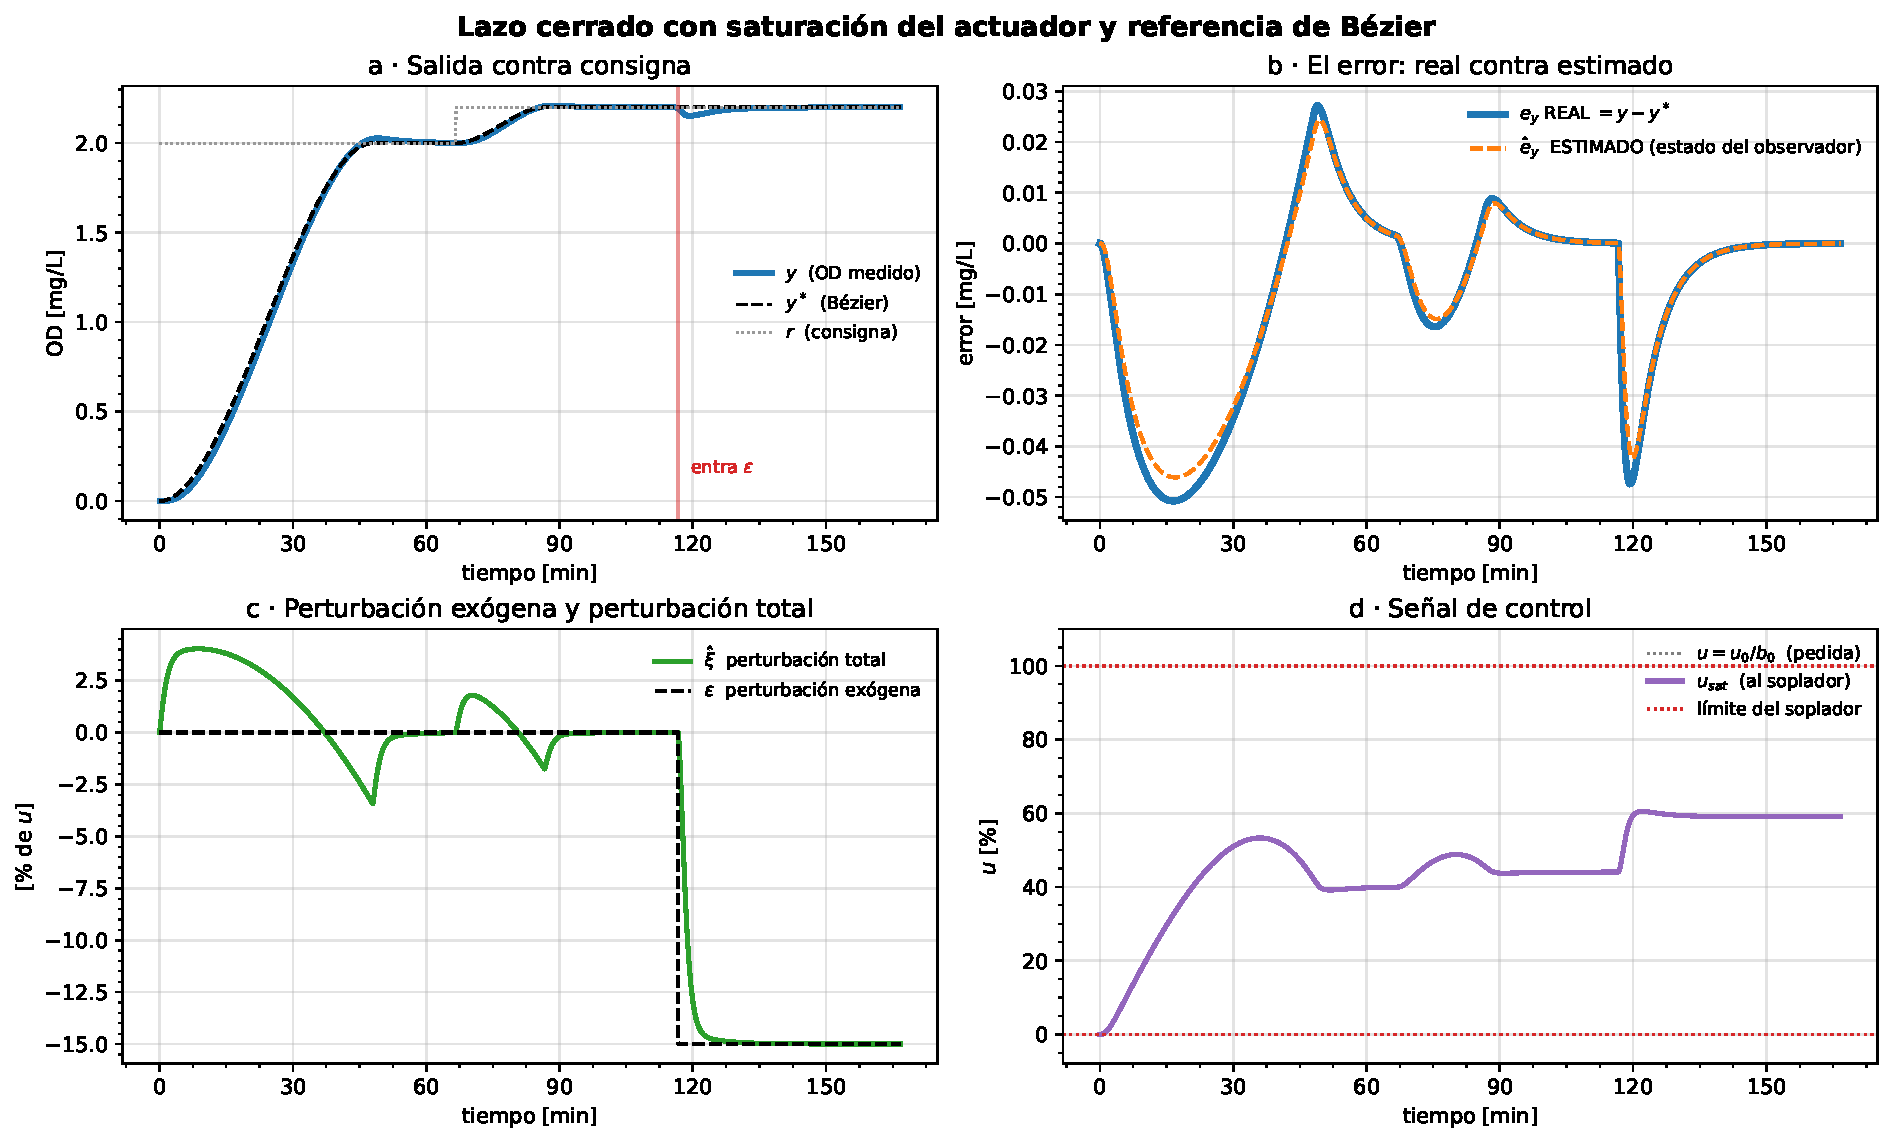
\includegraphics[width=\textwidth]{adrc_lazo_cerrado_bezier.pdf}
  \caption[Lazo cerrado del ADRC con referencia de Bézier]{Lazo cerrado del
    ADRC con la planta, el soplador limitado entre $0$ y $100~\%$ y la
    referencia de Bézier \eqref{eq:bz_normalizada}, en el mismo escenario de la
    Figura~\ref{fig:adrc_lazo_cerrado_saturacion}. (a) Salida contra la
    referencia $y^*$ y la consigna $r$. (b) Error de seguimiento real y
    estimado. (c) Perturbación exógena y perturbación total, en \% de $u$.
    (d) Orden pedida por el controlador y orden aplicada.}
  \label{fig:adrc_lazo_cerrado_bezier}
\end{figure}

\begin{figure}[H]
  \centering
  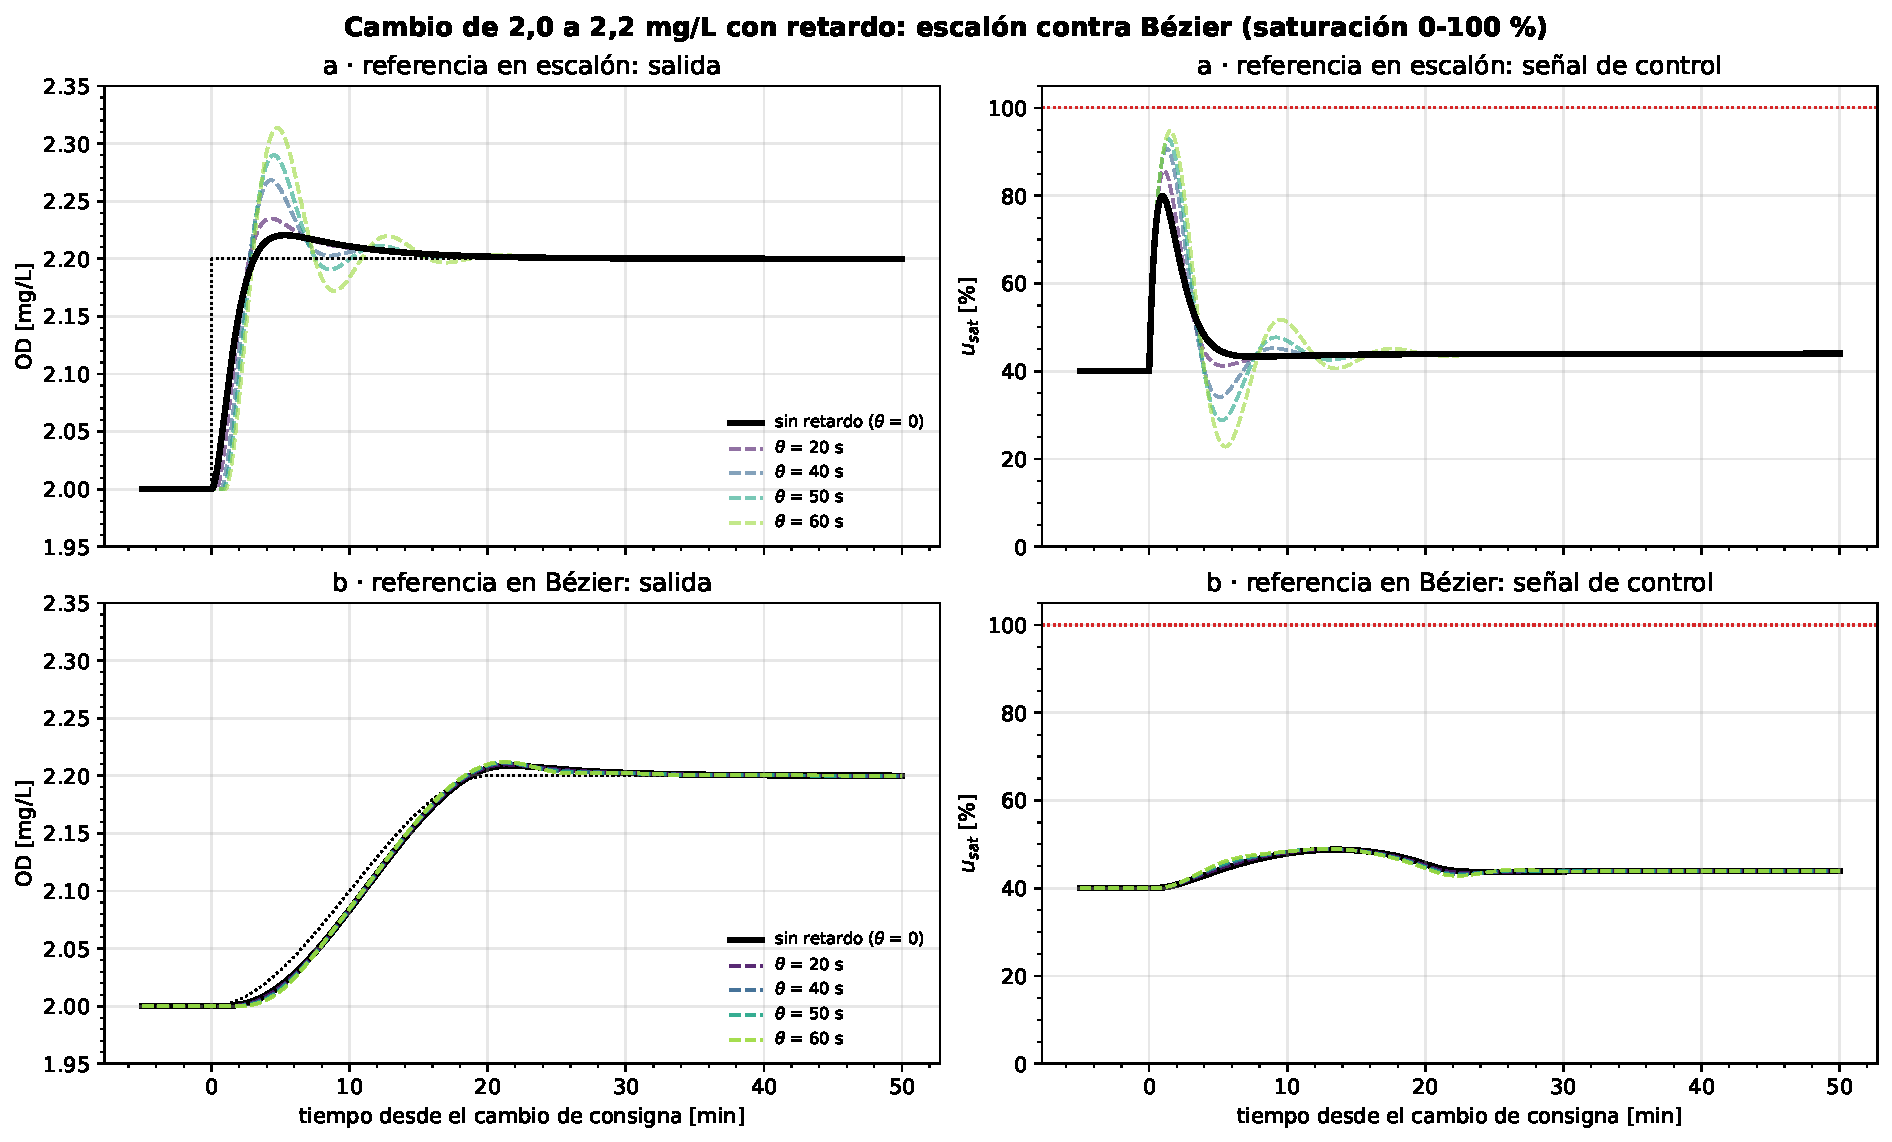
\includegraphics[width=\textwidth]{adrc_bezier_retardo.pdf}
  \caption[Escalón contra Bézier con retardo]{Cambio de consigna de $2{,}0$ a
    $2{,}2$~mg/L con la planta nominal, retardo $\theta$ en la entrada y el
    soplador limitado entre $0$ y $100~\%$: (a) consigna en escalón y
    (b) referencia de Bézier con $t_f = 20$~min. En negro, sin retardo.}
  \label{fig:adrc_bezier_retardo}
\end{figure}


%--------------------------------------------------------------------
\subsection{Prefiltro de consigna}
\label{sec:impl_esfuerzo}

Herbst y Madoński proponen agregar un prefiltro en el canal de la referencia del ADRC basado en
el error \cite[sec.~6.4.2]{herbst2024adrc}. Para quitar el cero de \eqref{eq:pref_yr}, aquí se pone
antes de la suma un prefiltro de primer orden con el polo justo en ese cero
(Figura~\ref{fig:pref_lazo}):
\begin{equation}
F(s) = \frac{k_0}{k_1 s + k_0} = \frac{1}{\dfrac{k_1}{k_0}\,s + 1}
= \frac{1}{\dfrac{\omega_o + 2\omega_c}{\omega_c\,\omega_o}\,s + 1} ,
\label{eq:pref_f}
\end{equation}
con ganancia estática $1$, para que la salida llegue a la consigna, y constante de tiempo
$k_1/k_0 = 420$~s ($7$~min). El prefiltro está fuera del lazo: el controlador no cambia y le sigue
entrando solo el error, ahora $e_y = y - r_f$.

\begin{figure}[H]
  \centering
  \begin{tikzpicture}[>=Stealth, thick, font=\small,
      blk/.style={draw, thick, minimum width=1.5cm, minimum height=0.9cm},
      suma/.style={draw, thick, circle, minimum size=0.45cm, inner sep=0pt}]
    \node[blk, minimum width=2.2cm, minimum height=1.1cm] (pf) at (2.2,0) {$\dfrac{k_0}{k_1 s + k_0}$};
    \node[above=1pt of pf, font=\footnotesize] {prefiltro};
    \node[suma] (sa) at (5.5,0) {};
    \node[blk] (Ca) at (8.0,0) {$C(s)$};
    \node[suma] (sb) at (10.5,0) {};
    \node[blk] (Ga) at (12.6,0) {$G(s)$};
    \draw[->] (0,0) node[above right] {$r(t)$} -- (pf.west);
    \draw[->] (pf.east) -- node[above] {$r_f(t)$} (sa.west);
    \draw[->] (sa.east) -- node[above] {$-e_y(t)$} (Ca.west);
    \draw[->] (Ca.east) -- node[above] {$u(t)$} (sb.west);
    \draw[->] (sb |- 0,1.2) node[above] {$\varepsilon(t)$} -- (sb.north);
    \draw[->] (sb.east) -- node[above] {$\bar{u}(t)$} (Ga.west);
    \draw[->] (Ga.east) -- (15.1,0) node[above left] {$y(t)$};
    \fill (14.4,0) circle (1.5pt);
    \draw[->] (14.4,0) -- (14.4,-1.2) -- (5.5,-1.2) -- (sa.south);
    \node at ($(sa.west)+(-0.2,0.25)$) {$+$};
    \node at ($(sa.south)+(-0.25,-0.2)$) {$-$};
    \node at ($(sb.west)+(-0.2,0.25)$) {$+$};
    \node at ($(sb.north)+(0.25,0.2)$) {$+$};
  \end{tikzpicture}
  \caption[Lazo con prefiltro de consigna]{Lazo de control con prefiltro de consigna, con
    $e_y = y - r_f$. El prefiltro está fuera del lazo.}
  \label{fig:pref_lazo}
\end{figure}

Con el prefiltro, el polo se cancela con el cero en \eqref{eq:pref_yr} y quedan los tres polos del
diseño, sin cero:
\begin{equation}
\begin{aligned}
\frac{y}{r} &= \frac{k_0}{k_1 s + k_0}\cdot\frac{k_1 s + k_0}{s^3 + k_2 s^2 + k_1 s + k_0} \\[4pt]
&= \frac{k_0}{s^3 + k_2 s^2 + k_1 s + k_0} = \frac{k_0}{(s + \omega_c)\,(s + \omega_o)^2} .
\end{aligned}
\label{eq:pref_yr_f}
\end{equation}
La respuesta a la perturbación no pasa por el prefiltro, así que sigue siendo la misma. En el
modelo de diseño, la perturbación total $\bar{\xi}$ entra a la cadena de integradores junto con $u_0$, y
\begin{equation}
\frac{y}{\bar{\xi}} = \frac{s\,(s + k_2)}{s^3 + k_2 s^2 + k_1 s + k_0}
= \frac{s\,(s + k_2)}{(s + \omega_c)\,(s + \omega_o)^2} ,
\label{eq:pref_rechazo}
\end{equation}
que no tiene ese cero y no cambia con $F(s)$. Es decir, el filtro solo se ve en el seguimiento de
la referencia y no en el rechazo de la perturbación.

En el escalón de $2{,}0$ a $2{,}2$~mg/L con la planta (Figura~\ref{fig:pref_escalon}), sin
retardo el prefiltro quita el sobrepico ($10{,}2$ a $0~\%$), baja el pico de $u$ de $80$ a $50~\%$
y la energía de la señal de control $E_u$ (Tabla~\ref{tab:metricas}) de $126\,544$ a $12\,209~\%^2\cdot$s. Con
$\theta = 50$~s el sobrepico baja de $44{,}6$ a $0~\%$, el pico de $u$ de $93$ a $54~\%$ y $E_u$ de $286\,035$ a
$19\,036~\%^2\cdot$s. A
cambio llega más tarde: entra a la banda de $2~\%$ en $24{,}4$~min en vez de $15{,}7$ sin retardo, y
en $24{,}7$ en vez de $14{,}7$ con $\theta = 50$~s. La perturbación de $-15~\%$ da la misma caída con
y sin prefiltro: el oxígeno baja hasta $2{,}15$~mg/L sin retardo y hasta $2{,}13$~mg/L con
$\theta = 50$~s.

\begin{figure}[tbp]
  \centering
  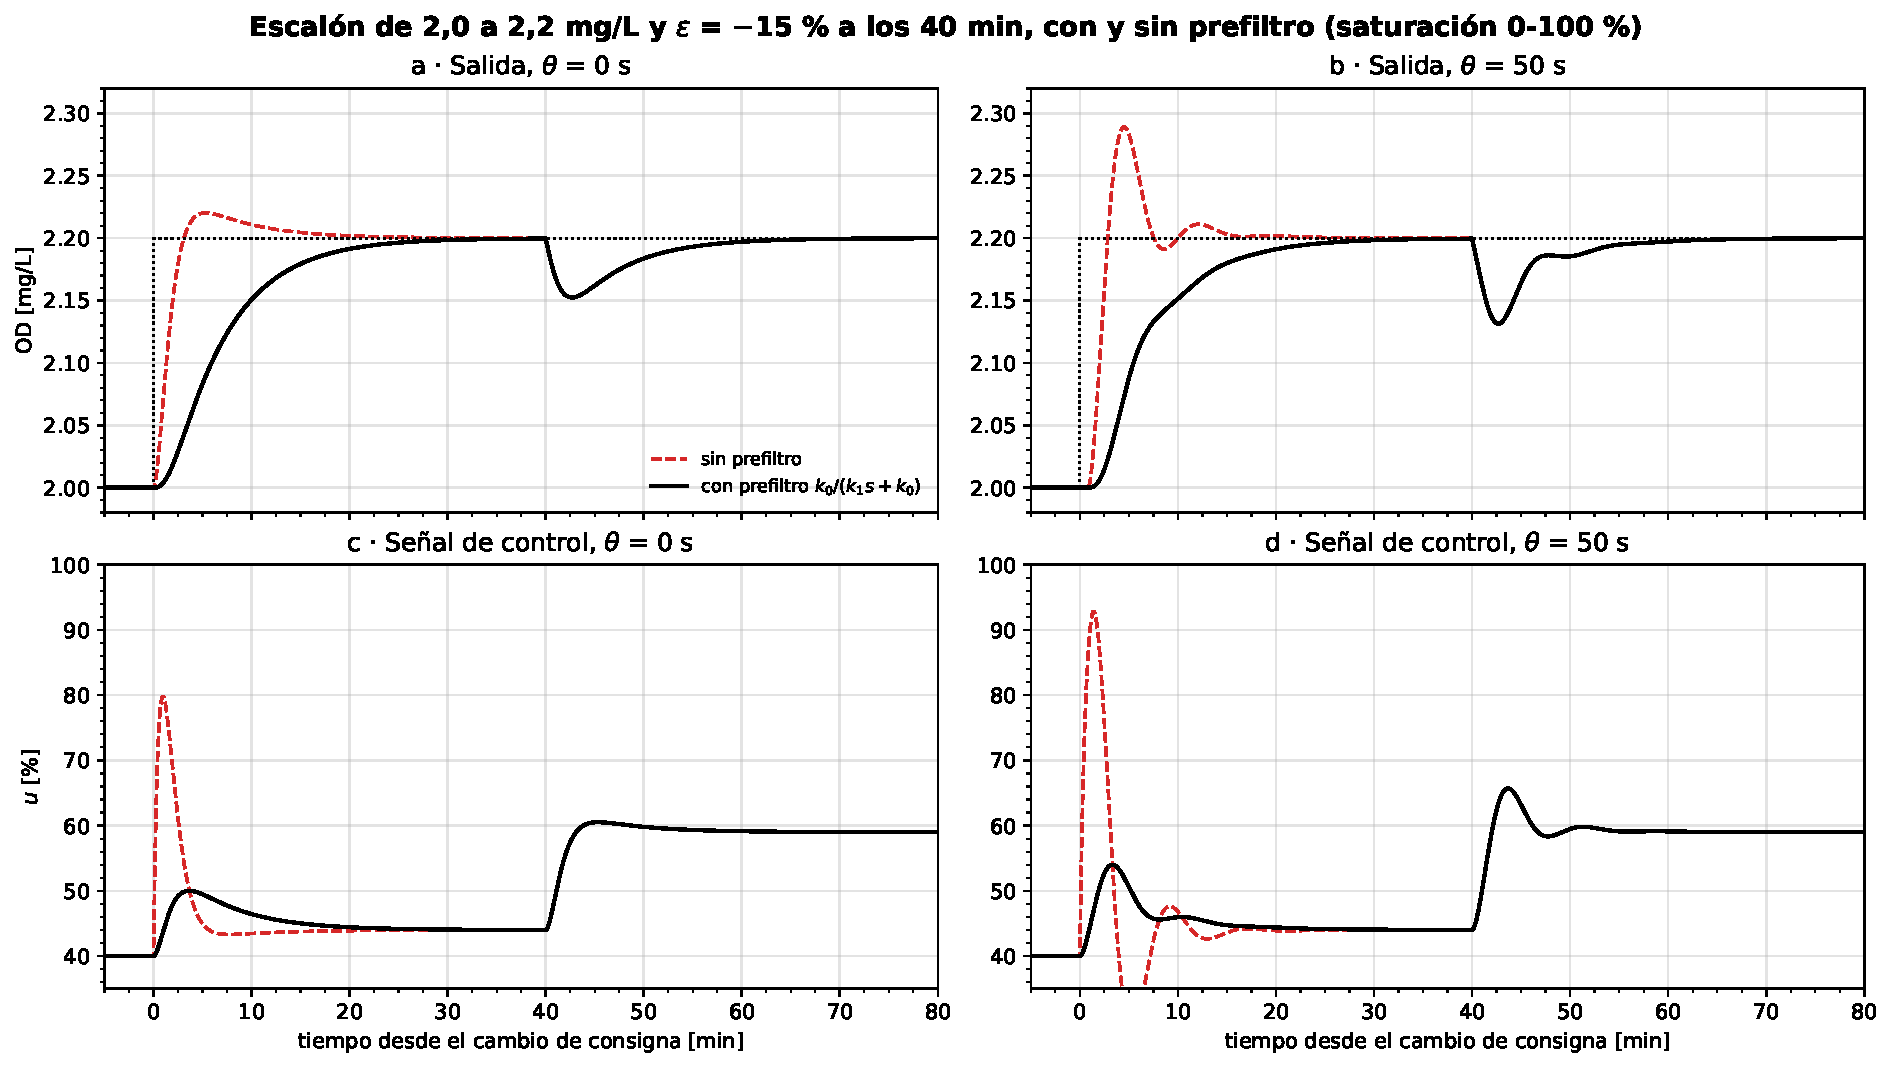
\includegraphics[width=\textwidth]{adrc_prefiltro.pdf}
  \caption[Escalón de consigna y perturbación con y sin prefiltro]{Escalón de consigna de
    $2{,}0$ a $2{,}2$~mg/L y perturbación $\varepsilon = -15~\%$ a los $40$~min, con la planta
    y el soplador limitado entre $0$ y $100~\%$, sin prefiltro y con el prefiltro
    \eqref{eq:pref_f}. (a) y (c) Sin retardo; (b) y (d) con $\theta = 50$~s. Arriba, la salida;
    abajo, la señal de control.}
  \label{fig:pref_escalon}
\end{figure}
Si se llega a cambiar la estructura del controlador, para seguir otro tipo de referencias, como
una rampa, o por el orden de la planta, es necesario reajustar el filtro según la estructura del
controlador, para anular los ceros del numerador de $y/r$. No es una regla exacta: poniendo un
filtro libre se pueden obtener buenos resultados suavizando la referencia, como en el ejemplo de
Herbst y Madoński \cite[sec.~6.4.2]{herbst2024adrc}; pero si se quiere la dinámica exacta del
diseño, sí es necesario reajustar el filtro con polos que cancelen los ceros del lazo cerrado. Además, con
referencias más suaves el prefiltro deja de ser necesario.

%--------------------------------------------------------------------
\section{Manejo del ruido}
\label{sec:impl_ruido}

Chen clasifica las funciones de transferencia según lo que hacen en alta frecuencia, y eso es lo que
decide cómo tratan el ruido. Una función de transferencia es estrictamente propia si $G(\infty) = 0$,
bipropia si $G(\infty)$ es finito y distinto de cero, e impropia si
$G(\infty) = \infty$ \cite[sec.~2.4]{chen1993analog}. Las impropias amplifican
el ruido de alta frecuencia, como un derivador, y las estrictamente propias lo
atenúan, como un integrador \cite[pp.~31--32]{chen1993analog}; por eso todo
compensador debe ser al menos propio \cite[sec.~6.5]{chen1993analog}.

El ruido $n$ de la medida llega al error y al soplador por las funciones de transferencia de la
Tabla~\ref{tab:caso_gang}:
\begin{equation}
\frac{-e_y}{n} = \frac{-1}{1 + CG},
\qquad
\frac{u}{n} = \frac{-C}{1 + CG} .
\label{eq:ruido_ft}
\end{equation}
Por encima del ancho de banda, con $C$ bipropio el
ruido pasa al soplador con la ganancia $C(\infty)$ hasta la frecuencia de
Nyquist; con $C$ estrictamente propio, se atenúa.

El GPI \eqref{eq:gpi_pi_filtro} es estrictamente propio: su ganancia cae como
$1/\omega$ y tiende a cero,
\begin{equation}
C_{GPI}(s) = \frac{1}{b_0}\,\frac{k_1 s + k_0}{s\,(s + k_2)},
\qquad
|C_{GPI}(j\omega)| \xrightarrow{\;\omega \to \infty\;} \frac{k_1}{b_0\,\omega} \to 0,
\qquad
C_{GPI}(\infty) = 0 .
\end{equation}
Sin el filtro, con su
ganancia estática $1/k_2$, queda el PI bipropio clásico, cuya ganancia tiende a
una constante:
\begin{equation}
C_{PI}(s) = \frac{1}{b_0 k_2}\,\frac{k_1 s + k_0}{s},
\qquad
C_{PI}(\infty) = \frac{k_1}{b_0 k_2} = 254{,}5~\%/(\mathrm{mg/L}) .
\end{equation}
El ruido en el error llega casi el mismo con los dos controladores, pero en $u$ el PI se queda en
$48{,}1$~dB hasta Nyquist y el GPI cae $20$~dB/década
(Figura~\ref{fig:ruido_gpi_vs_pi}). Simulados con el ruido del sensor
(Sección~\ref{sec:ident_ruido}), $\sigma_u$ da $0{,}0080~\%$ con el GPI y
$0{,}28~\%$ con el PI, $35$ veces más: el PI deja pasar mucho más ruido a la señal de control. En
el escalón del
Capítulo~\ref{cap:comparacion_pid} pasa lo mismo con el PID ISA, también
bipropio: $0{,}22~\%$ frente a $0{,}009~\%$ del ADRC
(Figura~\ref{fig:pid_adrc_escalon},
Tabla~\ref{tab:pid_escalon}).

\begin{figure}[H]
  \centering
  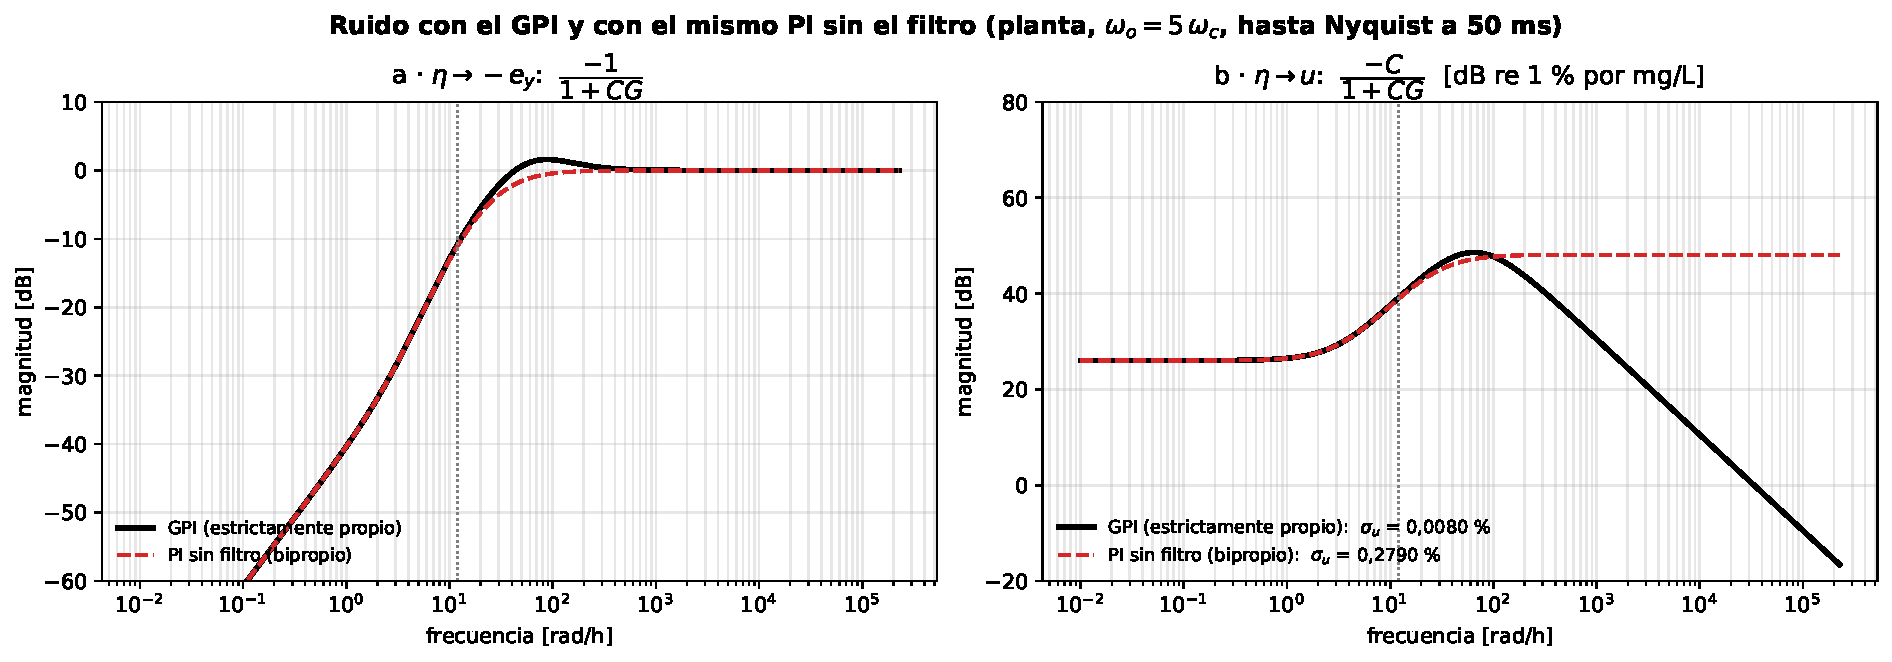
\includegraphics[width=\textwidth]{ruido_gpi_vs_pi.pdf}
  \caption[Ruido con el GPI y con el PI sin filtro]{Funciones de transferencia
    del ruido \eqref{eq:ruido_ft} con la planta y $\omega_o = 5\,\omega_c$,
    hasta la frecuencia de Nyquist a $50$~ms: GPI (estrictamente propio) y el
    mismo PI sin el filtro (bipropio). (a) Hacia $-e_y$. (b) Hacia $u$, con la
    $\sigma_u$ simulada con el ruido del sensor. La vertical marca $\omega_c$.}
  \label{fig:ruido_gpi_vs_pi}
\end{figure}

Herbst y Madoński presentan la misma idea: el controlador del ADRC, que es el mismo en el enfoque
basado en el error, es estrictamente propio \cite[ecs.~4.20 y 6.30]{herbst2024adrc}, y el máximo de
$\omega_o$ lo pone el ruido admisible en $u$.  Es decir, al pasar de $\omega_o = 5\,\omega_c$ a
$10\,\omega_c$, el ruido llega al soplador con $3{,}4$ veces más ganancia
(Figura~\ref{fig:adrc_gang_kESO}(h)). Con $\omega_o = 5\,\omega_c$ y un
controlador estrictamente propio no hacen falta filtros adicionales. Por ende, con el ADRC, ya sea basado en
observador de estado extendido o en su forma GPI, se puede ajustar el ruido admisible con el ancho de banda
del observador, $\omega_o$. Por ende, el ajuste de $\omega_o$ dependerá de
las frecuencias de las perturbaciones que se desean rechazar y del tope máximo de ruido admisible
que se deja pasar a la señal de control.

%--------------------------------------------------------------------
\section{Discretización}
\label{sec:impl_discretizacion}

En el PLC el controlador es un sistema digital: el error se muestrea con un
conversor A/D, el controlador discreto $C(z)$ calcula la orden en cada periodo de
muestreo $T_s$, y un conversor D/A la mantiene constante hasta la muestra
siguiente (Figura~\ref{fig:lazo_digital}) \cite[sec.~12.1]{chen1993analog}.

\begin{figure}[H]
  \centering
  \begin{tikzpicture}[>=Stealth, thick, font=\small,
      blk/.style={draw, thick, minimum width=1.3cm, minimum height=0.9cm},
      suma/.style={draw, thick, circle, minimum size=0.45cm, inner sep=0pt}]
    \node[suma] (sa) at (1.6,0) {};
    \node[blk] (ad) at (3.9,0) {A/D};
    \node[blk, minimum width=1.6cm] (cz) at (6.5,0) {$C(z)$};
    \node[blk] (da) at (9.1,0) {D/A};
    \node[blk, minimum width=1.6cm] (gs) at (11.7,0) {$G(s)$};
    \node[blk, minimum width=1.5cm, minimum height=0.6cm] (ck) at (6.5,-1.05) {reloj};
    \draw[->] (0,0) node[above right] {$r(t)$} -- (sa.west);
    \draw[->] (sa.east) -- node[above] {$-e_y(t)$} (ad.west);
    \draw[->] (ad.east) -- node[above] {$-e_y[k]$} (cz.west);
    \draw[->] (cz.east) -- node[above] {$u[k]$} (da.west);
    \draw[->] (da.east) -- node[above] {$u(t)$} (gs.west);
    \draw[->] (gs.east) -- (14.4,0) node[above left] {$y(t)$};
    \fill (13.7,0) circle (1.5pt);
    \draw[->] (13.7,0) -- (13.7,-1.75) -- (1.6,-1.75) -- (sa.south);
    \draw[->] (ck.west) -- (ad |- ck) -- (ad.south);
    \draw[->] (ck.east) -- (da |- ck) -- (da.south);
    \draw[->] (ck.north) -- (cz.south);
    \node at ($(sa.west)+(-0.2,0.25)$) {$+$};
    \node at ($(sa.south)+(-0.25,-0.2)$) {$-$};
  \end{tikzpicture}
  \caption[Lazo de control digital]{Lazo de control digital, con
    $e_y = y - r$ \cite[fig.~12.1]{chen1993analog}.}
  \label{fig:lazo_digital}
\end{figure}

Las técnicas de realimentación de estado y de estimadores del caso continuo se
aplican sin modificaciones al discreto; la diferencia es que los polos deseados
se ubican dentro del círculo unitario \cite[sec.~13.7]{chen1993analog}.

\paragraph{Métodos de discretización.} El controlador continuo,
$C(s) = \frac{1}{b_0}\frac{k_1 s + k_0}{s\,(s + k_2)}$, se puede llevar a $C(z)$ con
\begin{equation}
\begin{gathered}
\text{ZOH: } C(z) = (1 - z^{-1})\,\mathcal{Z}\!\left\{\frac{C(s)}{s}\right\},
\qquad
\text{Tustin: } s \to \frac{2}{T_s}\,\frac{z - 1}{z + 1},\\[4pt]
\text{Euler hacia adelante: } s \to \frac{z - 1}{T_s},
\qquad
\text{Euler hacia atrás: } s \to \frac{z - 1}{T_s\,z},
\end{gathered}
\label{eq:disc_metodos}
\end{equation}
o diseñarse directamente en discreto (Sección~\ref{subsec:disc_adrc}). La
Figura~\ref{fig:disc_metodos_bode} compara sus respuestas en frecuencia,
evaluadas en $z = e^{j\omega T_s}$ hasta la frecuencia de Nyquist, $\pi/T_s$.

\begin{figure}[H]
  \centering
  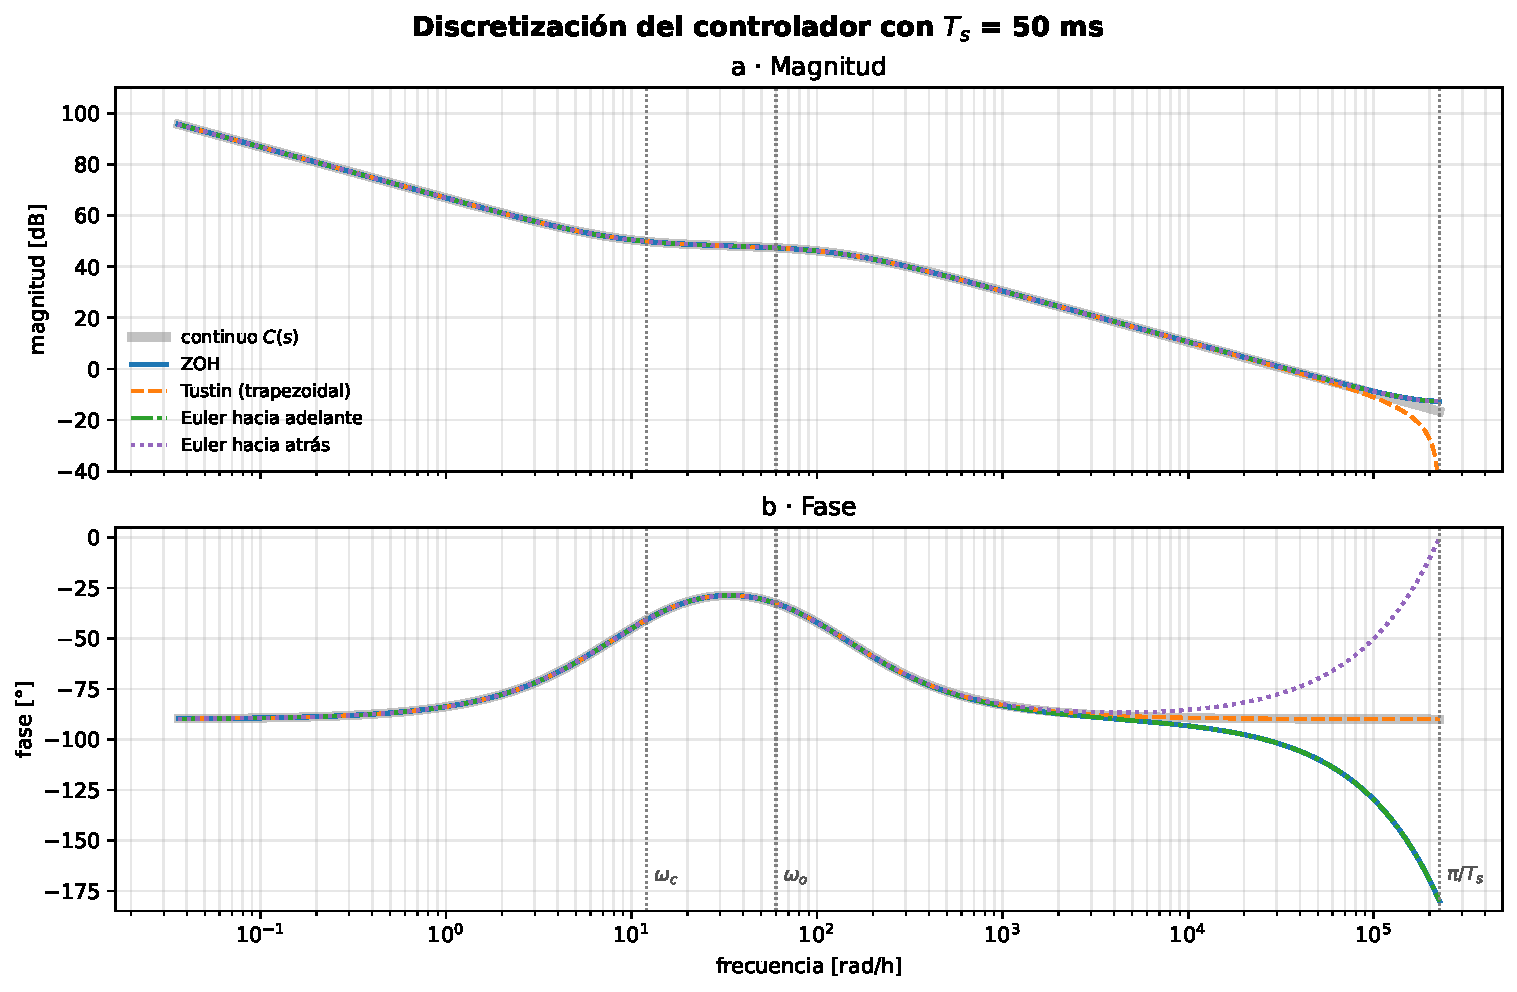
\includegraphics[width=0.85\textwidth]{disc_metodos_bode.pdf}
  \caption[Discretización del controlador por distintos métodos]{Respuesta en
    frecuencia del controlador continuo $C(s)$ y de sus versiones discretas con
    $T_s = 50$~ms: ZOH, Tustin, Euler hacia adelante y Euler hacia atrás.
    (a) Magnitud y (b) fase; las verticales
    marcan $\omega_c$, $\omega_o$ y la frecuencia de Nyquist $\pi/T_s$.}
  \label{fig:disc_metodos_bode}
\end{figure}

En la Figura~\ref{fig:disc_metodos_bode} se observa que, hasta unos
$10^4$~rad/h, todas las curvas prácticamente coinciden con la del controlador
continuo, y que las frecuencias $\omega_o$ y $\omega_c$ se encuentran alejadas
en más de dos décadas de ese valor. Por lo tanto, en este caso se obtiene un buen
resultado sin importar el método de discretización que se use. Esto se debe
directamente al tiempo de muestreo, ya que la planta es muy lenta comparada con
él. Chen menciona que el muestreo debe ser, como mínimo, unas 10 veces el ancho
de banda del lazo cerrado, recomienda unas 20 veces, y concluye que, si el periodo
es suficientemente pequeño, cualquier método sirve para discretizar un
compensador analógico
\cite[sec.~13.3.1]{chen1993analog}. El ancho de banda del lazo cerrado con la planta es de
$56{,}4$~rad/h, y la frecuencia de muestreo,
$\omega_s = 2\pi/T_s = 125{,}7$~rad/s, es decir,
$4{,}52\times10^{5}$~rad/h, queda casi cuatro órdenes de magnitud por encima. Si
se muestreara a 10 veces el ancho de banda del lazo cerrado, se tendría
$\omega_s = 564$~rad/h, es decir, un tiempo de muestreo de $40$~s; con este
valor de $T_s$ se obtiene la Figura~\ref{fig:disc_metodos_bode_40}. Se observa
que, en las frecuencias del lazo de control, las magnitudes se mantienen juntas,
mientras que en la fase algunos métodos empiezan a separarse del continuo. El
método que mantuvo un comportamiento más parecido al continuo, en magnitud y en
fase, a la frecuencia del lazo cerrado es Tustin: en el cruce de ganancia se separa
$0{,}13^{\circ}$, frente a $1^{\circ}$ a $3^{\circ}$ de Euler y casi $17^{\circ}$ de ZOH.

\begin{figure}[H]
  \centering
  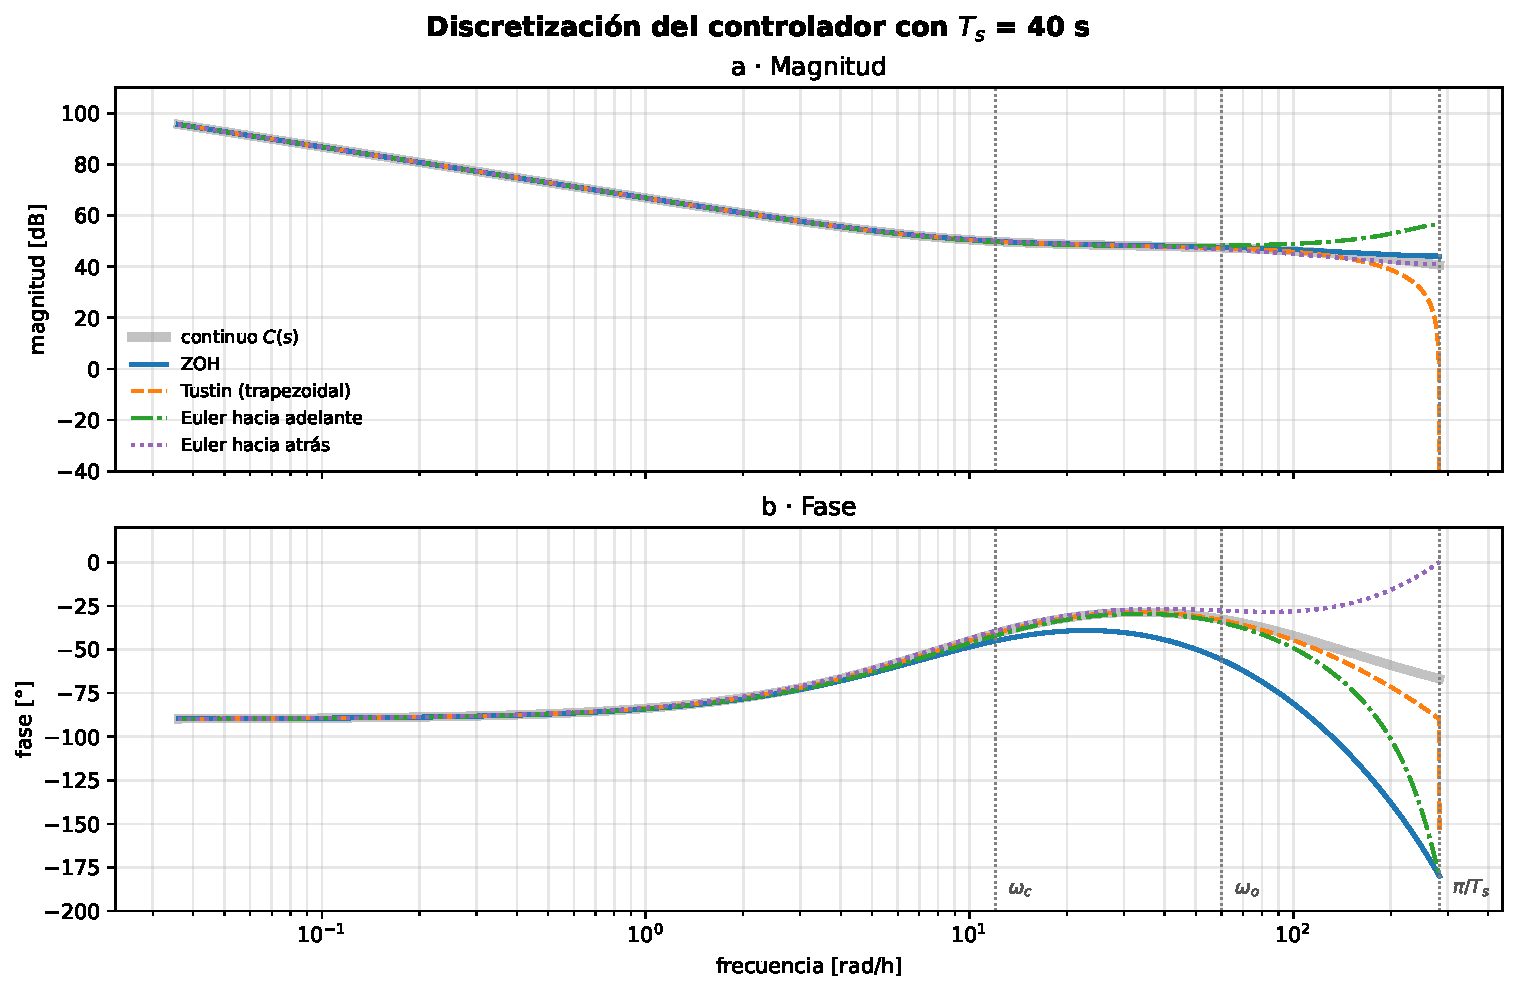
\includegraphics[width=0.85\textwidth]{disc_metodos_bode_40s.pdf}
  \caption[Discretización del controlador con $T_s = 40$~s]{Respuesta en
    frecuencia del controlador continuo $C(s)$ y de sus versiones discretas con
    $T_s = 40$~s, 10 veces el ancho de banda del lazo cerrado: ZOH, Tustin,
    Euler hacia adelante y Euler hacia atrás. (a) Magnitud y (b) fase; las
    verticales marcan $\omega_c$,
    $\omega_o$ y la frecuencia de Nyquist $\pi/T_s$.}
  \label{fig:disc_metodos_bode_40}
\end{figure}

%--------------------------------------------------------------------
\subsection{ADRC basado en observador de estado}
\label{subsec:disc_adrc}

El controlador se ejecuta cada $T_s = 50$~ms: el conversor A/D muestrea el
error y el conversor D/A mantiene la orden aplicada constante entre muestras,
como un retenedor de orden cero (ZOH). El modelo de diseño se discretiza con el
mismo retenedor (Figura~\ref{fig:adrc_discreto}).

\begin{figure}[H]
  \centering
  \resizebox{\textwidth}{!}{%
  \begin{tikzpicture}[>=Stealth, thick, font=\small,
      blk/.style={draw, thick, minimum width=1.3cm, minimum height=0.9cm},
      suma/.style={draw, thick, circle, minimum size=0.45cm, inner sep=0pt}]
    \node[suma] (sa) at (3.2,0) {};

    % --- ADRC discreto: observador, ley de control y saturacion ---
    \node[block, minimum width=6.0cm, minimum height=1.9cm] (obs) at (8.9,-0.4)
      {$\mathbf{A}_o\widehat{\mathbf{X}}[k] + \mathbf{B}_o \mathbf{u}_t[k]$ \\[10pt]
       $\mathbf{C}_o\widehat{\mathbf{X}}[k] + \mathbf{D}_o \mathbf{u}_t[k]$};
    \node[above=2pt of obs] {Observador discreto};
    \node[block, minimum size=9mm] (K) at (13.8,0) {$-\mathbf{K}_d$};
    \coordinate (u0) at (15.3,0);
    \node[block, minimum size=9mm] (ib) at (16.7,0) {$1/b_0$};
    \node[block, minimum size=11mm] (sat) at (19.0,0) {};
    \draw[thin, gray] ($(sat.center)+(-0.38,0)$) -- ($(sat.center)+(0.38,0)$);
    \draw[thin, gray] ($(sat.center)+(0,-0.38)$) -- ($(sat.center)+(0,0.38)$);
    \draw[line width=1.1pt] ($(sat.center)+(-0.38,-0.22)$) -- ($(sat.center)+(-0.18,-0.22)$)
                         -- ($(sat.center)+(0.18,0.22)$) -- ($(sat.center)+(0.38,0.22)$);
    \node[above=2pt of sat, font=\footnotesize] {0--100~\%};
    \coordinate (us) at (20.5,0);
    \node[block, minimum size=9mm] (gb) at (13.8,-2.1) {$b_0$};
    \draw[red, dashed, thick] (5.35,1.8) rectangle (21.0,-2.9);
    \node[below right] at (5.35,1.8) {ADRC discreto};

    % --- planta discreta ---
    \node[suma] (sb) at (22.6,0) {};
    \node[block, align=center, minimum width=4.4cm, minimum height=1.9cm] (gs) at (26.5,0)
      {$\mathbf{A}_{g,d}\,\mathbf{x}_g[k] + \mathbf{B}_{g,d}\,\bar{u}[k]$ \\[10pt]
       $\mathbf{C}_{g,d}\,\mathbf{x}_g[k] + \mathbf{D}_{g,d}\,\bar{u}[k]$};
    \node[above=2pt of gs] {Planta discreta};

    % --- señales ---
    \draw[->] (1.4,0) node[above right] {$r[k]$} -- (sa.west);
    \draw[->] (sa.east) -- node[above, pos=0.35] {$e_y[k]$} (obs.west |- 0,0);
    \draw[->] (obs.east |- K) -- node[above] {$\widehat{\mathbf{X}}[k]$} (K.west);
    \draw (K.east) -- (u0) node[above] {$u_0[k]$};
    \draw[->] (u0) -- (ib.west);
    \draw[->] (ib.east) -- node[above] {$u[k]$} (sat.west);
    \draw (sat.east) -- (us);
    \fill (us) circle (1.5pt);
    \draw[->] (us) -- node[above, pos=0.55] {$u_{\mathrm{sat}}[k]$} (sb.west);
    \draw[->] (us) -- (us |- 0,-2.1) -- (gb.east);
    \draw[->] (gb.west) -- (5.62,-2.1) node[above right] {$b_0\,u_{\mathrm{sat}}[k]$}
              -- (5.62,-0.85) -- (obs.west |- 0,-0.85);
    \draw[->] (sb |- 0,1.5) node[above] {$\varepsilon[k]$} -- (sb.north);
    \draw[->] (sb.east) -- node[above, pos=0.5] {$\bar{u}[k]$} (gs.west);
    \draw[->] (gs.east) -- (30.0,0) node[above left] {$y[k]$};
    \fill (29.3,0) circle (1.5pt);
    \draw[->] (29.3,0) -- (29.3,-3.5) -- (3.2,-3.5) -- (sa.south);
    \node at ($(sa.west)+(-0.2,0.25)$) {$-$};
    \node at ($(sa.south)+(-0.25,-0.2)$) {$+$};
    \node at ($(sb.west)+(-0.2,-0.25)$) {$+$};
    \node at ($(sb.north)+(-0.25,0.2)$) {$+$};
  \end{tikzpicture}%
  }
  \caption[ADRC discreto con saturación]{Lazo discreto con el ADRC discreto y
    la planta discretizada (Tabla~\ref{tab:disc_matrices}). El observador y la
    ley de control con saturación se evalúan en el instante $k$, y al
    observador se le realimenta la orden aplicada $b_0\,u_{\mathrm{sat}}[k]$. El
    observador tiene una estructura predictiva \cite[sec.~8.1.1]{herbst2024adrc}: con la
    medida del instante $k$ estima el estado en $k+1$.}
  \label{fig:adrc_discreto}
\end{figure}

\paragraph{Sistema aumentado discreto.} El sistema aumentado
\eqref{eq:aumentado} se arma con la planta de diseño y el modelo interno. Para
pasarlo a discreto, cada parte se discretiza por separado con la discretización
de \cite[sec.~4.2.1]{chen1999linear}, $\mathbf{A}_d = e^{\mathbf{A}T_s}$ y
$\mathbf{B}_d = \int_0^{T_s} e^{\mathbf{A}t}\,dt\;\mathbf{B}$, con $\gamma_i = 0$.

Para la planta de diseño (cadena de $n$ integradores) queda $\mathbf{A}_{p,d} = e^{\mathbf{A}_p T_s}$,
con unos en la diagonal y potencias $T_s^{j}/j!$ por encima, y
$\mathbf{B}_{p,d} = \int_0^{T_s} e^{\mathbf{A}_p t}\,dt\;\mathbf{B}_p = \begin{bmatrix} T_s^{n}/n! & \cdots & T_s^{2}/2! & T_s \end{bmatrix}^{\top}$;
el modelo interno (cadena de $m$ integradores) da $\mathbf{A}_{\xi,d}$ y $\mathbf{B}_{\xi,d}$ con la misma forma,
y $\mathbf{C}$ no cambia.
El sistema aumentado discreto se arma igual que en el continuo:
\begin{equation}
\begin{gathered}
\mathbf{A}_d =
\begin{bmatrix} \mathbf{A}_{p,d} & \mathbf{B}_{p,d}\,\mathbf{C}_{\xi} \\ \mathbf{0}_{m \times n} & \mathbf{A}_{\xi,d} \end{bmatrix},
\qquad
\mathbf{B}_d = \begin{bmatrix} \mathbf{B}_{p,d} \\ \mathbf{0}_{m \times 1} \end{bmatrix},
\qquad
\mathbf{E}_d = \begin{bmatrix} \mathbf{0}_{n \times 1} \\ \mathbf{B}_{\xi,d} \end{bmatrix},
\\[6pt]
\mathbf{C}_d = \mathbf{C}, \qquad \mathbf{D}_d = \mathbf{D} = 0 .
\end{gathered}
\label{eq:disc_armado}
\end{equation}
La discretización es exacta para $u_0$, dado que, al usar el D/A, se mantiene constante
entre muestras (retenedor de orden cero): entre dos muestras la planta acumula la integral
de lo que le entra, y como $u_0$ no cambia durante el periodo, sale de esa integral y queda
$\mathbf{B}_{p,d}\,u_0[k]$ sin ninguna aproximación. A $\xi$ se le da el mismo trato: se
supone constante durante cada periodo y entra a la planta por el mismo canal que $u_0$, a
través del bloque $\mathbf{B}_{p,d}\,\mathbf{C}_{\xi}$ de $\mathbf{A}_d$. Para $\xi$ esto ya
no es exacto, porque sí puede cambiar dentro del periodo; lo que el modelo interno no
alcanza a describir queda en el residuo $p_{\xi}[k]$, que entra al modelo interno por
$\mathbf{E}_d$ \eqref{eq:disc_separacion}. Este residuo es cero cuando $\xi$ sigue
exactamente el modelo interno elegido, por ejemplo, una $\xi$ constante con $m = 1$; en ese
caso, además, armar el sistema por partes da lo mismo que discretizar el sistema aumentado
completo, $\mathbf{A}_d = e^{\mathbf{A}T_s}$. Las matrices $\mathbf{C}$ y $\mathbf{D}$ no
cambian, y el sistema discreto queda:

\begin{recuadro}{Sistema aumentado discreto de orden $n+m$}
\begin{equation}
\begin{gathered}
\mathbf{X}[k+1] = \mathbf{A}_d\,\mathbf{X}[k] + \mathbf{B}_d\,u_0[k] + \mathbf{E}_d\,p_{\xi}[k],
\\[4pt]
e_y[k] = \mathbf{C}_d\,\mathbf{X}[k],
\qquad \mathbf{C}_d = \begin{bmatrix} 1 & 0 & \cdots & 0 \end{bmatrix},
\end{gathered}
\label{eq:disc_aumentado}
\end{equation}
\begin{equation}
\begin{gathered}
\mathbf{A}_d =
\left[\begin{array}{cccc|cccc}
1 & T_s & \cdots & \frac{T_s^{n-1}}{(n-1)!} & \frac{T_s^{n}}{n!} & 0 & \cdots & 0 \\
\vdots & \ddots & \ddots & \vdots & \vdots & \vdots & & \vdots \\
0 & \cdots & 1 & T_s & \frac{T_s^{2}}{2!} & 0 & \cdots & 0 \\
0 & \cdots & 0 & 1 & T_s & 0 & \cdots & 0 \\ \hline
0 & \cdots & 0 & 0 & 1 & T_s & \cdots & \frac{T_s^{m-1}}{(m-1)!} \\
\vdots & & \vdots & \vdots & \vdots & \ddots & \ddots & \vdots \\
0 & \cdots & 0 & 0 & 0 & \cdots & 1 & T_s \\
0 & \cdots & 0 & 0 & 0 & \cdots & 0 & 1
\end{array}\right],
\\[8pt]
\mathbf{B}_d =
\left[\begin{array}{c}
\frac{T_s^{n}}{n!} \\ \vdots \\ \frac{T_s^{2}}{2!} \\ T_s \\ \hline \mathbf{0}_{m \times 1}
\end{array}\right],
\qquad
\mathbf{E}_d =
\left[\begin{array}{c}
\mathbf{0}_{n \times 1} \\[2pt] \hline \frac{T_s^{m}}{m!} \rule{0pt}{3ex} \\ \vdots \\ \frac{T_s^{2}}{2!} \\ T_s
\end{array}\right] .
\end{gathered}
\label{eq:disc_matrices}
\end{equation}
Los bloques diagonales son $\mathbf{A}_{p,d}$ ($n \times n$) y
$\mathbf{A}_{\xi,d}$ ($m \times m$); el acople $\mathbf{B}_{p,d}\,\mathbf{C}_{\xi}$
solo ocupa la primera columna del bloque superior derecho, $\mathbf{B}_{p,d}$
son las primeras $n$ filas de $\mathbf{B}_d$ y $\mathbf{B}_{\xi,d}$ las últimas $m$
de $\mathbf{E}_d$.
\end{recuadro}

\paragraph{Observador y ley de control.} El observador corrige la predicción
del modelo con el error de salida,
\begin{equation}
\widehat{\mathbf{X}}[k+1] = \mathbf{A}_d\,\widehat{\mathbf{X}}[k] + \mathbf{B}_d\,u_0[k]
+ \mathbf{L}_d\bigl(e_y[k] - \mathbf{C}_d\,\widehat{\mathbf{X}}[k]\bigr),
\label{eq:disc_observador_pred}
\end{equation}
y, agrupando, igual que en el continuo (Sección~\ref{subsec:sat_adrc}) y con la
orden aplicada:
\begin{equation}
\widehat{\mathbf{X}}[k+1] = \underbrace{\bigl(\mathbf{A}_d - \mathbf{L}_d\,\mathbf{C}_d\bigr)}_{\mathbf{A}_o}\widehat{\mathbf{X}}[k]
+ \underbrace{\begin{bmatrix} \mathbf{L}_d & \mathbf{B}_d \end{bmatrix}}_{\mathbf{B}_o}
\underbrace{\begin{bmatrix} e_y[k] \\ b_0\,u_{\mathrm{sat}}[k] \end{bmatrix}}_{\mathbf{u}_t[k]},
\qquad
\mathbf{C}_o = \mathbf{I},\quad \mathbf{D}_o = \mathbf{0},
\label{eq:disc_observador}
\end{equation}
\begin{equation}
u_0[k] = -\mathbf{K}_d\,\widehat{\mathbf{X}}[k],
\qquad \mathbf{K}_d = \begin{bmatrix} \mathbf{K}_{p,d} & \mathbf{C}_{\xi,d} \end{bmatrix},
\qquad u[k] = \frac{u_0[k]}{b_0} .
\label{eq:disc_ley}
\end{equation}
Igual que en el caso continuo \eqref{eq:separacion}, el lazo cerrado cumple el principio de
separación: con el error de estimación $\bar{\mathbf{e}}[k] = \mathbf{X}[k] - \widehat{\mathbf{X}}[k]$,
los polos del lazo cerrado son los polos del lazo de control más los polos del observador,
\begin{equation}
\begin{gathered}
\bar{\mathbf{e}}[k+1] - \bigl(\mathbf{A}_d - \mathbf{L}_d\,\mathbf{C}_d\bigr)\,\bar{\mathbf{e}}[k] = \mathbf{E}_d\,p_{\xi}[k],\\[4pt]
\operatorname{eig}(\text{lazo cerrado}) =
\operatorname{eig}\bigl(\mathbf{A}_{p,d} - \mathbf{B}_{p,d}\mathbf{K}_{p,d}\bigr) \cup
\operatorname{eig}\bigl(\mathbf{A}_d - \mathbf{L}_d\,\mathbf{C}_d\bigr),
\end{gathered}
\label{eq:disc_separacion}
\end{equation}
donde $p_{\xi}[k]$ es el residuo del modelo interno en el periodo $k$, nulo
cuando $\xi$ sigue exactamente el modelo discreto (por ejemplo, $\xi$ constante
con $m = 1$). Así, los polos del controlador y del observador se ubican por separado.

\paragraph{Ackermann discreto.} Los polos deseados se llevan al plano $z$ con
$z = e^{\lambda T_s}$: un polo en $s = -\omega$ queda en $z = e^{-\omega T_s}$,
dentro del círculo unitario. Con ellos se forman los polinomios característicos
deseados, ahora en $z$: $\Delta_c(z) = \prod_{i=1}^{n} (z - z_{c,i})$ para el controlador y
$\Delta_o(z) = \prod_{i=1}^{n+m} (z - z_{o,i})$ para el observador, con
$z_{c,i} = e^{\lambda_{c,i} T_s}$ y $z_{o,i} = e^{\lambda_{o,i} T_s}$. Las fórmulas
\eqref{eq:ackermann_K} y \eqref{eq:ackermann_L} son las mismas;
cambian las matrices, que ahora son las discretas, y el polinomio se evalúa en
la matriz reemplazando $z^j$ por $\mathbf{A}_{p,d}^{\,j}$ o por $\mathbf{A}_d^{\,j}$; como en el
continuo, por el teorema de Cayley--Hamilton, cada matriz satisface su propio polinomio
característico. Para el controlador se usa la matriz de controlabilidad de la planta,
$\mathcal{C}_{p,d}$, y para el observador la de observabilidad del sistema aumentado,
$\mathcal{O}_d$:
\begin{equation}
\begin{aligned}
\mathbf{L}_d &= \Delta_o(\mathbf{A}_d)
\underbrace{\begin{bmatrix}
\mathbf{C}_d \\ \mathbf{C}_d\,\mathbf{A}_d \\ \vdots \\ \mathbf{C}_d\,\mathbf{A}_d^{\,n+m-1}
\end{bmatrix}^{-1}}_{\mathcal{O}_d^{-1}}
\begin{bmatrix} 0 \\ \vdots \\ 0 \\ 1 \end{bmatrix},
\\
\Delta_o(\mathbf{A}_d) &= \mathbf{A}_d^{\,n+m} + \alpha_{o,1}\mathbf{A}_d^{\,n+m-1} + \cdots + \alpha_{o,n+m-1}\mathbf{A}_d + \alpha_{o,n+m}\mathbf{I} .
\end{aligned}
\label{eq:disc_ackermann_L}
\end{equation}
A diferencia del continuo, $\mathcal{C}_{p,d}$ y $\mathcal{O}_d$ ya no son
matrices de unos y ceros, sino que contienen potencias de $T_s$, de modo que las
ganancias dejan de ser directamente los coeficientes del polinomio y dependen
de $T_s$. Con la sintonía por ancho de banda,
$\Delta_c(z) = (z - z_c)^{n}$ y $\Delta_o(z) = (z - z_o)^{n+m}$, con
$z_c = e^{-\omega_c T_s}$ y $z_o = e^{-\omega_o T_s}$.
El muestreo conserva la controlabilidad de la planta y la observabilidad del
sistema aumentado, porque todos los valores propios están en $s = 0$, es decir, en $z = 1$ en el discreto. Ahora bien, las matrices de controlabilidad y observabilidad
son las de \cite[sec.~12.6.1]{chen1993analog}.

\paragraph{Caso $n = 1$, $m = 1$ con $T_s = 50$~ms.} Con $n = m = 1$,
\eqref{eq:disc_matrices} da $\mathbf{A}_d = \mathbf{I} + \mathbf{A}\,T_s$ y
$\mathbf{B}_d = T_s\,\mathbf{B}$.

\textit{Controlador.} Con $\Delta_c(z) = z - z_c$, $\mathbf{A}_{p,d} = 1$ y
$\mathcal{C}_{p,d} = \mathbf{B}_{p,d} = T_s$,
\begin{equation}
k_{p,d} = \frac{1}{T_s}\,\bigl(\mathbf{A}_{p,d} - z_c\bigr) = \frac{1 - z_c}{T_s} .
\end{equation}

\textit{Observador.} Con $\Delta_o(z) = (z - z_o)^2 = z^2 - 2z_o\,z + z_o^2$ y
$\mathbf{A}_d^2 = \begin{bmatrix} 1 & 2T_s \\ 0 & 1 \end{bmatrix}$:
\begin{equation}
\begin{gathered}
\Delta_o(\mathbf{A}_d) = \mathbf{A}_d^2 - 2z_o\,\mathbf{A}_d + z_o^2\,\mathbf{I}
= \begin{bmatrix} (1 - z_o)^2 & 2T_s\,(1 - z_o) \\ 0 & (1 - z_o)^2 \end{bmatrix},
\\[4pt]
\mathcal{O}_d = \begin{bmatrix} 1 & 0 \\ 1 & T_s \end{bmatrix},
\qquad
\mathcal{O}_d^{-1}\begin{bmatrix} 0 \\ 1 \end{bmatrix} = \begin{bmatrix} 0 \\ 1/T_s \end{bmatrix},
\end{gathered}
\end{equation}
y la fórmula \eqref{eq:disc_ackermann_L} deja
\begin{equation}
\mathbf{L}_d = \begin{bmatrix} 2\,(1 - z_o) \\ (1 - z_o)^2/T_s \end{bmatrix} .
\label{eq:disc_ganancias}
\end{equation}

\begin{recuadro}{Ganancias del ADRC discreto a partir de $\omega_c$ y $\omega_o$ ($n = m = 1$)}
\begin{equation}
\begin{gathered}
z_c = e^{-\omega_c T_s}, \qquad z_o = e^{-\omega_o T_s}, \\[6pt]
\mathbf{K}_d = \begin{bmatrix} \dfrac{1 - z_c}{T_s} & 1 \end{bmatrix},
\qquad
\mathbf{L}_d = \begin{bmatrix} 2\,(1 - z_o) \\[4pt] \dfrac{(1 - z_o)^2}{T_s} \end{bmatrix} .
\end{gathered}
\label{eq:disc_ganancias_wc_wo}
\end{equation}
\end{recuadro}

La Tabla~\ref{tab:disc_matrices} resume las matrices del caso de estudio. La
Figura~\ref{fig:adrc_discreto_lazo_cerrado} muestra el comportamiento del lazo cerrado del ADRC
con la planta también discretizada y dos tiempos de muestreo, $50$~ms y $40$~s; el segundo es el
mínimo de 10 veces el ancho de banda del lazo cerrado, y sirve para validar si con él todavía se
obtiene un resultado coherente. En el panel (a) se ve la salida del sistema: como al observador
se le introduce la $u$ saturada, se evidencia que el sistema tiene \emph{anti-windup}. Con
$T_s = 50$~ms la discretización no se alcanza a percibir; con $T_s = 40$~s, en cambio, ya se ven
los escalones del muestreo, sobre todo en el error estimado (panel b). La señal de control se
satura en el arranque (panel d), y la estimación de la perturbación total logra incorporar la
perturbación exógena (panel c) y, por ende, rechazarla. Finalmente, en los paneles (e) y (f),
ante el escalón de $2{,}0$ a $2{,}2$~mg/L, con $T_s = 50$~ms el sobrepico es básicamente el mismo
del continuo, $10{,}2~\%$, mientras que con $T_s = 40$~s crece un poco, hasta $14{,}2~\%$. Por lo
tanto, la discretización sí puede llegar a afectar la respuesta, y por eso Chen menciona muestrear como mínimo a 10 veces y, como recomendación,
a unas 20 veces el ancho de banda del lazo cerrado \cite[sec.~13.3.1]{chen1993analog}.


\begin{figure}[H]
  \centering
  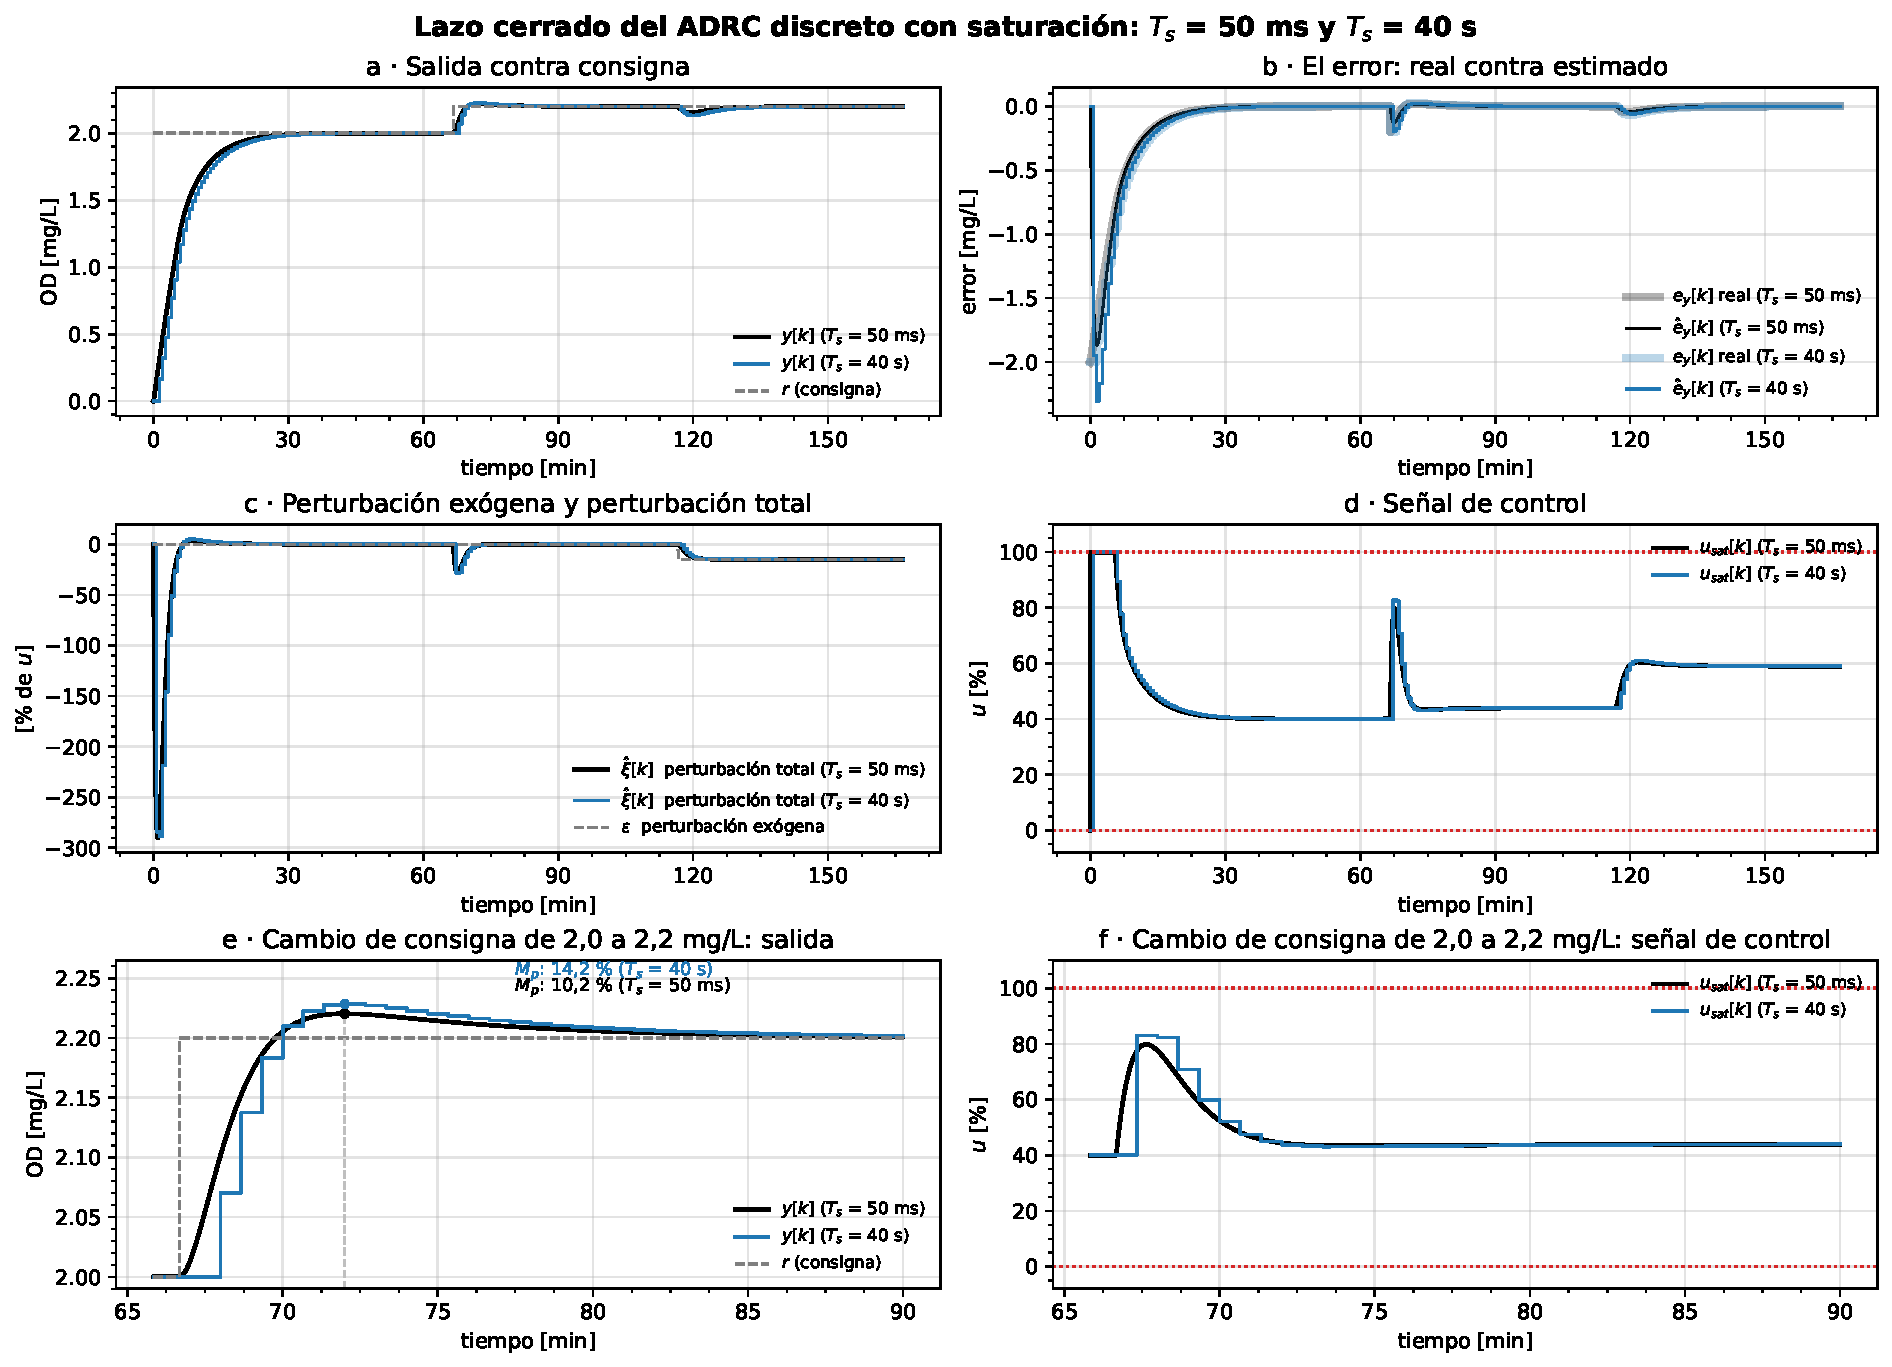
\includegraphics[width=\textwidth]{adrc_discreto_lazo_cerrado.pdf}
  \caption[Lazo cerrado del ADRC discreto con $T_s = 50$~ms y $T_s = 40$~s]{Lazo
    cerrado del ADRC diseñado en discreto, con la planta, el soplador
    limitado entre $0$ y $100~\%$ y el mismo escenario de la
    Figura~\ref{fig:adrc_lazo_cerrado_saturacion}, con $T_s = 50$~ms y
    $T_s = 40$~s, dibujadas en escalones. (a) Salida muestreada $y[k]$ contra
    la consigna. (b) Error de seguimiento real y estimado. (c) Perturbación
    exógena y perturbación total, en \% de $u$. (d) Señal de control.
    (e) y (f) Acercamiento al cambio de consigna de $2{,}0$ a $2{,}2$~mg/L; en (e),
    el sobrepico $M_p$ de cada caso.}
  \label{fig:adrc_discreto_lazo_cerrado}
\end{figure}


\begin{table}[tbp]
\centering
\caption{Matrices del ADRC discreto para el lazo de oxígeno disuelto ($n = 1$,
$m = 1$, $T_s = 50$~ms).}
\label{tab:disc_matrices}
\renewcommand{\arraystretch}{1.6}
\resizebox{\textwidth}{!}{%
\begin{tabular}{lll}
\toprule
\textbf{Sistema} & \textbf{Matrices} & \textbf{Valores} \\
\midrule
Cadena de integradores & $\mathbf{A}_{p,d} = 1,\ \mathbf{B}_{p,d} = T_s$ & $\mathbf{B}_{p,d} = 0{,}05$ \\
Modelo interno & $\mathbf{A}_{\xi,d} = 1,\ \mathbf{B}_{\xi,d} = T_s,\ \mathbf{C}_{\xi} = 1$ & $\mathbf{B}_{\xi,d} = 0{,}05$ \\
Sistema aumentado &
$\mathbf{A}_d = \begin{bmatrix} 1 & T_s \\ 0 & 1 \end{bmatrix},\
\mathbf{B}_d = \begin{bmatrix} T_s \\ 0 \end{bmatrix},\
\mathbf{E}_d = \begin{bmatrix} 0 \\ T_s \end{bmatrix},\
\mathbf{C}_d = \begin{bmatrix} 1 & 0 \end{bmatrix}$ &
$\mathbf{A}_d = \begin{bmatrix} 1 & 0{,}05 \\ 0 & 1 \end{bmatrix},\
\mathbf{B}_d = \begin{bmatrix} 0{,}05 \\ 0 \end{bmatrix},\
\mathbf{E}_d = \begin{bmatrix} 0 \\ 0{,}05 \end{bmatrix}$ \\
Controlabilidad (planta) &
$\mathcal{C}_{p,d} = \mathbf{B}_{p,d} = T_s$ &
$\mathcal{C}_{p,d} = 0{,}05,\ \operatorname{rank}\mathcal{C}_{p,d} = 1$ \\
Observabilidad &
$\mathcal{O}_d = \begin{bmatrix} 1 & 0 \\ 1 & T_s \end{bmatrix},\ \det\mathcal{O}_d = T_s$ &
$\mathcal{O}_d = \begin{bmatrix} 1 & 0 \\ 1 & 0{,}05 \end{bmatrix},\ \operatorname{rank}\mathcal{O}_d = 2$ \\
Polos & $z_c = e^{-\omega_c T_s},\ z_o = e^{-\omega_o T_s}$ & $z_c = 0{,}999833,\ z_o = 0{,}999167$ \\
Controlador &
$\mathbf{K}_d = \begin{bmatrix} (1 - z_c)/T_s & 1 \end{bmatrix}$ &
$\mathbf{K}_d = \begin{bmatrix} 3{,}3331\times10^{-3} & 1 \end{bmatrix}$ \\
Observador &
$\mathbf{L}_d = \begin{bmatrix} 2(1 - z_o) \\ (1 - z_o)^2/T_s \end{bmatrix},\
\mathbf{A}_o = \begin{bmatrix} 1 - l_{1,d} & T_s \\ -l_{2,d} & 1 \end{bmatrix}$ &
$\mathbf{L}_d = \begin{bmatrix} 1{,}6660\times10^{-3} \\ 1{,}3877\times10^{-5} \end{bmatrix},\
\mathbf{A}_o = \begin{bmatrix} 0{,}998334 & 0{,}05 \\ -1{,}3877\times10^{-5} & 1 \end{bmatrix}$ \\
 &
$\mathbf{B}_o = \begin{bmatrix} \mathbf{L}_d & \mathbf{B}_d \end{bmatrix}$ &
$\mathbf{B}_o = \begin{bmatrix} 1{,}6660\times10^{-3} & 0{,}05 \\ 1{,}3877\times10^{-5} & 0 \end{bmatrix}$ \\
Planta &
$\mathbf{A}_{g,d} = e^{-T_s/\tau},\ \mathbf{B}_{g,d} = k_{dc}\,(1 - e^{-T_s/\tau}),\ \mathbf{C}_{g,d} = \mathbf{C}_g = 1$ &
$\mathbf{A}_{g,d} = 0{,}999958,\ \mathbf{B}_{g,d} = 2{,}0833\times10^{-6},\ \mathbf{C}_{g,d} = 1$ \\
\bottomrule
\end{tabular}%
}
\end{table}

\paragraph{Ecuaciones en diferencias.} Para facilitar la implementación en equipos digitales, el
observador se expresa en ecuaciones en diferencias; como el sistema es de orden dos, se tienen dos
ecuaciones en diferencias, una para cada estado estimado. Con
$\widehat{\mathbf{X}}[k] = [\hat{x}_1[k]\ \ \hat{x}_2[k]]^{\top}$, donde
$\hat{x}_1$ estima $e_y$ y $\hat{x}_2$ estima $\xi$, el observador
\eqref{eq:disc_observador} con la orden aplicada es
\begin{equation}
\begin{gathered}
\widehat{\mathbf{X}}[k+1] = \bigl(\mathbf{A}_d - \mathbf{L}_d\,\mathbf{C}_d\bigr)\,\widehat{\mathbf{X}}[k]
+ \mathbf{B}_d\,b_0\,u_{\mathrm{sat}}[k] + \mathbf{L}_d\,e_y[k],
\\[6pt]
\mathbf{A}_d - \mathbf{L}_d\,\mathbf{C}_d =
\begin{bmatrix} a_{11} - l_{1,d}\,c_1 & a_{12} - l_{1,d}\,c_2 \\ a_{21} - l_{2,d}\,c_1 & a_{22} - l_{2,d}\,c_2 \end{bmatrix} .
\end{gathered}
\end{equation}
Fila por fila:
\begin{equation}
\begin{aligned}
\hat{x}_1[k+1] &= (a_{11} - l_{1,d}\,c_1)\,\hat{x}_1[k] + (a_{12} - l_{1,d}\,c_2)\,\hat{x}_2[k] + b_{1,d}\,b_0\,u_{\mathrm{sat}}[k] + l_{1,d}\,e_y[k], \\[2pt]
\hat{x}_2[k+1] &= (a_{21} - l_{2,d}\,c_1)\,\hat{x}_1[k] + (a_{22} - l_{2,d}\,c_2)\,\hat{x}_2[k] + b_{2,d}\,b_0\,u_{\mathrm{sat}}[k] + l_{2,d}\,e_y[k] .
\end{aligned}
\end{equation}
Con $a_{11} = 1$, $a_{12} = T_s$, $a_{21} = 0$, $a_{22} = 1$, $b_{1,d} = T_s$,
$b_{2,d} = 0$, $c_1 = 1$ y $c_2 = 0$ (Tabla~\ref{tab:disc_matrices}):
\begin{equation}
\begin{aligned}
\hat{x}_1[k+1] &= (1 - l_{1,d})\,\hat{x}_1[k] + T_s\,\hat{x}_2[k] + T_s\,b_0\,u_{\mathrm{sat}}[k] + l_{1,d}\,e_y[k], \\[2pt]
\hat{x}_2[k+1] &= -\,l_{2,d}\,\hat{x}_1[k] + \hat{x}_2[k] + l_{2,d}\,e_y[k] .
\end{aligned}
\label{eq:disc_filas}
\end{equation}
Para implementarlo se escribe con retardos, desplazando un periodo
($k \to k-1$):
\begin{equation}
\begin{aligned}
\hat{x}_1[k] &= (1 - l_{1,d})\,\hat{x}_1[k-1] + T_s\,\hat{x}_2[k-1] + T_s\,b_0\,u_{\mathrm{sat}}[k-1] + l_{1,d}\,e_y[k-1], \\[2pt]
\hat{x}_2[k] &= -\,l_{2,d}\,\hat{x}_1[k-1] + \hat{x}_2[k-1] + l_{2,d}\,e_y[k-1] .
\end{aligned}
\label{eq:disc_filas_retardos}
\end{equation}
Las dos ecuaciones usan solo valores del periodo anterior; en el PLC se
calculan con copias de $\hat{x}_1[k-1]$ y $\hat{x}_2[k-1]$, es decir, con la información de cada
variable guardada previamente en memoria, para que
$\hat{x}_2[k]$ no use el $\hat{x}_1[k]$ ya actualizado.
La ley de control \eqref{eq:disc_ley}, con $\mathbf{K}_d = [k_{p,d}\ \ \mathbf{C}_{\xi,d}] = [k_{p,d}\ \ 1]$, es
\begin{equation}
u_0[k] = -\bigl(k_{p,d}\,\hat{x}_1[k] + \hat{x}_2[k]\bigr),
\qquad
u[k] = \frac{u_0[k]}{b_0},
\qquad
u_{\mathrm{sat}}[k] = \operatorname{sat}_{0}^{100}\bigl(u[k]\bigr) .
\label{eq:disc_ley_escalar}
\end{equation}
$u_0$ es la orden normalizada que actúa sobre la cadena de integradores; $b_0$
solo convierte entre $u_0$ y la orden del soplador, a la salida
($u = u_0/b_0$) y en la realimentación al observador ($b_0\,u_{\mathrm{sat}}$).
Con $T_s = 50$~ms, $k_{p,d}$, $l_{1,d}/T_s$ y $l_{2,d}/T_s$ difieren de
$\omega_c$, $2\omega_o$ y $\omega_o^2$ en menos de $0{,}1~\%$
(Tabla~\ref{tab:disc_matrices}).
\paragraph{Realización con retardos.} Las ecuaciones \eqref{eq:disc_filas_retardos}
y \eqref{eq:disc_ley_escalar} se realizan con dos retardos, uno por estado del
observador (Figura~\ref{fig:adrc_discreto_retardos}); es decir, son necesarios dos retardos y
tres bloques de suma para implementarlo en cualquier equipo digital.

\begin{figure}[H]
  \centering
  \resizebox{\textwidth}{!}{%
  \begin{tikzpicture}[every path/.style={thick}, >={Stealth},
        g/.style={draw, thick, minimum width=1.25cm, minimum height=0.65cm, inner sep=2pt},
        dl/.style={draw, thick, minimum width=1.0cm, minimum height=0.7cm},
        blk/.style={draw, thick, minimum size=0.8cm}]
    % ganancias del observador
    \node[g] (g1a) at (3.9, 1.5) {$l_{1,d}$};
    \node[g] (g1b) at (3.9, 0.5) {$T_s\,b_0$};
    \node[g] (g1c) at (3.9,-0.5) {$1 - l_{1,d}$};
    \node[g] (g1d) at (3.9,-1.5) {$T_s$};
    \node[g] (g2a) at (3.9,-3.5) {$l_{2,d}$};
    \node[g] (g2b) at (3.9,-4.5) {$-l_{2,d}$};
    \node[g] (g2c) at (3.9,-5.5) {$1$};
    \node[sum, minimum size=0.5cm] (S1) at (5.9, 0)   {$+$};
    \node[sum, minimum size=0.5cm] (S2) at (5.9,-4.5) {$+$};
    \node[dl] (D1) at (8.3, 0)   {$z^{-1}$};
    \node[dl] (D2) at (8.3,-4.5) {$z^{-1}$};
    \foreach \n in {g1a,g1b,g1c,g1d} \draw[->] (\n.east) -- (S1);
    \foreach \n in {g2a,g2b,g2c} \draw[->] (\n.east) -- (S2);
    \draw[->] (S1.east) -- node[above] {$\hat{x}_1[k+1]$} (D1.west);
    \draw[->] (S2.east) -- node[above] {$\hat{x}_2[k+1]$} (D2.west);
    \draw (D1.east) -- (9.9,0);
    \draw (D2.east) -- (9.9,-4.5);
    \fill (9.9,0) circle (1.5pt);
    \fill (9.9,-4.5) circle (1.5pt);
    \node[above right] at (8.85,0) {$\hat{x}_1[k]$};
    \node[above right] at (8.85,-4.5) {$\hat{x}_2[k]$};

    % entrada e_y[k]
    \draw (-0.8,1.5) node[left] {$e_y[k]$} -- (0.8,1.5);
    \fill (0.8,1.5) circle (1.5pt);
    \draw[->] (0.8,1.5) -- (g1a.west);
    \draw (0.8,1.5) -- (0.8,-3.5);
    \draw[->] (0.8,-3.5) -- (g2a.west);

    % realimentacion de x1 (por arriba) y de x2 (por abajo)
    \draw (9.9,0) -- (9.9,2.6) -- (2.0,2.6) -- (2.0,-4.5);
    \fill (2.0,-0.5) circle (1.5pt);
    \draw[->] (2.0,-0.5) -- (g1c.west);
    \draw[->] (2.0,-4.5) -- (g2b.west);
    \draw (9.9,-4.5) -- (9.9,-6.6) -- (2.6,-6.6) -- (2.6,-1.5);
    \fill (2.6,-5.5) circle (1.5pt);
    \draw[->] (2.6,-5.5) -- (g2c.west);
    \draw[->] (2.6,-1.5) -- (g1d.west);

    % ley de control
    \node[g] (kp) at (11.5, 0)   {$-k_{p,d}$};
    \node[g] (k1) at (11.5,-4.5) {$-1$};
    \node[sum, minimum size=0.5cm] (S3) at (13.2,-2.25) {$+$};
    \node[blk] (ib) at (14.7,-2.25) {$1/b_0$};
    \draw[->] (9.9,0) -- (kp.west);
    \draw[->] (9.9,-4.5) -- (k1.west);
    \draw[->] (kp.east) -- (S3);
    \draw[->] (k1.east) -- (S3);
    \draw[->] (S3.east) -- node[above] {$u_0[k]$} (ib.west);
    \draw[->] (ib.east) -- (16.8,-2.25) node[right] {$u[k]$};

    % orden aplicada al observador
    \draw[->] (-0.8,0.5) node[left] {$u_{\mathrm{sat}}[k]$} -- (g1b.west);
  \end{tikzpicture}%
  }
  \caption[Realización con retardos del ADRC discreto]{Realización con
    retardos del ADRC discreto: observador \eqref{eq:disc_filas_retardos} y ley
    de control \eqref{eq:disc_ley_escalar}. A la entrada de cada $z^{-1}$ está
    $\hat{x}_i[k+1]$ y a la salida $\hat{x}_i[k]$; la orden aplicada
    $u_{\mathrm{sat}}[k]$ entra al observador con la ganancia $T_s\,b_0$.}
  \label{fig:adrc_discreto_retardos}
\end{figure}

%--------------------------------------------------------------------
\subsection{GPI robusto discreto}
\label{subsec:disc_gpi}

Cada función de transferencia del lazo de las
Figuras~\ref{fig:gpi_antiwindup_ganancias} y~\ref{fig:gpi_antiwindup_wo} se discretiza con
Tustin \eqref{eq:disc_metodos}, el método que más se parece al continuo en la
Figura~\ref{fig:disc_metodos_bode_40}: $H_1 = P/E_1$ (entra $-e_y$, sale $v_1$),
$H_2 = (L - E_1)/E_1$ (entra $u_{\mathrm{sat}}$, sale $v_2$) y la planta $G$ (entra
$\bar{u}$, sale $y$); $1/b_0$ es una ganancia estática y no cambia. Con los dos $E_1$,
\eqref{eq:aw_gpi} y \eqref{eq:aw_gpi_wo}, $H_1$ y $H_2$ son de grado $2$ sobre grado $2$ con el
mismo denominador, así que con $s \to \frac{2}{T_s}\,\frac{1 - z^{-1}}{1 + z^{-1}}$ quedan con
la misma forma:
\begin{equation}
\begin{aligned}
H_1(s) &= \frac{P(s)}{E_1(s)} & \;\longrightarrow\; H_1(z) &= \frac{\beta_0 + \beta_1 z^{-1} + \beta_2 z^{-2}}{1 + \alpha_1 z^{-1} + \alpha_2 z^{-2}}, \\[6pt]
H_2(s) &= \frac{L(s) - E_1(s)}{E_1(s)} & \;\longrightarrow\; H_2(z) &= \frac{\bar{\gamma}_0 + \bar{\gamma}_1 z^{-1} + \bar{\gamma}_2 z^{-2}}{1 + \alpha_1 z^{-1} + \alpha_2 z^{-2}}, \\[6pt]
G(s) &= \frac{k_{dc}}{\tau s + 1} & \;\longrightarrow\; G(z) &= \frac{\beta_g\,\bigl(1 + z^{-1}\bigr)}{1 + \alpha_g z^{-1}} .
\end{aligned}
\label{eq:disc_gpi_tf}
\end{equation}
Solo cambian los valores de los coeficientes, dependiendo de si se usa $E_1 = s^2 + k_2 s + k_1$
o $E_1 = (s + \omega_o)^2$ (Tabla~\ref{tab:disc_gpi_coef}).


\begin{table}[H]
\centering
\caption[Coeficientes del GPI y de la planta discretizados con Tustin]{Coeficientes
  de \eqref{eq:disc_gpi_tf} con los dos $E_1$, con $k_0$, $k_1$ y $k_2$ de la
  Sección~\ref{sec:gpi_caso} y $b_0 = 4{,}1667\times10^{-5}$.}
\label{tab:disc_gpi_coef}
\renewcommand{\arraystretch}{1.3}
\small
\begin{tabular}{llll}
\toprule
 & \textbf{Expresión} & $\boldsymbol{T_s = 50}$~\textbf{ms} & $\boldsymbol{T_s = 40}$~\textbf{s} \\
\midrule
\multicolumn{4}{l}{\textbf{Con las ganancias}, $E_1 = s^2 + k_2 s + k_1$ \eqref{eq:aw_gpi}} \\
$D_0$      & $4 + 2k_2 T_s + k_1 T_s^2$                    & $4{,}0036676$              & $7{,}5555556$ \\
$\alpha_1$ & $(2k_1 T_s^2 - 8)/D_0$                        & $-1{,}99816737$            & $-0{,}89411765$ \\
$\alpha_2$ & $(4 - 2k_2 T_s + k_1 T_s^2)/D_0$              & $0{,}99816835$             & $0{,}22352941$ \\
$\beta_0$  & $(k_0 T_s^2 + 2k_1 T_s)/D_0$                  & $9{,}71389\times10^{-6}$   & $4{,}31373\times10^{-3}$ \\
$\beta_1$  & $2k_0 T_s^2/D_0$                              & $1{,}15635\times10^{-9}$   & $3{,}92157\times10^{-4}$ \\
$\beta_2$  & $(k_0 T_s^2 - 2k_1 T_s)/D_0$                  & $-9{,}71274\times10^{-6}$  & $-3{,}92157\times10^{-3}$ \\
$\bar{\gamma}_0$ & $-k_1 T_s^2/D_0 = -\rho$                      & $-2{,}42833\times10^{-7}$  & $-8{,}23529\times10^{-2}$ \\
$\bar{\gamma}_1$ & $-2k_1 T_s^2/D_0 = -2\rho$                    & $-4{,}85666\times10^{-7}$  & $-1{,}64706\times10^{-1}$ \\
$\bar{\gamma}_2$ & $-k_1 T_s^2/D_0 = -\rho$                      & $-2{,}42833\times10^{-7}$  & $-8{,}23529\times10^{-2}$ \\
\midrule
\multicolumn{4}{l}{\textbf{Con el observador}, $E_1 = (s + \omega_o)^2$ \eqref{eq:aw_gpi_wo}} \\
$D_0$      & $(2 + \omega_o T_s)^2$                                         & $4{,}0033340$              & $7{,}1111111$ \\
$\alpha_1$ & $-2\,(4 - \omega_o^2 T_s^2)/D_0$                               & $-1{,}99833403$            & $-1$ \\
$\alpha_2$ & $(2 - \omega_o T_s)^2/D_0$                                     & $0{,}99833472$             & $0{,}25$ \\
$\beta_0$  & $\omega_o T_s\,[\omega_c\omega_o T_s + 2(\omega_o + 2\omega_c)]/D_0$ & $9{,}71470\times10^{-6}$ & $4{,}58333\times10^{-3}$ \\
$\beta_1$  & $2\,\omega_c\omega_o^2 T_s^2/D_0$                              & $1{,}15644\times10^{-9}$   & $4{,}16667\times10^{-4}$ \\
$\beta_2$  & $\omega_o T_s\,[\omega_c\omega_o T_s - 2(\omega_o + 2\omega_c)]/D_0$ & $-9{,}71355\times10^{-6}$ & $-4{,}16667\times10^{-3}$ \\
$\bar{\gamma}_0$ & $T_s\,(2\omega_c - \omega_o^2 T_s)/D_0$                        & $8{,}30905\times10^{-5}$   & $-0{,}025$ \\
$\bar{\gamma}_1$ & $-2\,\omega_o^2 T_s^2/D_0$                                     & $-3{,}46933\times10^{-7}$  & $-0{,}125$ \\
$\bar{\gamma}_2$ & $-T_s\,(2\omega_c + \omega_o^2 T_s)/D_0$                       & $-8{,}34374\times10^{-5}$  & $-0{,}1$ \\
\midrule
\multicolumn{4}{l}{\textbf{Planta}} \\
$\beta_g$  & $k_{dc}\,T_s/(2\tau + T_s)$                   & $1{,}04164\times10^{-6}$   & $8{,}19672\times10^{-4}$ \\
$\alpha_g$ & $(T_s - 2\tau)/(2\tau + T_s)$                 & $-0{,}99995833$            & $-0{,}96721311$ \\
\bottomrule
\end{tabular}
\end{table}


Ahora bien, la Figura~\ref{fig:gpi_discreto} muestra cómo queda el lazo cerrado en discreto con los
bloques $H_1$ y $H_2$ y sus respectivos coeficientes. Hay que recordar que, cuando el sistema no se
satura, $u = v$ y la dinámica vuelve a ser la diseñada.


\begin{figure}[H]
  \centering
  \resizebox{\textwidth}{!}{%
  \begin{tikzpicture}[every path/.style={thick}]
    \node[sum] (s1) at (1.0,0) {};
    \node[block, minimum width=4.2cm, minimum height=1.3cm] (pe) at (5.0,0)
      {$\dfrac{\beta_0 + \beta_1 z^{-1} + \beta_2 z^{-2}}{1 + \alpha_1 z^{-1} + \alpha_2 z^{-2}}$};
    \node[above=1pt of pe] {$H_1(z)$};
    \node[block, minimum size=9mm] (ib) at (8.8,0) {$1/b_0$};
    \node[sum] (s2) at (10.2,0) {};

    % saturacion (icono clasico de Simulink)
    \node[block, minimum size=11mm] (sat) at (12.2,0) {};
    \draw[thin, gray] ($(sat.center)+(-0.38,0)$) -- ($(sat.center)+(0.38,0)$);
    \draw[thin, gray] ($(sat.center)+(0,-0.38)$) -- ($(sat.center)+(0,0.38)$);
    \draw[line width=1.1pt] ($(sat.center)+(-0.38,-0.22)$) -- ($(sat.center)+(-0.18,-0.22)$)
                         -- ($(sat.center)+(0.18,0.22)$) -- ($(sat.center)+(0.38,0.22)$);
    \node[above=1pt of sat, font=\small] {0--100~\%};

    \coordinate (us) at (14.8,0);
    \node[block, minimum width=4.2cm, minimum height=1.3cm] (fb) at (12.5,-2.1)
      {$\dfrac{\bar{\gamma}_0 + \bar{\gamma}_1 z^{-1} + \bar{\gamma}_2 z^{-2}}{1 + \alpha_1 z^{-1} + \alpha_2 z^{-2}}$};
    \node[below=1pt of fb] {$H_2(z)$};
    \node[sum] (s3) at (16.3,0) {};
    \node[block, minimum width=1.6cm, minimum height=1.1cm] (plant) at (18.6,0) {$G(z)$};
    \coordinate (yb) at (20.1,0);

    % --- recuadro del controlador ---
    \draw[red, dashed, thick] (2.5,1.75) rectangle (15.2,-3.35);
    \node[below left] at (15.2,1.75) {GPI discreto};

    % --- señales ---
    \draw[->] (-0.9,0) node[above right] {$r[k]$} -- (s1.west);
    \node[sgn] at ($(s1.west)+(-0.15,0.25)$) {$+$};
    \draw[->] (s1.east) -- node[above, pos=0.4] {$-e_y[k]$} (pe.west);
    \draw[->] (pe.east) -- node[above] {$v_1[k]$} (ib.west);
    \draw[->] (ib.east) -- (s2.west);
    \node[sgn] at ($(s2.west)+(-0.2,0.25)$) {$+$};
    \draw[->] (s2.east) -- node[above] {$v[k]$} (sat.west);
    \draw (sat.east) -- node[above] {$u_{\mathrm{sat}}[k]$} (us);
    \fill (us) circle (1.5pt);
    \draw[->] (us) -- (s3.west);
    \node[sgn] at ($(s3.west)+(-0.2,-0.25)$) {$+$};
    \draw[->] (s3 |- 0,1.6) node[above] {$\varepsilon[k]$} -- (s3.north);
    \node[sgn] at ($(s3.north)+(-0.25,0.2)$) {$+$};
    \draw[->] (s3.east) -- node[above] {$\bar{u}[k]$} (plant.west);
    \draw[->] (us) -- (us |- fb) -- (fb.east);
    \draw[->] (fb.west) -- (s2 |- fb) -- node[left, pos=0.5] {$v_2[k]$} (s2.south);
    \node[sgn] at ($(s2.south)+(0.25,-0.2)$) {$-$};
    \draw (plant.east) -- (yb);
    \draw[->] (yb) -- (21.2,0) node[above left] {$y[k]$};
    \fill (yb) circle (1.5pt);
    \draw[->] (yb) -- (20.1,-3.9) -- (1.0,-3.9) -- (s1.south);
    \node[sgn] at ($(s1.south)+(-0.25,-0.15)$) {$-$};
  \end{tikzpicture}%
  }
  \caption[GPI discreto con realimentación de la saturación]{GPI discreto con
    realimentación de la saturación: cada bloque de las
    Figuras~\ref{fig:gpi_antiwindup_ganancias} y~\ref{fig:gpi_antiwindup_wo} y la planta
    discretizados con Tustin \eqref{eq:disc_gpi_tf}. La estructura es la misma con los dos
    $E_1$; solo cambian los coeficientes (Tabla~\ref{tab:disc_gpi_coef}).}
  \label{fig:gpi_discreto}
\end{figure}
\paragraph{Simulación.} En el cambio de consigna de $2{,}0$ a $2{,}2$~mg/L el
soplador no se satura, así que $u = v$ y, con cualquiera de los dos $E_1$, el controlador es
$C(z) = \frac{1}{b_0}\,H_1(z)/\bigl(1 + H_2(z)\bigr)$, exactamente el Tustin de
$C(s)$. La Figura~\ref{fig:gpi_discreto_vs_adrc} compara ese lazo, con la
planta también por Tustin, con el ADRC discreto de la
Figura~\ref{fig:adrc_discreto_lazo_cerrado}. Con $T_s = 50$~ms coinciden; con
$T_s = 40$~s el GPI responde desde la misma muestra del cambio, porque Tustin, en su realización,
deja términos directos en el controlador ($\beta_0$) y en la planta ($\beta_g$), mientras que el
ADRC usa el error del periodo anterior. Esto quiere decir que Tustin tiende a estar más en fase y no
se atrasa tanto como otras discretizaciones.

\begin{figure}[H]
  \centering
  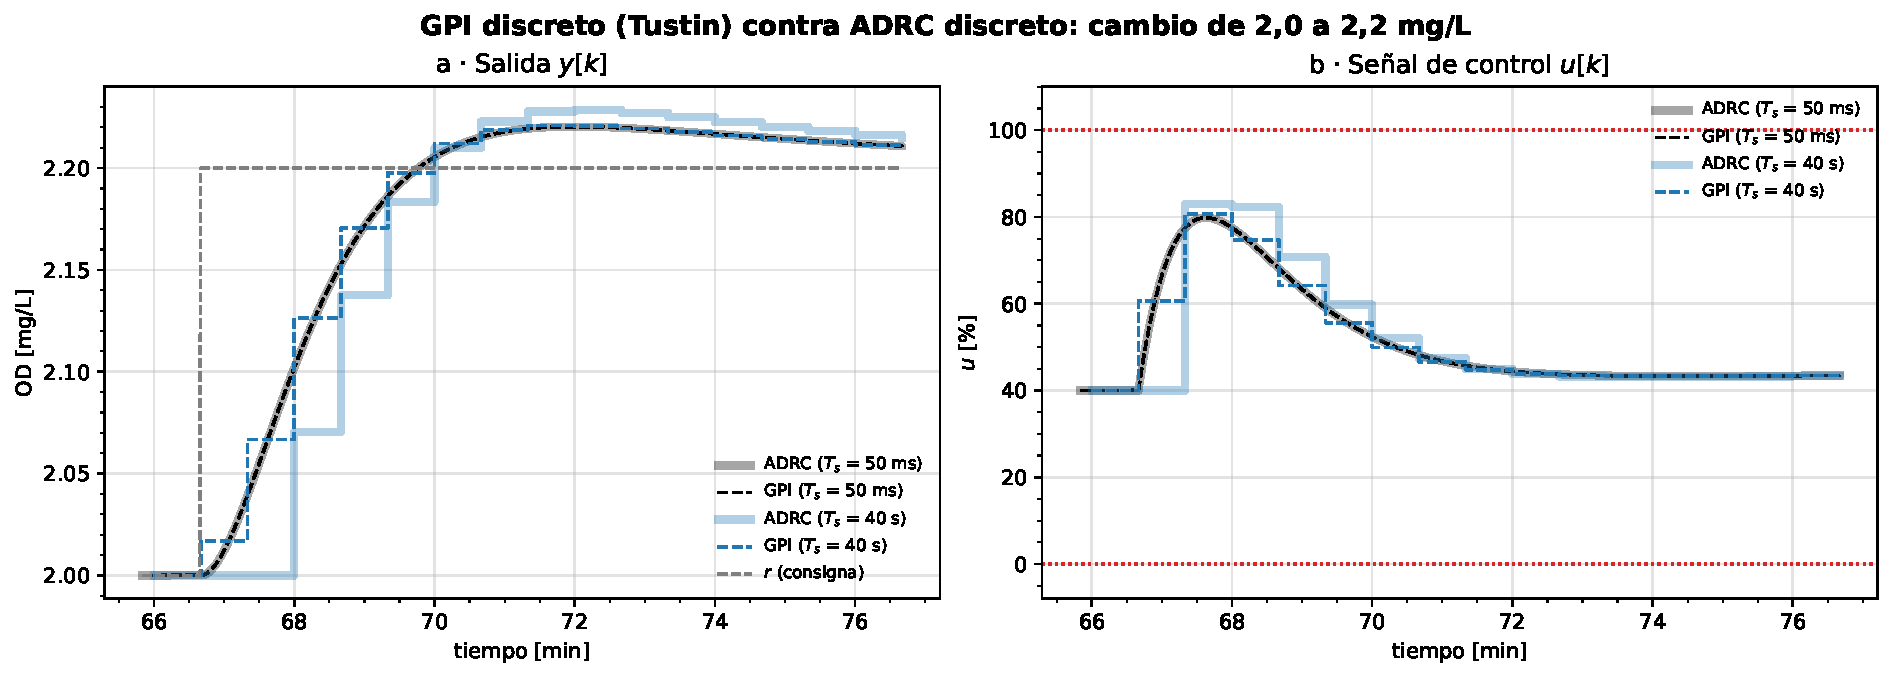
\includegraphics[width=\textwidth]{gpi_discreto_vs_adrc.pdf}
  \caption[GPI discreto contra ADRC discreto]{GPI discreto con
    $E_1 = (s + \omega_o)^2$ \eqref{eq:aw_gpi_wo}, con controlador y
    planta por Tustin (discontinua), contra ADRC discreto con la planta exacta
    (banda), en el cambio de consigna de $2{,}0$ a $2{,}2$~mg/L, sin
    saturación, con $T_s = 50$~ms (negro) y $T_s = 40$~s (azul), dibujados en
    escalones. (a) Salida $y[k]$. (b) Señal de control $u[k]$.}
  \label{fig:gpi_discreto_vs_adrc}
\end{figure}

\paragraph{Ecuaciones en diferencias.} Para facilitar la implementación, las funciones de
transferencia en $z$ se pasan a ecuaciones en diferencias en el tiempo discreto, con $x[k] = -e_y[k]$:
\begin{equation}
\begin{aligned}
v_1[k] &= \beta_0\,x[k] + \beta_1\,x[k-1] + \beta_2\,x[k-2] - \alpha_1\,v_1[k-1] - \alpha_2\,v_1[k-2], \\[2pt]
v_2[k] &= \bar{\gamma}_0\,u_{\mathrm{sat}}[k] + \bar{\gamma}_1\,u_{\mathrm{sat}}[k-1] + \bar{\gamma}_2\,u_{\mathrm{sat}}[k-2] - \alpha_1\,v_2[k-1] - \alpha_2\,v_2[k-2], \\[2pt]
v[k] &= \frac{v_1[k]}{b_0} - v_2[k], \qquad u_{\mathrm{sat}}[k] = \operatorname{sat}_{0}^{100}\bigl(v[k]\bigr) .
\end{aligned}
\label{eq:disc_gpi_dif}
\end{equation}
\paragraph{Realización.} Como $H_1$ y $H_2$ comparten el denominador, los dos
bloques se realizan juntos en forma directa I \cite{chen1993analog}, con
entradas $-e_y[k]$ y $u_{\mathrm{sat}}[k]$ y salida $v[k]$
(Figura~\ref{fig:disc_formas_directas}). De
$v = H_1\,(-e_y)/b_0 - H_2\,u_{\mathrm{sat}}$, la función de transferencia
discreta completa del controlador tiene dos entradas y una salida, y se puede escribir en la
siguiente forma compacta:
\begin{equation}
V(z) =
\begin{bmatrix}
\dfrac{\beta_0 + \beta_1 z^{-1} + \beta_2 z^{-2}}{b_0\,\bigl(1 + \alpha_1 z^{-1} + \alpha_2 z^{-2}\bigr)}
&
\dfrac{-\bigl(\bar{\gamma}_0 + \bar{\gamma}_1 z^{-1} + \bar{\gamma}_2 z^{-2}\bigr)}{1 + \alpha_1 z^{-1} + \alpha_2 z^{-2}}
\end{bmatrix}
\begin{bmatrix} -E_y(z) \\[4pt] U_{\mathrm{sat}}(z) \end{bmatrix},
\label{eq:disc_gpi_miso}
\end{equation}
y en forma directa I, con $x[k] = -e_y[k]$:
\begin{equation}
\begin{aligned}
v[k] = {} & \frac{\beta_0\,x[k] + \beta_1\,x[k-1] + \beta_2\,x[k-2]}{b_0}
- \bigl(\bar{\gamma}_0\,u_{\mathrm{sat}}[k] + \bar{\gamma}_1\,u_{\mathrm{sat}}[k-1] + \bar{\gamma}_2\,u_{\mathrm{sat}}[k-2]\bigr) \\
& - \alpha_1\,v[k-1] - \alpha_2\,v[k-2] .
\end{aligned}
\label{eq:disc_gpi_fd1}
\end{equation}
Son seis retardos y un solo sumador. Los estados son señales del lazo, con
rangos conocidos, y se pueden inicializar al arrancar. Hay que trabajar en doble precisión (LREAL en el PLC, de 64 bits, y no REAL de 32 bits): con $T_s = 50$~ms los polos de
$E_1(z)$ están en $|z| = 0{,}99908$ con las ganancias y en $0{,}99917$ (doble) con el
observador, y $1 + \alpha_1 + \alpha_2$ vale $9{,}7\times10^{-7}$ y $6{,}9\times10^{-7}$; por
eso $\alpha_1$ y $\alpha_2$ llevan ocho decimales, y para evitar problemas posteriores de precisión es mejor usar LREAL. 

\begin{figure}[H]
  \centering
  \resizebox{0.75\textwidth}{!}{%
  \begin{tikzpicture}[every path/.style={thick},
      g/.style={draw, thick, minimum width=0.9cm, minimum height=0.7cm, inner sep=2pt},
      dl/.style={draw, thick, minimum width=0.95cm, minimum height=0.6cm}]
    % --- entrada -e_y ---
    \node[g] (a0) at (2.9,0)    {$\beta_0/b_0$};
    \node[g] (a1) at (2.9,-1.6) {$\beta_1/b_0$};
    \node[g] (a2) at (2.9,-3.2) {$\beta_2/b_0$};
    \node[dl] (dx1) at (0.9,-0.8) {$z^{-1}$};
    \node[dl] (dx2) at (0.9,-2.4) {$z^{-1}$};
    % --- entrada u_sat ---
    \node[g] (c0) at (2.9,-4.8) {$-\bar{\gamma}_0$};
    \node[g] (c1) at (2.9,-6.4) {$-\bar{\gamma}_1$};
    \node[g] (c2) at (2.9,-8.0) {$-\bar{\gamma}_2$};
    \node[dl] (du1) at (0.9,-5.6) {$z^{-1}$};
    \node[dl] (du2) at (0.9,-7.2) {$z^{-1}$};
    % --- sumador y salida ---
    \node[sum, minimum size=0.55cm] (S) at (5.2,-4.0) {$+$};
    \node[g] (e1) at (6.4,-5.6) {$-\alpha_1$};
    \node[g] (e2) at (6.4,-7.2) {$-\alpha_2$};
    \node[dl] (dv1) at (7.8,-4.8) {$z^{-1}$};
    \node[dl] (dv2) at (7.8,-6.4) {$z^{-1}$};

    \draw[->] (-0.6,0) node[left] {$-e_y[k]$} -- (a0.west);
    \fill (0.9,0) circle (1.5pt);
    \draw[->] (0.9,0) -- (dx1.north);
    \draw (dx1.south) -- (0.9,-1.6);
    \fill (0.9,-1.6) circle (1.5pt);
    \draw[->] (0.9,-1.6) -- (a1.west);
    \draw[->] (0.9,-1.6) -- (dx2.north);
    \draw (dx2.south) -- (0.9,-3.2);
    \draw[->] (0.9,-3.2) -- (a2.west);
    \node[font=\scriptsize, left] at (0.9,-1.6) {$-e_y[k-1]$};
    \node[font=\scriptsize, left] at (0.9,-3.2) {$-e_y[k-2]$};

    \draw[->] (-0.6,-4.8) node[left] {$u_{\mathrm{sat}}[k]$} -- (c0.west);
    \fill (0.9,-4.8) circle (1.5pt);
    \draw[->] (0.9,-4.8) -- (du1.north);
    \draw (du1.south) -- (0.9,-6.4);
    \fill (0.9,-6.4) circle (1.5pt);
    \draw[->] (0.9,-6.4) -- (c1.west);
    \draw[->] (0.9,-6.4) -- (du2.north);
    \draw (du2.south) -- (0.9,-8.0);
    \draw[->] (0.9,-8.0) -- (c2.west);
    \node[font=\scriptsize, left] at (0.9,-6.4) {$u_{\mathrm{sat}}[k-1]$};
    \node[font=\scriptsize, left] at (0.9,-8.0) {$u_{\mathrm{sat}}[k-2]$};

    \foreach \n in {a0,a1,a2,c0,c1,c2} \draw[->] (\n.east) -- (S);
    \draw[->] (e1.north west) -- (S);
    \draw[->] (e2.north west) -- (S);

    \draw[->] (S.east) -- (9.0,-4.0) node[right] {$v[k]$};
    \fill (7.8,-4.0) circle (1.5pt);
    \draw[->] (7.8,-4.0) -- (dv1.north);
    \draw (dv1.south) -- (7.8,-5.6);
    \fill (7.8,-5.6) circle (1.5pt);
    \draw[->] (7.8,-5.6) -- (e1.east);
    \draw[->] (7.8,-5.6) -- (dv2.north);
    \draw (dv2.south) -- (7.8,-7.2);
    \draw[->] (7.8,-7.2) -- (e2.east);
    \node[font=\scriptsize, right] at (7.8,-5.6) {$v[k-1]$};
    \node[font=\scriptsize, right] at (7.8,-7.2) {$v[k-2]$};
  \end{tikzpicture}%
  }
  \caption[Realización en forma directa I del GPI discreto]{Realización en
    forma directa I de los dos bloques del GPI discreto juntos
    \eqref{eq:disc_gpi_fd1}: entradas $-e_y[k]$ y $u_{\mathrm{sat}}[k]$,
    salida $v[k]$. Es la misma estructura con los dos $E_1$; solo cambian los
    coeficientes de la Tabla~\ref{tab:disc_gpi_coef}.}
  \label{fig:disc_formas_directas}
\end{figure}


%--------------------------------------------------------------------
\subsection{Prefiltro de consigna discreto}
\label{subsec:disc_prefiltro}

El prefiltro \eqref{eq:pref_f} se discretiza con Tustin \eqref{eq:disc_metodos}, igual que el GPI.
Con $s \to \frac{2}{T_s}\,\frac{1 - z^{-1}}{1 + z^{-1}}$,
\begin{equation}
F(s) = \frac{k_0}{k_1 s + k_0}
\quad\longrightarrow\quad
F(z) = \frac{\beta_f\,\bigl(1 + z^{-1}\bigr)}{1 + \alpha_f\,z^{-1}},
\qquad
\alpha_f = \frac{k_0 T_s - 2 k_1}{k_0 T_s + 2 k_1},
\qquad
\beta_f = \frac{k_0 T_s}{k_0 T_s + 2 k_1} .
\label{eq:disc_pref_tf}
\end{equation}
Las dos son ganancias fijas: se calculan una vez y solo cambian con $k_0$, $k_1$ o $T_s$; $k_2$ no
entra. En términos de los anchos de banda,
\begin{equation}
\alpha_f = \frac{\omega_c\,\omega_o\,T_s - 2\,(\omega_o + 2\,\omega_c)}{\omega_c\,\omega_o\,T_s + 2\,(\omega_o + 2\,\omega_c)},
\qquad
\beta_f = \frac{\omega_c\,\omega_o\,T_s}{\omega_c\,\omega_o\,T_s + 2\,(\omega_o + 2\,\omega_c)} .
\end{equation}
La ganancia estática es exactamente $F(1) = 2\beta_f/(1 + \alpha_f) = 1$. Como Tustin es una
sustitución de $s$, el polo de $F(z)$ es la imagen del cero del lazo y la cancelación de
\eqref{eq:pref_yr_f} se conserva exacta con el GPI discreto. La Tabla~\ref{tab:disc_pref} resume los
valores.

\begin{table}[H]
\centering
\caption{Ganancias del prefiltro discreto \eqref{eq:disc_pref_tf}.}
\label{tab:disc_pref}
\renewcommand{\arraystretch}{1.3}
\begin{tabular}{llll}
\toprule
 & \textbf{Expresión} & $\boldsymbol{T_s = 50}$~\textbf{ms} & $\boldsymbol{T_s = 40}$~\textbf{s} \\
\midrule
$\alpha_f$ & $(k_0 T_s - 2 k_1)/(k_0 T_s + 2 k_1)$ & $-0{,}99988096$ & $-0{,}90909091$ \\
$\beta_f$ & $k_0 T_s/(k_0 T_s + 2 k_1)$ & $5{,}952027\times10^{-5}$ & $4{,}545455\times10^{-2}$ \\
\bottomrule
\end{tabular}
\end{table}

\paragraph{Ecuación en diferencias.} Para simplificar la implementación, el prefiltro se presenta
como una ecuación en diferencias:
\begin{equation}
r_f[k] = -\alpha_f\,r_f[k-1] + \beta_f\,\bigl(r[k] + r[k-1]\bigr),
\qquad
e_y[k] = y[k] - r_f[k] .
\label{eq:disc_pref_dif}
\end{equation}
Con $T_s = 50$~ms, $\beta_f$ es del orden de $10^{-5}$, así que hay que trabajar en doble precisión
(LREAL), como en el GPI.

La Figura~\ref{fig:disc_prefiltro_retardo} muestra el cambio de consigna con el prefiltro discreto, con
la planta exacta y con $\theta = 0$ y $50$~s, y la Tabla~\ref{tab:disc_prefiltro_indices} resume sus
índices. En ningún caso hay sobrepico. Con $T_s = 50$~ms, el ADRC con ESO y el GPI discretos se comportan
igual: tienen el mismo tiempo de asentamiento y el mismo pico de la señal de control, y el retardo
solo alarga un poco el transitorio y sube el pico de $u$. Cuando se aumenta el tiempo de muestreo a
$T_s = 40$~s ya se ven diferencias: el ADRC  con ESO se asienta un poco antes, el pico de $u$ sube, sobre todo
con el GPI, y con $\theta = 50$~s aparece una pequeña oscilación en la señal de control. Aun así, en
todos los casos el prefiltro discreto funciona adecuadamente: la salida llega a la consigna sin
sobrepico y la señal de control queda lejos de la saturación. Además, el $t_s$ coincide con el que se
buscó al elegir $\omega_c = 4/\tau$: con $\tau = 20$~min en la planta y el controlador acelerándola a
cuatro veces la velocidad del lazo abierto, el sistema debería estabilizarse cerca de los $20$~min en
lazo cerrado, según el criterio que se use, lo cual es adecuado y se comprueba con este experimento.

\begin{figure}[tbp]
  \centering
  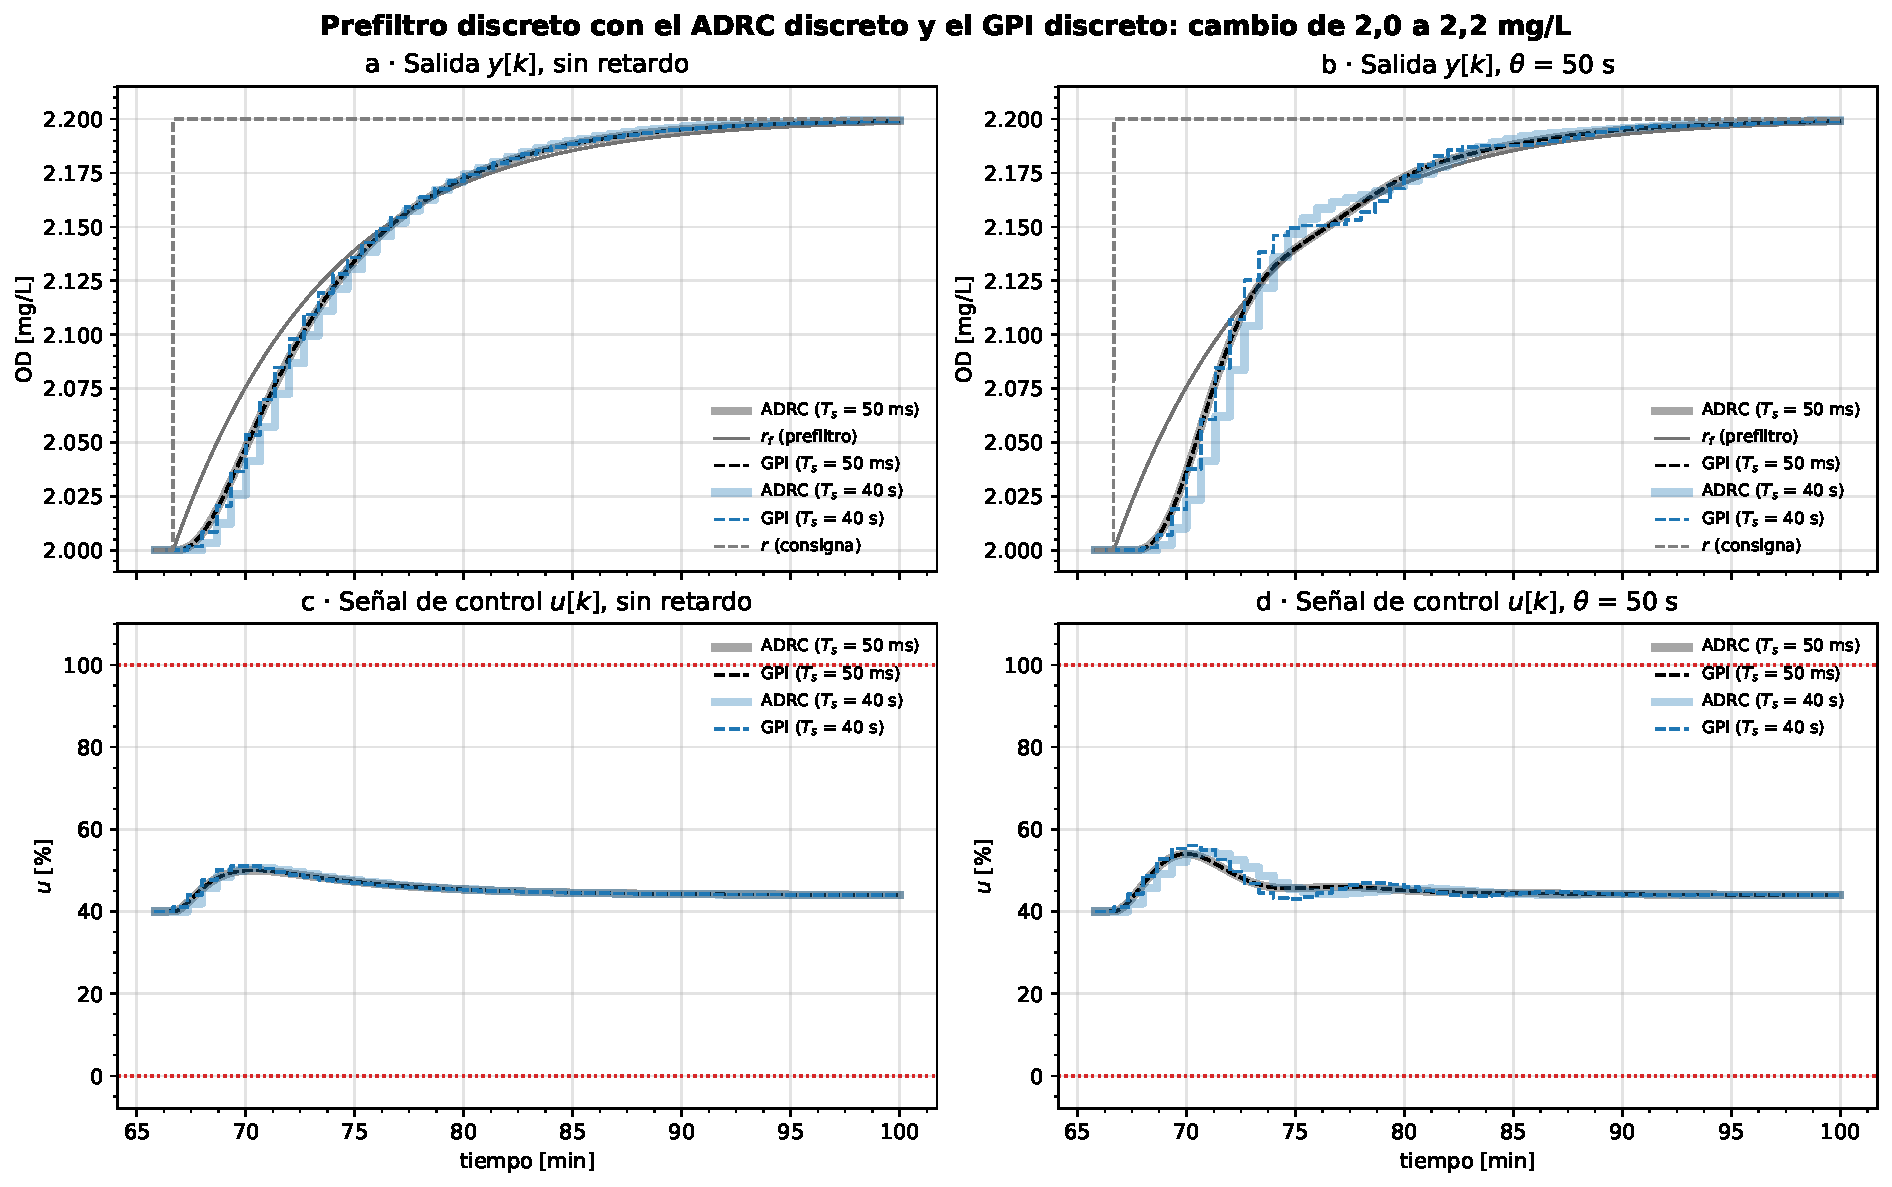
\includegraphics[width=\textwidth]{disc_prefiltro_retardo.pdf}
  \caption[Prefiltro discreto con el ADRC y el GPI discretos]{Cambio de consigna de $2{,}0$ a
    $2{,}2$~mg/L con el prefiltro discreto \eqref{eq:disc_pref_dif}, la planta exacta y el soplador
    limitado entre $0$ y $100~\%$: ADRC discreto (banda) y GPI discreto con
    $E_1 = (s + \omega_o)^2$ (discontinua), con $T_s = 50$~ms (negro) y $T_s = 40$~s (azul),
    dibujados en escalones. (a) y (c) Sin retardo; (b) y (d) con $\theta = 50$~s. Arriba, la
    salida $y[k]$; abajo, la señal de control $u[k]$.}
  \label{fig:disc_prefiltro_retardo}
\end{figure}

\begin{table}[H]
\centering
\caption[Índices del cambio de consigna con el prefiltro discreto]{Tiempo de asentamiento $t_s$ y
  pico de la señal de control $u_{\max}$ (Tabla~\ref{tab:metricas}) en el cambio de $2{,}0$ a
  $2{,}2$~mg/L de la Figura~\ref{fig:disc_prefiltro_retardo}. En ningún caso hay sobrepico.}
\label{tab:disc_prefiltro_indices}
\renewcommand{\arraystretch}{1.3}
\begin{tabular}{llcccc}
\toprule
 & & \multicolumn{2}{c}{\textbf{Sin retardo}} & \multicolumn{2}{c}{$\boldsymbol{\theta = 50}$~\textbf{s}} \\
\cmidrule(lr){3-4}\cmidrule(lr){5-6}
\textbf{Controlador} & $\boldsymbol{T_s}$ & $t_s$ [min] & $u_{\max}$ [\%] & $t_s$ [min] & $u_{\max}$ [\%] \\
\midrule
ADRC & $50$~ms & $24{,}4$ & $50{,}0$ & $24{,}7$ & $54{,}0$ \\
GPI  & $50$~ms & $24{,}4$ & $50{,}0$ & $24{,}7$ & $54{,}0$ \\
\midrule
ADRC & $40$~s  & $22{,}7$ & $50{,}5$ & $23{,}7$ & $54{,}5$ \\
GPI  & $40$~s  & $24{,}2$ & $51{,}1$ & $23{,}3$ & $56{,}1$ \\
\bottomrule
\end{tabular}
\end{table}

%--------------------------------------------------------------------
\section{Planta con retardo}
\label{sec:impl_retardo}

La planta de diseño tiene un retardo $\theta = 50$~s
\eqref{eq:ident_planta_diseno} que el observador no conoce: recibe la orden
aplicada en el mismo periodo en que se calcula, mientras que la planta solo la
ve $\theta$ segundos después. Si el retardo se conoce, una solución simple es
sincronizar el observador con la planta retrasando la orden que le entra
\cite[sec.~9.4]{herbst2024adrc}, \cite{herbst2013practical}. Con el observador
discreto \eqref{eq:disc_observador},
\begin{equation}
\widehat{\mathbf{X}}[k+1] = \bigl(\mathbf{A}_d - \mathbf{L}_d\,\mathbf{C}_d\bigr)\,\widehat{\mathbf{X}}[k]
+ \mathbf{B}_d\,b_0\,u_{\mathrm{sat}}[k - n_d] + \mathbf{L}_d\,e_y[k],
\qquad
n_d \approx \frac{\theta}{T_s} ,
\label{eq:disc_retardo}
\end{equation}
y fila por fila solo cambia la primera ecuación de \eqref{eq:disc_filas}:
\begin{equation}
\hat{x}_1[k+1] = (1 - l_{1,d})\,\hat{x}_1[k] + T_s\,\hat{x}_2[k] + T_s\,b_0\,u_{\mathrm{sat}}[k - n_d] + l_{1,d}\,e_y[k] .
\end{equation}
Las matrices, las ganancias $\mathbf{K}_d$ y $\mathbf{L}_d$ y la ley de control
\eqref{eq:disc_ley_escalar} no cambian; lo único que se añade es un registro de
las últimas $n_d$ órdenes aplicadas. Con $T_s = 50$~ms y $\theta = 50$~s,
$n_d = 1000$ muestras.

La Figura~\ref{fig:adrc_discreto_retardo} compara el ADRC discreto sin
sincronizar ($n_d = 0$) y sincronizado ($n_d = \theta/T_s$) para
$\theta = 20$, $40$, $50$, $60$ y $100$~s, con el escalón de consigna de $2{,}0$ a
$2{,}2$~mg/L y la perturbación $\varepsilon = -15~\%$ a los 40~min. Con
$\theta = 50$~s, el pico de oxígeno baja de $2{,}29$ a $2{,}24$~mg/L y la señal
de control deja de oscilar (sin sincronizar baja hasta $29~\%$; sincronizado no
pasa por debajo del $40~\%$ del estacionario). En el caso extremo de $100$~s, sin
sincronizar el lazo oscila y el soplador llega a $0$ y a $100~\%$;
sincronizado, el pico es de $2{,}26$~mg/L y la orden no pasa del $86~\%$. A
cambio, la respuesta es algo más lenta ($t_s$ de $17{,}4$ frente a $14{,}7$~min
con $\theta = 50$~s, con banda de $2~\%$ del escalón) y la caída por la
perturbación es un poco mayor ($2{,}129$ frente a $2{,}132$~mg/L), pero sin oscilación, por lo que
sincronizar el observador da mejores respuestas.

El retardo real no se conoce con exactitud: solo se obtuvo visualmente
(Sección~\ref{sec:ident_retardo}), y los diseños se hicieron con $\theta = 50$~s en la planta. Ahora
bien, sobreestimarlo es seguro: con $n_d T_s = 100$~s el pico es de $2{,}23$~mg/L y $t_s$ sube a
$20{,}7$~min. Subestimarlo no mejora, pero sigue ayudando: con $n_d T_s = 25$~s el pico es de
$2{,}26$~mg/L, frente a $2{,}29$. Por eso es mejor sobreestimar $\theta$ y elegir un valor un poco más
grande.

\begin{figure}[H]
  \centering
  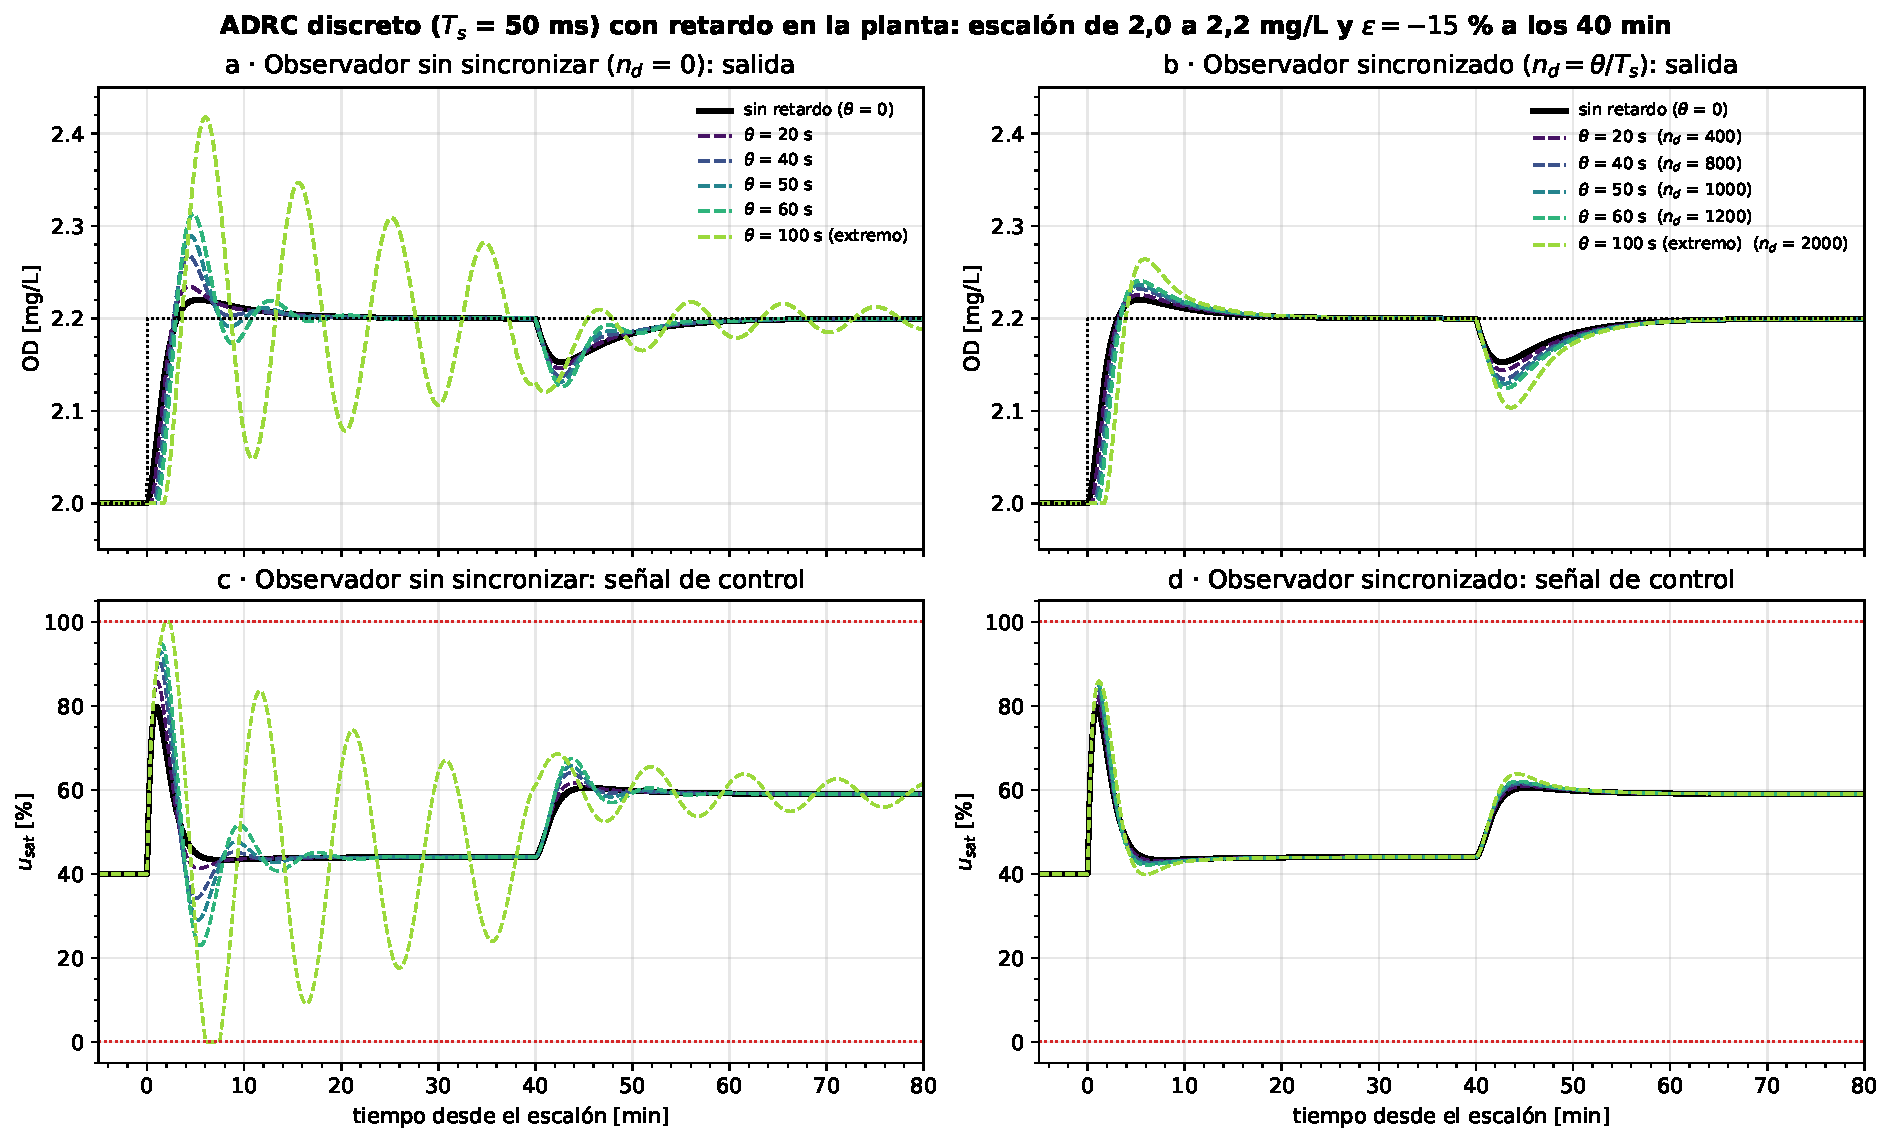
\includegraphics[width=\textwidth]{adrc_discreto_retardo.pdf}
  \caption[ADRC discreto con retardo: observador sin sincronizar y
    sincronizado]{ADRC discreto ($T_s = 50$~ms) con la planta nominal con
    retardo $\theta$ y el soplador limitado entre $0$ y $100~\%$: escalón de
    consigna de $2{,}0$ a $2{,}2$~mg/L y $\varepsilon = -15~\%$ a los 40~min.
    (a) y (c) Observador sin sincronizar ($n_d = 0$); (b) y (d) observador
    sincronizado \eqref{eq:disc_retardo}, con $n_d = \theta/T_s$. Arriba, la
    salida; abajo, la señal de control. En negro, sin retardo.}
  \label{fig:adrc_discreto_retardo}
\end{figure}

%--------------------------------------------------------------------
\section{Implementación en PLC}
\label{sec:impl_plc}
\label{sec:met_plc}
Esta sección contiene el desarrollo de los diseños propuestos anteriormente, llevando los esquemas
de saturación y algunas de las realizaciones que se obtuvieron en discreto a una forma que se pueda
implementar en un PLC. Se parte de una idea de alto nivel, donde se fundamentan las ideas
principales, y cada vez se va formalizando más con los resultados teóricos de las secciones
anteriores, hasta obtener un producto con una metodología definida para su implementación.

%--------------------------------------------------------------------
\subsection{Producto digital}
\label{subsec:plc_producto}

Todo producto digital empieza en alto nivel, como una caja negra con sus bloques de entradas y
salidas. Por dentro, cada bloque debe seguir un flujo descrito por una máquina de estados, y eso es
lo que permite integrar productos digitales en procesos industriales. En la industria se manejan
estándares con estados como inicio, arranque y parada de emergencia, entre otros. Aquí, dada la
simplicidad de los bloques, se simplificaron a solo dos estados, \texttt{RESET} y \texttt{AUTOMATIC}
(Figura~\ref{fig:plc_estados}), que ofrecen una configuración para integrarlos en procesos
industriales, ya que con ellos se puede habilitar o deshabilitar el módulo: \texttt{AUTOMATIC} lo
habilita y \texttt{RESET} lo deshabilita.


\begin{figure}[H]
  \centering
  \begin{tikzpicture}[>=Stealth, thick, font=\small,
      est/.style={draw, circle, thick, minimum size=3.2cm, text width=2.9cm, align=center,
        inner sep=0pt, fill=white, font=\footnotesize\bfseries},
      et/.style={font=\footnotesize\ttfamily, fill=white, inner sep=1.5pt, align=center}]
    \node[est] (R) at (0,0) {RESET};
    \node[est] (A) at (7.5,0) {AUTOMATIC};
    \draw[->] (R.25) to[bend left=18] node[et, above=2pt] {RESET = 0 AND Ready} (A.155);
    \draw[->] (A.205) to[bend left=18] node[et, below=2pt] {RESET = 1} (R.335);
  \end{tikzpicture}
  \caption[Máquina de estados de los bloques de función]{Máquina de estados de los bloques de
    función.}
  \label{fig:plc_estados}
\end{figure}

El producto de este trabajo son bloques de función para el PLC. Para el control
son tres: el ADRC basado en observador, el GPI con sus ganancias y el GPI con
los anchos de banda (Tablas~\ref{tab:plc_adrc_eso}, \ref{tab:plc_gpi} y \ref{tab:plc_adrc_gpi}). El
ADRC se sintoniza con $\omega_c$, $\omega_o$ y $b_0$
(Sección~\ref{subsec:sintonia}). El GPI recibe directamente $k_0$, $k_1$, $k_2$
y $b_0$: si se conocen $\omega_c$ y $\omega_o$, las ganancias salen de
\eqref{eq:eso2gpi} y los dos bloques dan el mismo lazo; o si se quiere se sintoniza
como un PI con filtro (Figura~\ref{fig:gpi_pi_filtro}), con $k_1$ y $k_0$ como
acciones proporcional e integral y $k_2$ como polo del filtro. En ese caso nada
garantiza la estabilidad, así que el bloque verifica que $k_0, k_1, k_2 > 0$ y
$k_2 k_1 > k_0$, la condición de Routh--Hurwitz de
$\Delta(s) = s^3 + k_2 s^2 + k_1 s + k_0$ con la planta de diseño, y si no se
cumple conserva las ganancias anteriores. \texttt{ADRC\_GPI} recibe $\omega_c$, $\omega_o$
y $b_0$, calcula $k_0$, $k_1$ y $k_2$ con \eqref{eq:eso2gpi} y usa
$E_1(s) = (s + \omega_o)^2$ \eqref{eq:aw_gpi_wo}, con lo que se comporta igual que el
ADRC también cuando satura. La
consigna y la medida
entran como \texttt{SET\_POINT} y \texttt{ACTUAL}, y dentro se calcula la resta que da el error de
seguimiento; la salida \texttt{U} es la orden al soplador, ya limitada entre \texttt{U\_MIN} y
\texttt{U\_MAX}.

El estado \texttt{RESET} funciona como el de un PID industrial, que lleva la salida a un valor fijo
(\texttt{Y\_OFFSET}) y borra la parte integral: aquí la salida va a cero, dentro de los límites, y los estados se reinician. Las
ganancias solo se actualizan en \texttt{RESET}, y el bloque sale de ese estado cuando ya tiene
parámetros válidos (\texttt{Ready}). Seguidamente, Cada tabla muestra el símbolo del bloque, qué hace cada entrada
y salida, y las ecuaciones que implementa; el código está en el repositorio del Anexo~\ref{anx:st}. Todas las entradas
son reales salvo \texttt{TS}, de tipo \texttt{TIME}, y \texttt{RESET}, que es booleana.

% bloque de funcion: \bloqueplc{x}{nombre}{alto}{entradas}{salidas}
\newcommand{\bloqueplc}[5]{%
  \begin{scope}[xshift=#1 cm]
    \draw (0,0) rectangle (3.2,#3);
    \node[font=\ttfamily] at (1.6,-0.35) {#2};
    \draw[thin] (0,-0.7) -- (3.2,-0.7);
    \foreach \i/\pin/\sen in {#4} {
      \draw[->] (-0.6,-0.6-0.55*\i) node[left] {\sen} -- (0,-0.6-0.55*\i);
      \node[right, font=\ttfamily\footnotesize] at (0,-0.6-0.55*\i) {\pin};
    }
    \foreach \i/\pin/\sen in {#5} {
      \draw[->] (3.2,-0.6-0.55*\i) -- (3.8,-0.6-0.55*\i) node[right] {\sen};
      \node[left, font=\ttfamily\footnotesize] at (3.2,-0.6-0.55*\i) {\pin};
    }
  \end{scope}%
}

% ficha de un bloque: \fichaplc{nombre}{etiqueta}{alto}{entradas}{salidas}{filas de entradas}{fila de salida}{descripcion}{ecuaciones}
\newcommand{\fichaplc}[9]{%
  \begin{table}[H]
  \centering
  \caption[Bloque \texttt{#1}]{Bloque de función \texttt{#1}.}
  \label{#2}
  \footnotesize
  \renewcommand{\arraystretch}{1.1}
  \begin{tabular}{@{}p{0.255\linewidth}p{0.465\linewidth}p{0.23\linewidth}@{}}
  \toprule
  \textbf{Símbolo} & \textbf{Entradas y salida} & \textbf{Descripción} \\
  \midrule
  \centering
  \begin{tikzpicture}[>=Stealth, thick, font=\small, scale=0.7, transform shape,
      baseline=(current bounding box.north)]
    \bloqueplc{0}{#1}{#3}{#4}{#5}
  \end{tikzpicture}
  &
  \begin{tabular}[t]{@{}p{1.72cm}@{\hspace{5pt}}>{\raggedright\arraybackslash}p{5.8cm}@{}}
  #6
  \cmidrule{1-2}
  #7
  \end{tabular}
  &
  \begin{minipage}[t]{\linewidth}
    \raggedright #8\par\medskip
    \textbf{Ecuaciones}\par
    #9
  \end{minipage} \\
  \bottomrule
  \end{tabular}
  \end{table}%
}

\fichaplc{ADRC\_ESO}{tab:plc_adrc_eso}{-5.85}
  {1/SET\_POINT/$r$, 2/ACTUAL/$y$, 3/WC/$\omega_c$, 4/WO/$\omega_o$, 5/B0/$b_0$, 6/TS/$T_s$,
    7/U\_MIN/$u_{\min}$, 8/U\_MAX/$u_{\max}$, 9/RESET/\textit{reset}}{1/U/$u_{\mathrm{sat}}$}
  {\texttt{SET\_POINT} & Consigna en mg/L. \\
   \texttt{ACTUAL} & Medida en mg/L. \\
   \texttt{WC} & Ancho de banda del controlador en rad/s; mayor que 0. \\
   \texttt{WO} & Ancho de banda del observador en rad/s; mayor que \texttt{WC}. \\
   \texttt{B0} & Ganancia en mg/(L$\cdot$s$\cdot$\%); positiva. \\
   \texttt{TS} & Periodo de la tarea cíclica (\texttt{TIME}). \\
   \texttt{U\_MIN} & Mínimo de \texttt{U}; por defecto, 0. \\
   \texttt{U\_MAX} & Máximo de \texttt{U}; por defecto, 100. \\
   \texttt{RESET} & Con \texttt{TRUE} lleva \texttt{U} a cero dentro de los límites, reinicia el observador
     ($\hat{x}_1 = 0$, $\hat{x}_2 = -b_0\,u_{\mathrm{sat}}$) y carga los parámetros. Con
     \texttt{FALSE} controla. \\}
  {\texttt{U} & Orden al soplador, ya limitada.}
  {ADRC basado en el error con observador de estado extendido. Estima el error y la perturbación
    total, y la ley de control cancela esa perturbación.}
  {Observador: \eqref{eq:disc_filas_retardos}\\
    Ley de control: \eqref{eq:disc_ley_escalar}\\
    Ganancias: \eqref{eq:disc_ganancias_wc_wo}}

\fichaplc{GPI}{tab:plc_gpi}{-6.4}
  {1/SET\_POINT/$r$, 2/ACTUAL/$y$, 3/K0/$k_0$, 4/K1/$k_1$, 5/K2/$k_2$, 6/B0/$b_0$, 7/TS/$T_s$,
    8/U\_MIN/$u_{\min}$, 9/U\_MAX/$u_{\max}$, 10/RESET/\textit{reset}}{1/U/$u_{\mathrm{sat}}$}
  {\texttt{SET\_POINT} & Consigna en mg/L. \\
   \texttt{ACTUAL} & Medida en mg/L. \\
   \texttt{K0} & Acción integral; mayor que 0. \\
   \texttt{K1} & Acción proporcional; mayor que 0. \\
   \texttt{K2} & Polo del filtro; mayor que 0 y con $k_2 k_1 > k_0$. \\
   \texttt{B0} & Ganancia en mg/(L$\cdot$s$\cdot$\%); positiva. \\
   \texttt{TS} & Periodo de la tarea cíclica (\texttt{TIME}). \\
   \texttt{U\_MIN} & Mínimo de \texttt{U}; por defecto, 0. \\
   \texttt{U\_MAX} & Máximo de \texttt{U}; por defecto, 100. \\
   \texttt{RESET} & Con \texttt{TRUE} lleva \texttt{U} a cero dentro de los límites, pone en cero los
     retardos de $-e_y$, deja los de $v$ y $u_{\mathrm{sat}}$ en esa orden y carga los parámetros. Con
     \texttt{FALSE} controla. \\}
  {\texttt{U} & Orden al soplador, ya limitada.}
  {GPI sintonizado con sus ganancias. Si estas salen de $\omega_c$ y $\omega_o$, da el mismo lazo que
    el ADRC; si no se conocen, se sintoniza como un PI con filtro.}
  {Ley en retardos: \eqref{eq:disc_gpi_fd1}\\
    Coeficientes: Tabla~\ref{tab:disc_gpi_coef}\\
    Anti-\emph{windup}: \eqref{eq:aw_gpi}}

\fichaplc{ADRC\_GPI}{tab:plc_adrc_gpi}{-5.85}
  {1/SET\_POINT/$r$, 2/ACTUAL/$y$, 3/WC/$\omega_c$, 4/WO/$\omega_o$, 5/B0/$b_0$, 6/TS/$T_s$,
    7/U\_MIN/$u_{\min}$, 8/U\_MAX/$u_{\max}$, 9/RESET/\textit{reset}}{1/U/$u_{\mathrm{sat}}$}
  {\texttt{SET\_POINT} & Consigna en mg/L. \\
   \texttt{ACTUAL} & Medida en mg/L. \\
   \texttt{WC} & Ancho de banda del controlador en rad/s; mayor que 0. \\
   \texttt{WO} & Ancho de banda del observador en rad/s; mayor que \texttt{WC}. \\
   \texttt{B0} & Ganancia en mg/(L$\cdot$s$\cdot$\%); positiva. \\
   \texttt{TS} & Periodo de la tarea cíclica (\texttt{TIME}). \\
   \texttt{U\_MIN} & Mínimo de \texttt{U}; por defecto, 0. \\
   \texttt{U\_MAX} & Máximo de \texttt{U}; por defecto, 100. \\
   \texttt{RESET} & Con \texttt{TRUE} lleva \texttt{U} a cero dentro de los límites, pone en cero los
     retardos de $-e_y$, deja los de $v$ y $u_{\mathrm{sat}}$ en esa orden y carga los parámetros. Con
     \texttt{FALSE} controla. \\}
  {\texttt{U} & Orden al soplador, ya limitada.}
  {GPI sintonizado con $\omega_c$, $\omega_o$ y $b_0$, igual que el ADRC. Calcula sus coeficientes por
    dentro y se comporta como el ADRC también cuando satura.}
  {Ley en retardos: \eqref{eq:disc_gpi_fd1}\\
    Coeficientes: Tabla~\ref{tab:disc_gpi_coef}\\
    Anti-\emph{windup}: \eqref{eq:aw_gpi_wo}\\
    Ganancias: \eqref{eq:eso2gpi}}

La consigna puede pasar antes por uno de tres bloques (Tablas~\ref{tab:plc_prefilter_gpi}, \ref{tab:plc_prefilter_adrc} y \ref{tab:plc_bezier}), cuya salida
va a \texttt{SET\_POINT} del controlador. \texttt{PREFILTER\_GPI} y \texttt{PREFILTER\_ADRC} son el mismo
prefiltro \eqref{eq:disc_pref_dif}: el primero calcula $\alpha_f$ y $\beta_f$ con $k_0$ y $k_1$, y el
segundo con $\omega_c$ y $\omega_o$. \texttt{BEZIER\_REF} genera la referencia de Bézier
\eqref{eq:bz_horner} con duración $t_f$, también de tipo \texttt{TIME}, y replanifica en cada cambio
de consigna (Sección~\ref{subsec:bz_replanificacion}). El usuario elige $t_f$, que se aplica en el
siguiente cambio de consigna. Con \texttt{RESET} la salida de los tres sigue a \texttt{ACTUAL}, y al
soltarlo la maniobra arranca desde la medida, de modo que el filtro recibe el escalón $r - y$. Su
\texttt{RESET} se conecta al del controlador, porque si la referencia siguiera hacia la consigna
mientras el controlador no actúa, este saltaría al volver a \texttt{AUTOMATIC}. Todos reciben $T_s$ en \texttt{TS}, de tipo \texttt{TIME}, que debe ser
el periodo de la tarea cíclica. La Tabla~\ref{tab:plc_plant} presenta además el bloque \texttt{PLANT}, que
sirve para probar los anteriores sin conectarlos al proceso.

\fichaplc{PREFILTER\_GPI}{tab:plc_prefilter_gpi}{-4.2}
  {1/SET\_POINT/$r$, 2/ACTUAL/$y$, 3/K0/$k_0$, 4/K1/$k_1$, 5/TS/$T_s$, 6/RESET/\textit{reset}}{1/Y/$r_f$}
  {\texttt{SET\_POINT} & Consigna sin filtrar, en mg/L. \\
   \texttt{ACTUAL} & Medida en mg/L; de ahí arranca el filtro al soltar \texttt{RESET}. \\
   \texttt{K0} & Ganancia del filtro; mayor que 0. \\
   \texttt{K1} & Ganancia del filtro; mayor que 0. \\
   \texttt{TS} & Periodo de la tarea cíclica (\texttt{TIME}). \\
   \texttt{RESET} & Con \texttt{TRUE} la salida sigue a \texttt{ACTUAL} y se cargan los parámetros. Con
     \texttt{FALSE} filtra desde ese valor. Se conecta al \texttt{RESET} del controlador. \\}
  {\texttt{Y} & Consigna filtrada; va a \texttt{SET\_POINT} del controlador.}
  {Filtro de primer orden de la consigna, con constante de tiempo $k_1/k_0$. Cancela el cero del
    lazo, así que quita el sobrepico y reduce el pico de la orden, sin cambiar el rechazo de
    perturbaciones.}
  {Prefiltro: \eqref{eq:pref_f}\\
    En diferencias: \eqref{eq:disc_pref_dif}\\
    Coeficientes: \eqref{eq:disc_pref_tf}}

\fichaplc{PREFILTER\_ADRC}{tab:plc_prefilter_adrc}{-4.2}
  {1/SET\_POINT/$r$, 2/ACTUAL/$y$, 3/WC/$\omega_c$, 4/WO/$\omega_o$, 5/TS/$T_s$, 6/RESET/\textit{reset}}{1/Y/$r_f$}
  {\texttt{SET\_POINT} & Consigna sin filtrar, en mg/L. \\
   \texttt{ACTUAL} & Medida en mg/L; de ahí arranca el filtro al soltar \texttt{RESET}. \\
   \texttt{WC} & Ancho de banda del controlador en rad/s; mayor que 0. \\
   \texttt{WO} & Ancho de banda del observador en rad/s; mayor que \texttt{WC}. \\
   \texttt{TS} & Periodo de la tarea cíclica (\texttt{TIME}). \\
   \texttt{RESET} & Con \texttt{TRUE} la salida sigue a \texttt{ACTUAL} y se cargan los parámetros. Con
     \texttt{FALSE} filtra desde ese valor. Se conecta al \texttt{RESET} del controlador. \\}
  {\texttt{Y} & Consigna filtrada; va a \texttt{SET\_POINT} del controlador.}
  {El mismo prefiltro de la Tabla~\ref{tab:plc_prefilter_gpi}, sintonizado con $\omega_c$ y $\omega_o$.
    Su constante de tiempo es $(\omega_o + 2\omega_c)/(\omega_c\,\omega_o)$.}
  {Prefiltro: \eqref{eq:pref_f}\\
    En diferencias: \eqref{eq:disc_pref_dif}\\
    Coeficientes: \eqref{eq:disc_pref_tf}\\
    Ganancias: \eqref{eq:eso2gpi}}

\fichaplc{BEZIER\_REF}{tab:plc_bezier}{-3.65}
  {1/SET\_POINT/$r$, 2/ACTUAL/$y$, 3/TF/$t_f$, 4/TS/$T_s$, 5/RESET/\textit{reset}}{1/Y/$y^*$}
  {\texttt{SET\_POINT} & Consigna en mg/L; cada cambio replanifica la referencia. \\
   \texttt{ACTUAL} & Medida en mg/L; de ahí arranca la maniobra al soltar \texttt{RESET}. \\
   \texttt{TF} & Duración de la maniobra (\texttt{TIME}); se lee en cada cambio de consigna. Por
     defecto, 20 min. \\
   \texttt{TS} & Periodo de la tarea cíclica (\texttt{TIME}). \\
   \texttt{RESET} & Con \texttt{TRUE} la salida sigue a \texttt{ACTUAL} y se cargan los parámetros. Con
     \texttt{FALSE} la maniobra vuelve a empezar desde la medida. Se conecta al \texttt{RESET} del
     controlador. \\}
  {\texttt{Y} & Referencia suave; va a \texttt{SET\_POINT} del controlador.}
  {Genera una referencia de Bézier que llega a la consigna en $t_f$, sin saltos de valor ni de
    pendiente, para reducir el esfuerzo de control.}
  {Coeficientes: \eqref{eq:bz_c}\\
    Referencia: \eqref{eq:bz_horner}\\
    Replanificación: Sección~\ref{subsec:bz_replanificacion}}

\fichaplc{PLANT}{tab:plc_plant}{-3.1}
  {1/U/$u$, 2/K\_DC/$k_{dc}$, 3/TAU/$\tau$, 4/TS/$T_s$}{1/Y/$y$}
  {\texttt{U} & Entrada de la planta; se conecta a \texttt{U} del controlador. \\
   \texttt{K\_DC} & Ganancia estática en mg/(L$\cdot$\%). \\
   \texttt{TAU} & Constante de tiempo en s. \\
   \texttt{TS} & Periodo de la tarea cíclica (\texttt{TIME}). \\}
  {\texttt{Y} & Oxígeno simulado; se conecta a \texttt{ACTUAL}.}
  {Planta de primer orden discretizada con Tustin, para probar los bloques en el PLC. Se llama después
    del controlador y no tiene \texttt{RESET}.}
  {Coeficientes $\alpha_g$ y $\beta_g$: Tabla~\ref{tab:disc_gpi_coef}}

%--------------------------------------------------------------------
\subsection{Implementación en lenguajes}
\label{subsec:plc_lenguajes}

Las realizaciones discretas de las Figuras~\ref{fig:adrc_discreto_retardos} y
\ref{fig:disc_formas_directas} solo tienen sumas, ganancias y retardos. Las sumas y las ganancias
existen en todos los lenguajes de la norma IEC~61131-3 \cite{iec61131}, así que lo único que hay que
resolver es el retardo $z^{-1}$, es decir, guardar un valor para usarlo en el ciclo siguiente. Incluso
hay plataformas que ya traen un bloque de retardo. Aun así, se puede construir con cualquiera de los lenguajes de la
norma, y la
regla es la misma en todos: la variable debe conservar su valor entre ciclos, por lo que va en un
bloque de función o en un programa y no en una función; se lee antes de escribirla, y en una cadena
de retardos se actualiza primero el más viejo. La norma define los lenguajes textuales, como ST, y
los gráficos FBD y LD, además de SFC para organizar secuencias; el CFC no hace parte de la norma,
sino que es un editor gráfico que CODESYS, y por lo tanto ctrlX PLC, ofrece como extensión del FBD
\cite{codesysHelp}. La Tabla~\ref{tab:plc_lenguajes} muestra cómo se hace el retardo en cada uno. En
este trabajo se usó ST para los bloques y CFC solo para visualizarlos.

\begin{table}[H]
\centering
\caption[Retardo $z^{-1}$ en cada lenguaje]{Retardo $z^{-1}$ en cada lenguaje, con
  $x_1 = x[k-1]$ y $x_2 = x[k-2]$.}
\label{tab:plc_lenguajes}
\footnotesize
\renewcommand{\arraystretch}{1.2}
\begin{tabular}{@{}>{\raggedright\arraybackslash}p{0.17\linewidth}p{0.32\linewidth}>{\raggedright\arraybackslash}p{0.45\linewidth}@{}}
\toprule
\textbf{Lenguaje} & \textbf{Retardo} & \textbf{Cómo funciona} \\
\midrule
Texto estructurado (ST) &
  \texttt{x\_2 := x\_1;}\newline\texttt{x\_1 := x;} &
  Las asignaciones se ejecutan en orden. Se escriben al final, después de calcular la salida, y
  primero la del retardo más viejo. Así están hechos los bloques de este trabajo. \\
\addlinespace
Diagrama de bloques de función (FBD) &
  \begin{tikzpicture}[>=Stealth, thick, font=\scriptsize\ttfamily, baseline=(current bounding box.north)]
    \foreach \y/\a/\b in {0/x\_1/x\_2, -0.8/x/x\_1} {
      \draw (0,\y) rectangle (1.1,\y-0.6);
      \node at (0.55,\y-0.3) {MOVE};
      \draw[->] (-0.4,\y-0.3) node[left] {\a} -- (0,\y-0.3);
      \draw[->] (1.1,\y-0.3) -- (1.5,\y-0.3) node[right] {\b};
    }
  \end{tikzpicture} &
  Dos bloques \texttt{MOVE} en las últimas redes. Las redes se ejecutan de arriba hacia abajo, así
  que las anteriores leen el valor del ciclo pasado. \\
\addlinespace
Diagrama de escalera (LD) &
  \begin{tikzpicture}[>=Stealth, thick, font=\scriptsize\ttfamily, baseline=(current bounding box.north)]
    \draw[line width=1.2pt] (0,0) -- (0,-0.9);
    \draw[line width=1.2pt] (3.5,0) -- (3.5,-0.9);
    \draw (0,-0.25) -- (1.1,-0.25);
    \draw (2.4,-0.25) -- (3.5,-0.25);
    \draw (1.1,0) rectangle (2.4,-0.9);
    \node at (1.75,-0.25) {MOVE};
    \draw (0.8,-0.65) node[left] {x} -- (1.1,-0.65);
    \draw (2.4,-0.65) -- (2.7,-0.65) node[right] {x\_1};
  \end{tikzpicture} &
  Un escalón con \texttt{MOVE}, debajo de los escalones que leen el valor, porque se ejecutan de
  arriba hacia abajo. Las sumas y ganancias van en bloques \texttt{ADD} y \texttt{MUL}. \\
\addlinespace
SFC, derivado del GRAFCET &
  \begin{tikzpicture}[>=Stealth, thick, font=\scriptsize\ttfamily, baseline=(current bounding box.north)]
    \draw (0.875,0.25) -- (0.875,0);
    \draw (0,0) rectangle (1.75,-0.5);
    \draw (0.05,-0.05) rectangle (1.7,-0.45);
    \node at (0.875,-0.25) {AUTOMATIC};
    \draw (1.75,-0.25) -- (2.0,-0.25);
    \draw (2.0,0) rectangle (3.5,-0.5);
    \draw (2.35,0) -- (2.35,-0.5);
    \node at (2.175,-0.25) {N};
    \node at (2.925,-0.25) {DELAYS};
    \draw (0.875,-0.5) -- (0.875,-0.95);
    \draw (0.675,-0.75) -- (1.075,-0.75);
    \node[right] at (1.075,-0.75) {RESET};
  \end{tikzpicture} &
  Organiza la secuencia, no calcula: el retardo va dentro de la acción de la etapa, escrita en ST,
  FBD o LD. Con el calificador \texttt{N} la acción corre mientras la etapa esté activa
  \cite{codesysHelp}. Las etapas pueden ser las de la Figura~\ref{fig:plc_estados}. \\
\bottomrule
\end{tabular}
\end{table}

%--------------------------------------------------------------------
\subsection{Implementación en software}
\label{subsec:plc_software}

Los bloques se escribieron en ST en la plataforma ctrlX WORKS de Bosch Rexroth, que está basada en
CODESYS. Para armar el lazo se usó
CFC (\emph{Continuous Function Chart}), porque en ese lenguaje se ven los bloques y sus conexiones
de una forma más fácil, pero por dentro cada bloque sigue siendo ST. La
Figura~\ref{fig:plc_codesys} muestra las instancias de los bloques ya creados.

\begin{figure}[tbp]
  \centering
  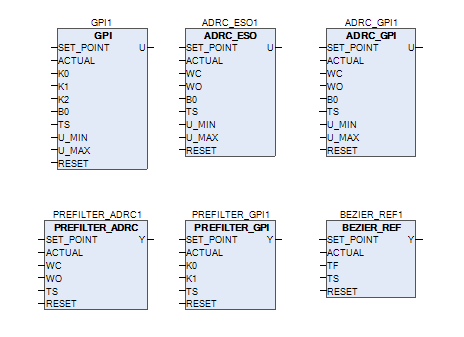
\includegraphics[width=0.68\textwidth]{codesys_bloques.png}
  \caption[Instancias de los bloques en CODESYS]{Instancias de los bloques de función}
  \label{fig:plc_codesys}
\end{figure}

Para probar el lazo completo se conectó cada combinación de consigna y controlador al bloque
\texttt{PLANT}, configurado como la planta de diseño, $\tau = 1200$~s (20~min) y $k_{dc} = 0{,}05$~mg/(L$\cdot$\%),
y con la misma sintonía de las secciones anteriores: $\omega_c = 4/\tau$, $\omega_o = 5\,\omega_c$,
$b_0 = k_{dc}/\tau$ y $T_s = 50$~ms. La
Figura~\ref{fig:plc_en_linea} muestra dos de estas pruebas en línea, con el sistema ya en estacionario: la orden de
$40~\%$ sostiene $2$~mg/L y la de $44~\%$ sostiene $2{,}2$~mg/L, que es lo que da $k_{dc}$. Así se valida que el comportamiento sea el
correspondiente.

\begin{figure}[H]
  \centering
  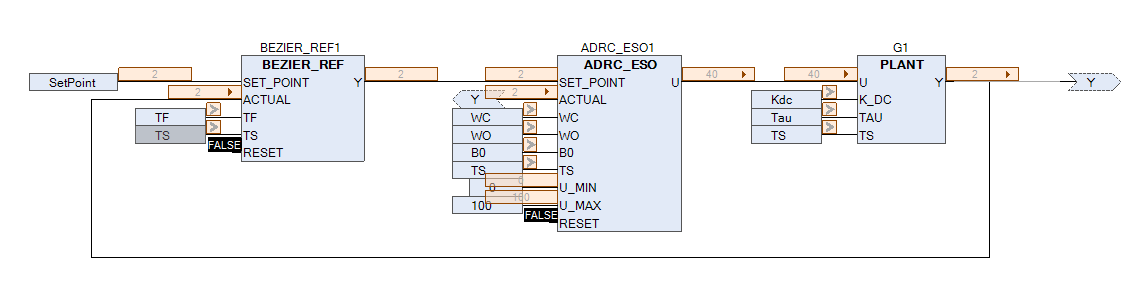
\includegraphics[width=\textwidth]{codesys_bezier_eso_en_linea.png}\\[6pt]
  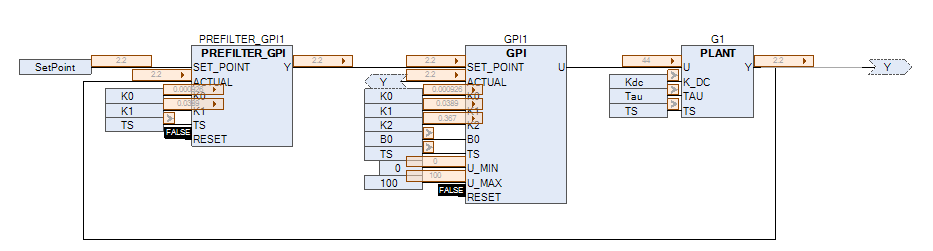
\includegraphics[width=\textwidth]{codesys_prefilter_gpi_en_linea.png}
  \caption[Lazos en línea en CODESYS]{Lazos en línea con el bloque \texttt{PLANT}. Arriba, \texttt{BEZIER\_REF} y \texttt{ADRC\_ESO} con consigna de $2$~mg/L; abajo,
    \texttt{PREFILTER\_GPI} y \texttt{GPI} con consigna de $2{,}2$~mg/L.}
  \label{fig:plc_en_linea}
\end{figure}

La Figura~\ref{fig:plc_trazas} muestra las trazas registradas por el PLC en dos corridas, con cambios
de consigna de $0$ a $2$~mg/L y de $2$ a $2{,}2$~mg/L, y la Tabla~\ref{tab:plc_trazas} resume la
información. Con Bézier se usó $t_f = 2400$~s (40~min) para el primer cambio de referencia y $t_f = 1200$~s (20~min)
para el segundo. La curva de Bézier no lleva el control a la saturación en el primer escalón, que era
el que requería mayor esfuerzo, y deja un sobrepico de $4{,}4~\%$ en el segundo, porque el cero sigue
en el lazo. Aun así, no se pierde robustez ni rechazo, ya que la curva de Bézier solo ayuda a que la
salida llegue a la referencia suavemente. El prefiltro no tiene sobrepico en ninguno de los dos, pero en el escalón
grande la orden llega a $100~\%$ durante $30{,}6$~s, por lo que reducir $\omega_c$ a $3/\tau$ (tres veces más rápido que la planta en lazo abierto) ayudaría a no saturar, y $4/\tau$ sería el límite. En el escalón pequeño, el prefiltro con el ADRC se
asienta en $24{,}5$~min con una orden máxima de $50{,}1~\%$, prácticamente los mismos valores de la
Tabla~\ref{tab:disc_prefiltro_indices} para $T_s = 50$~ms sin retardo.

\begin{figure}[H]
  \centering
  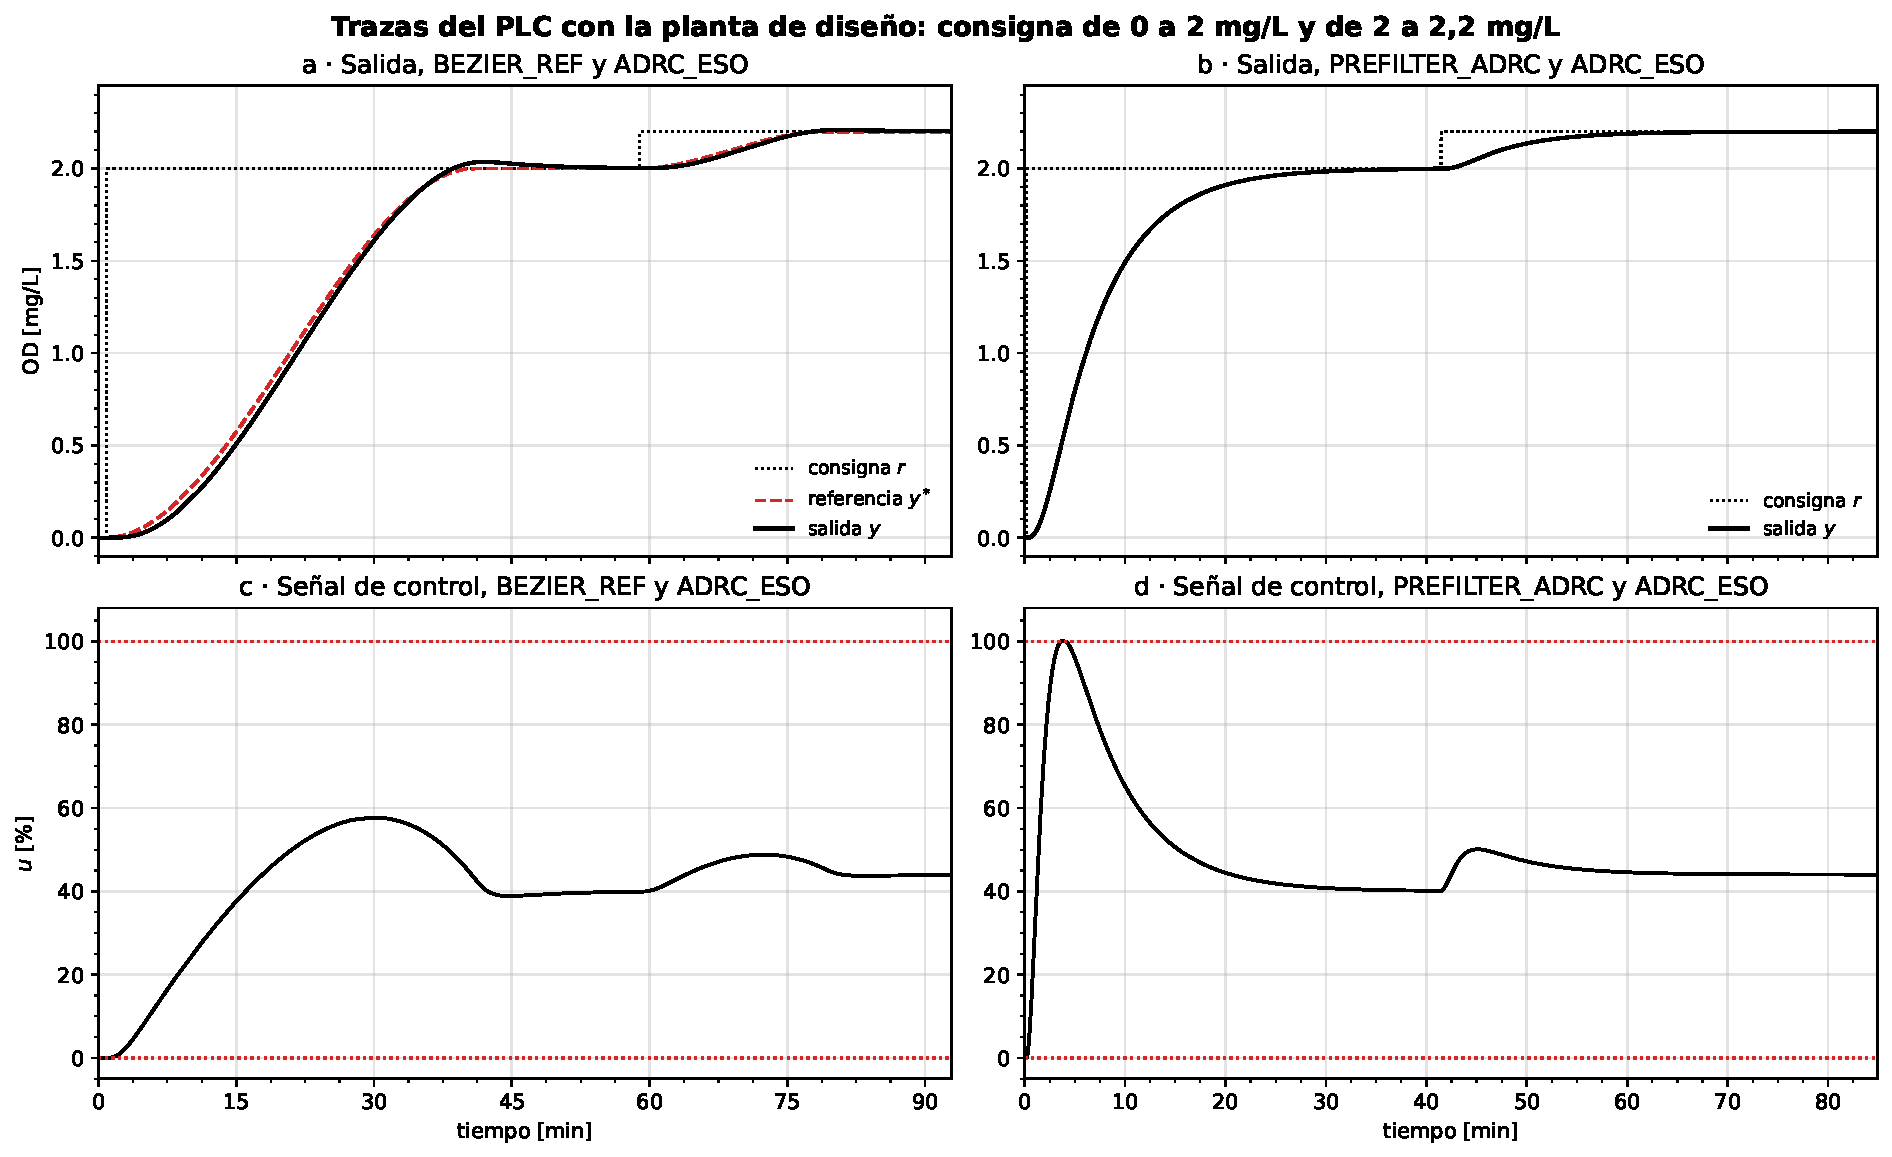
\includegraphics[width=\textwidth]{plc_trazas.pdf}
  \caption[Trazas del PLC con Bézier y con prefiltro]{Trazas registradas por el PLC con el bloque
    \texttt{PLANT} configurado como la planta de diseño. (a) y (c) \texttt{BEZIER\_REF} con
    \texttt{ADRC\_ESO}. (b) y (d) \texttt{PREFILTER\_ADRC} con \texttt{ADRC\_ESO}.}
  \label{fig:plc_trazas}
\end{figure}

\begin{table}[H]
\centering
\caption[Indicadores de las trazas del PLC]{Indicadores de las trazas de la
  Figura~\ref{fig:plc_trazas}, medidos desde cada cambio de consigna.}
\label{tab:plc_trazas}
\renewcommand{\arraystretch}{1.2}
\begin{tabular}{llccc}
\toprule
\textbf{Lazo} & \textbf{Consigna [mg/L]} & \textbf{Sobrepico} & \textbf{$t_s$ ($2~\%$)} & \textbf{$u$ máxima} \\
\midrule
\texttt{BEZIER\_REF} y \texttt{ADRC\_ESO} & $0 \to 2$ & $1{,}8~\%$ & $36{,}3$~min & $57{,}7~\%$ \\
 & $2 \to 2{,}2$ & $4{,}4~\%$ & $27{,}4$~min & $48{,}8~\%$ \\
\addlinespace
\texttt{PREFILTER\_ADRC} y \texttt{ADRC\_ESO} & $0 \to 2$ & $0~\%$ & $24{,}4$~min & $100~\%$ \\
 & $2 \to 2{,}2$ & $0~\%$ & $24{,}5$~min & $50{,}1~\%$ \\
\bottomrule
\end{tabular}
\end{table}



%--------------------------------------------------------------------
\section{Resumen: recetas de implementación}
\label{sec:impl_resumen}

En esta sección se organiza lo desarrollado para implementar el ADRC y el GPI dentro de un dispositivo
digital como un PLC, en cuatro recetas: el ADRC con observador de estado extendido a nivel general, el
GPI Robusto, los aspectos prácticos de implementación y, por último, la implementación en el PLC. Cada paso
dice qué hacer y remite a la ecuación o la sección donde está el detalle.

\subsection{Implementación del ADRC con observador de estado extendido: caso general}

\begin{recuadro}{Receta 1}
\begin{enumerate}\setlength{\itemsep}{2pt}
  \item \textbf{Modelo de la planta.} Con un experimento cerca del punto de operación
  (Figura~\ref{fig:ident_escalon_ref}) se mide cuánto cambia la salida ante un cambio en la entrada, y
  de ahí se hallan el orden $n$, la ganancia $k_{dc}$ y la constante de tiempo $\tau$ o el ancho de
  banda. Con eso se obtiene $b_0$, que para primer orden es $k_{dc}/\tau$ \eqref{eq:car_b0} y para
  otros órdenes sale de \cite[tabla~3.1]{herbst2024adrc}. Luego se reescribe la planta sobre el error:
  con $u_0 = b_0\,u$, la dinámica del error queda como una cadena de $n$ integradores excitada por
  $u_0 + \xi$ \eqref{eq:error_norm}.
  \item \textbf{Perturbación.} Se elige el modelo interno según la señal que se desea rechazar o seguir:
  escalones $1/s$ ($m = 1$), rampas $1/s^2$ ($m = 2$) o polinomios de mayor grado. Las perturbaciones
  que no siguen ese modelo también se rechazan, en la medida en que lo permita el ancho de banda del
  observador.
  \item \textbf{Sistema aumentado y observador.} Se juntan la cadena de integradores y el modelo
  interno en un solo sistema de orden $n + m$ \eqref{eq:aumentado}, cuyos estados son el error, sus
  derivadas y la perturbación con sus derivadas \eqref{eq:aumentado_matrices}. Sobre él se arma el
  observador \eqref{eq:observador}, que recibe el error medido y la orden $u_0$ y estima todos esos
  estados \eqref{eq:observador_matrices}.
  \item \textbf{Sintonía del controlador.} Se necesitan $n$ ganancias, $k_{p_1}, \dots, k_{p_n}$
  (Sección~\ref{subsec:ley}). Se pueden ubicar los polos donde se quiera con la fórmula de Ackermann
  \eqref{eq:ackermann_K}, o ponerlos todos en $-\omega_c$ con la sintonía por ancho de banda
  \eqref{eq:sintonia_l}, donde $\omega_c$ define qué tan rápido llega el sistema al estacionario. En
  la planta se eligió $\omega_c = 4/\tau$, cuatro veces más rápido que la planta en lazo abierto, que
  es la dinámica final que queda.
  \item \textbf{Sintonía del observador.} Se necesitan $n + m$ ganancias, que estiman tanto los
  estados de la planta como la perturbación: con Ackermann para el observador \eqref{eq:ackermann_L},
  o por ancho de banda \eqref{eq:sintonia_l}, con todos los polos en $-\omega_o$, donde $\omega_o$
  está entre $3$ y $10$ veces $\omega_c$ \cite[sec.~3.3]{herbst2024adrc}. En la planta se eligió
  $\omega_o = 5\,\omega_c$.
\end{enumerate}
\end{recuadro}

\subsection{Implementación del GPI robusto}

\begin{recuadro}{Receta 2}
\begin{enumerate}\setlength{\itemsep}{2pt}
  \item \textbf{Modelo de la planta.} Igual que en el ADRC: el orden $n$ y la ganancia $b_0$
  \eqref{eq:car_b0}, con el mismo experimento cerca del punto de operación.
  \item \textbf{Perturbación e integradores.} Se elige la señal que se quiere rechazar, es decir, el
  modelo interno $D_A = s^m$ del lazo cerrado escrito como fracción \eqref{eq:gpi_lazo_general}. El
  controlador se construye solo con integrales del error y de la señal de control, reconstruyendo el
  error en vez de observarlo (Sección~\ref{subsec:gpi_integradores}); para $n = m = 1$ queda un PI con
  un polo adicional, dado por el filtro \eqref{eq:gpi_ley}, y la Tabla~\ref{tab:gpi_conteo} resume los
  controladores que se obtienen según $n$ y $m$.
  \item \textbf{Sintonización.} Las ganancias $k_2$, $k_1$ y $k_0$ son los coeficientes del polinomio
  característico \eqref{eq:gpi_producto}, así que con ellas se decide la dinámica del error de
  seguimiento: los polos del lazo cerrado y del rechazo de la perturbación \eqref{eq:gpi_producto_S}.
  Se pueden ajustar como un PI con filtro, con $k_1/b_0$ como ganancia proporcional, $k_0/b_0$ como
  integral y $k_2$ como polo del filtro \eqref{eq:gpi_pi_filtro}, o con el enfoque del ADRC: los
  polos en $-\omega_c$ y $-\omega_o$ dan un polinomio cuyos coeficientes son $k_0$, $k_1$ y $k_2$
  \eqref{eq:eso2gpi}.
\end{enumerate}
\end{recuadro}

\subsection{Aspectos prácticos de implementación}

\begin{recuadro}{Receta 3}
\begin{enumerate}\setlength{\itemsep}{2pt}
  \item \textbf{Manejo de la saturación.} Al observador del ESO le entra la orden aplicada
  $u_{\mathrm{sat}}$ y no la pedida $u$ (Figura~\ref{fig:simulink_eso}); con eso el ADRC ya tiene
  \emph{anti-windup}. El GPI usa el esquema de saturación de la
  Figura~\ref{fig:simulink_gpi}. Al elegir $\omega_c$, validar ante una entrada paso que $u$ no se
  sature cerca del punto de operación, porque si se satura no se obtiene la dinámica esperada.
  \item \textbf{Acondicionamiento de la referencia.} Tanto en el ESO como en el GPI se suaviza la
  consigna para evitar el pico de $u$ y el sobrepico que produce el cero de $y/r$: con un polinomio de
  Bézier de grado $3$, eligiendo el tiempo final y la consigna (Sección~\ref{subsec:bz_planificacion}),
  o con un prefiltro de primer orden con el polo en el cero del lazo cerrado
  (Figura~\ref{fig:pref_lazo}).
  \item \textbf{Ruido.} El ESO y el GPI comparten la misma función de transferencia, que es
  estrictamente propia, así que ya filtran el ruido de alta frecuencia sin filtros adicionales. Para
  dejar pasar menos ruido a la señal de control se disminuye el ancho de banda del observador, $\omega_o$
  (Sección~\ref{sec:impl_ruido} y Figura~\ref{fig:adrc_gang_kESO}(h)): entre más alto, mejor rechazo
  de la perturbación, pero más ruido.
  \item \textbf{Discretización.} El observador del ESO conserva su estructura
  \eqref{eq:disc_observador}; solo cambian las matrices del sistema aumentado, donde los integradores
  pasan a discreto con ZOH \eqref{eq:disc_matrices} (para $n = m = 1$, en la
  Tabla~\ref{tab:disc_matrices}). El GPI se discretiza bloque por bloque con Tustin
  \eqref{eq:disc_gpi_tf}. En los dos casos, muestrear al menos a $10$ veces el ancho de banda del lazo
  cerrado, o $10$ veces el polo más rápido, que es el del observador, y, como recomendación, por lo menos $20$ veces: entre más
  rápido el muestreo, más se parece el resultado al continuo.
  \item \textbf{Retardo.} Si se conoce el retardo $\theta$, se sincroniza el observador con la planta
  retrasando $n_d \approx \theta/T_s$ muestras la orden que le entra \eqref{eq:disc_retardo}; otra forma es aumentar el margen
  de fase, disminuyendo $\omega_c$, y suavizar la respuesta.
  \item \textbf{Implementación.} Para el ESO se usa la realización con dos retardos de la
  Figura~\ref{fig:adrc_discreto_retardos}; si se quiere sintonizar con anchos de banda,
  $\mathbf{K}_d$ y $\mathbf{L}_d$ se calculan desde $\omega_c$ y $\omega_o$
  \eqref{eq:disc_ganancias_wc_wo} al inicio del algoritmo. Para el GPI se usa la forma directa I de la
  Figura~\ref{fig:disc_formas_directas}, con los coeficientes de la Tabla~\ref{tab:disc_gpi_coef}, sea
  con $k_0$, $k_1$ y $k_2$, tipo PI con filtro, o con anchos de banda.
\end{enumerate}
\end{recuadro}

\subsection{Implementación en el PLC}

\begin{recuadro}{Receta 4}
Aquí ya no se usa el caso general, sino solo lo específico de la planta, $n = m = 1$: los esquemas de
las Figuras~\ref{fig:adrc_discreto_retardos} y \ref{fig:disc_formas_directas}, con las ganancias de las
Tablas~\ref{tab:disc_matrices} y \ref{tab:disc_gpi_coef}, en texto estructurado
(Sección~\ref{sec:impl_plc}); el código se puede revisar en el repositorio del Anexo~\ref{anx:st}.
\begin{enumerate}\setlength{\itemsep}{2pt}
  \item \textbf{Tiempo de muestreo.} Es el ciclo de la tarea en la que se ejecuta el bloque. Se
  recomienda una tarea dedicada solo al controlador. La frecuencia con la que se discretiza la
  variable del proceso sí debe ser más rápida que la de ejecución del controlador, para tener listos
  los datos antes de que el controlador inicie su maniobra.
  \item \textbf{Modelo de la planta.} Con el mismo experimento cerca del punto de operación, cuánto
  cambia la salida al cambiar la entrada, se obtienen $k_{dc}$ y $\tau$, y con ellos
  $b_0 = k_{dc}/\tau$ \eqref{eq:car_b0}.
  \item \textbf{Sintonía del controlador.} $\omega_c = 4/\tau$, cuatro veces más rápido que la planta
  en lazo abierto; se puede modificar según la velocidad de respuesta deseada, siempre que el sistema
  no se sature con cambios de referencia cerca del punto de operación o con perturbaciones exógenas. 
  \item \textbf{Sintonía del observador.} En el ADRC, $\omega_o$ entre $3$ y $10$ veces $\omega_c$,
  según qué tanto se quiera rechazar la perturbación. Para este caso, con $\omega_o = 5\,\omega_c$
  ; el tope lo pone el ruido,
  es decir, qué tanto ruido admisible deja pasar el observador a la señal de control. El GPI se puede sintonizar como un PI clásico
  con \emph{pole placement}, y manejar el cero del numerador con el prefiltro o con Bézier para
  reducir el esfuerzo de control.
  \item \textbf{Referencia con Bézier.} Al bloque \texttt{BEZIER\_REF} se le pasa el tiempo final
  $t_f$. Por dentro usa el polinomio de grado $3$ \eqref{eq:bz_pol}, con coeficientes que se
  recalculan desde el estado de la referencia cada vez que cambia la consigna \eqref{eq:bz_sistema_c},
  y lo evalúa en forma compacta con el tiempo normalizado \eqref{eq:bz_horner}
  (Sección~\ref{subsec:bz_replanificacion}).
  \item \textbf{Referencia con prefiltro.} Según el enfoque, a \texttt{PREFILTER\_ADRC} se le pasan
  $\omega_c$ y $\omega_o$, y a \texttt{PREFILTER\_GPI}, $k_0$ y $k_1$
  (Tablas~\ref{tab:plc_prefilter_adrc} y \ref{tab:plc_prefilter_gpi}). Por dentro usan el prefiltro
  discretizado con Tustin \eqref{eq:disc_pref_tf}, con las ganancias de la Tabla~\ref{tab:disc_pref}.
\end{enumerate}
\end{recuadro}
